\documentclass[12pt,a4paper,oneside]{book}

\usepackage[italian]{babel}
\usepackage[T1]{fontenc}
\usepackage[utf8]{inputenc}
\usepackage[margin=1in]{geometry}
\usepackage{hyperref}
\usepackage{csquotes}
\usepackage{graphicx}
\usepackage{subcaption}
\usepackage{caption}
\usepackage{wrapfig}

\usepackage[
backend=biber,
sorting=ynt
]{biblatex}

\usepackage[
linesnumbered,
ruled,
titlenotnumbered,
italiano
]{algorithm2e}

\addbibresource{tesi.bib}

\renewcommand{\arraystretch}{1.1}

\newcommand{\source}[1]{\caption*{Fonte: {\small\texttt{#1}}} }

\pagestyle{plain}

\begin{document}
	
	\newgeometry{margin=0.8in}
	\begin{titlepage}
		\begin{center}
			\large
			\textbf{ALMA MATER STUDIORUM -- UNIVERSITÀ DI BOLOGNA \\ CAMPUS DI CESENA} \\
			\noindent\hrulefill
			\vspace{0.4cm}
			
			\Large
			Scuola di Scienze \\
			Corso di Laurea Triennale in Ingegneria e Scienze Informatiche
			
			\Huge
			\vspace{4cm}
			\textbf{
				Implementazione CUDA \\
				dell'algoritmo di Bellman-Ford
			}
			
			\large
			\vspace{1cm}
			Tesi di laurea in \\
			\textsc{High-Performance Computing}
			
			\vspace{5.5cm}
			\begin{minipage}[t]{0.64\textwidth}
				\begin{flushleft}
					\textit{Relatore} \\ 
					\textbf{Prof.} \textbf{Moreno Marzolla}
				\end{flushleft}
			\end{minipage}
			\begin{minipage}[t]{0.34\textwidth}
				\begin{flushright}
					\textit{Candidato} \\ 
					\textbf{Filippo Barbari}
				\end{flushright}
			\end{minipage}\\
			\vfill
			\noindent\hrulefill
			\vspace{0.3cm}
			
			\Large
			Seconda Sessione di Laurea \\
			Anno Accademico 2020-2021
		\end{center}
	\end{titlepage}
	\restoregeometry

	\tableofcontents
	\listoffigures
	\listoftables
	\listofalgorithms
	
	\chapter*{Introduzione}
	L'obiettivo di questa tesi consiste nello sviluppo e analisi di implementazioni efficienti dell'algoritmo di Bellman-Ford su GPU. Allo scopo di svolgere un'analisi e una ricerca quanto più complete possibili, in questa tesi misuriamo le prestazioni di varie implementazioni utilizzando vari tipi di test su tre macchine diverse. L'algoritmo di Bellman-Ford è stato uno dei primi ad essere proposto come soluzione del problema SSSP ed è probabilmente l'algoritmo che meglio si presta alla parallelizzazione massiva offerta da CUDA.
	
	Questa tesi è strutturata come segue:
	\begin{itemize}
		\item il capitolo \ref{chap:storia} è un'introduzione al calcolo parallelo: vengono presentati alcuni cenni storici e poi una spiegazione del funzionamento di una GPU CUDA
		\item nel capitolo \ref{chap:teoria} vengono illustrati i concetti base riguardanti grafi e cammini minimi
		\item il capitolo \ref{chap:analisi} contiene una descrizione dell'algoritmo di Bellman-Ford
		\item nel capitolo \ref{chap:progettazione}, basandosi sull'analisi effettuata, si progettano tre implementazioni differenti
		\item il capitolo \ref{chap:metriche} illustra brevemente le metriche di valutazione utilizzate
		\item il capitolo \ref{chap:perf} contiene i risultati dei test effettuai
	\end{itemize}
	
	\chapter{Calcolo parallelo}
	\label{chap:storia}
	\section{La Legge di Moore}
	Negli anni '60, Gordon Moore, futuro fondatore e direttore esecutivo di Intel, ipotizzò che il numero di componenti elettronici (transistor) contenuti all'interno di un chip sarebbe raddoppiato ogni 18 mesi circa\cite{moore1975progress}. Tale previsione si rivelò corretta per tutti gli anni '70 e i tempi si allungarono a partire dagli anni '80, per poi giungere all'epilogo di questa crescita intorno agli anni 2000. Nella figura \ref{fig:mooreslaw} si può notare l'incremento del numero di transistor per millimetro quadrato, in funzione del tempo, su scala logaritmica. Per questo motivo, la potenza di calcolo dei processori a singolo core è cresciuta sempre più lentamente fino ad arrestarsi e si è dovuti ricorrere alle architetture parallele. Raddoppiare il numero di core fisici all'interno di un chip può, in certi casi, raddoppiare le prestazioni e ridurre allo stesso tempo il consumo di energia ma richiede uno sforzo maggiore da parte del programmatore per lo sviluppo di codice parallelo. A causa di questa difficoltà e anche a causa della scarsità di programmatori qualificati, al giorno d'oggi il software parallelo è molto meno presente dell'hardware parallelo.
	
	\begin{figure}[!ht]
		\centering
		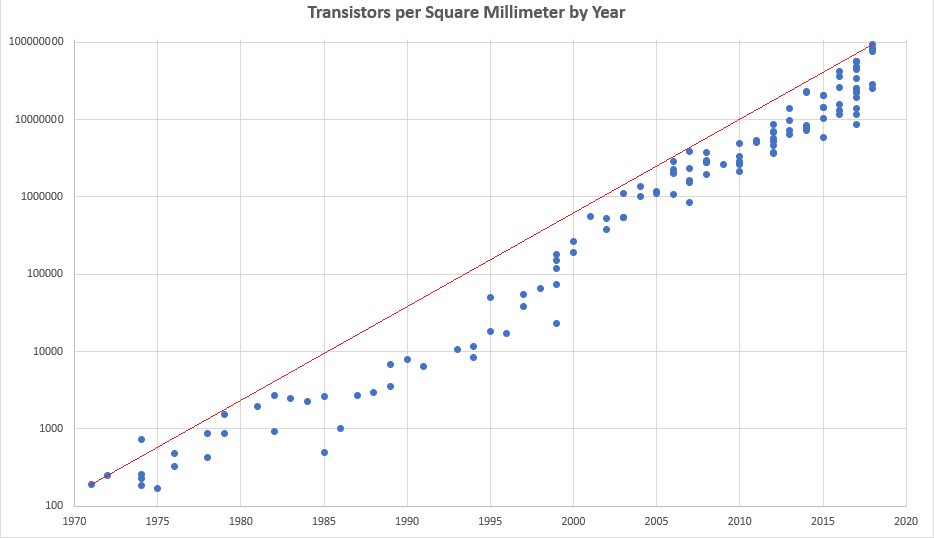
\includegraphics[width=0.76\linewidth]{Moores_Law}
		\caption[Legge di Moore]{Rappresentazione della legge di Moore: l'aumento del numero di transistor in un chip su scala logaritmica rispetto al passare degli anni. Fonte: \url{https://medium.com/predict/moores-law-is-alive-and-well-eaa49a450188}}
		\label{fig:mooreslaw}
	\end{figure}
	
	Intorno al 2007, sono apparse sul mercato le prime General-Purpose Graphic Processing Unit (GPGPU), ovvero le prime schede grafiche programmabili in maniera generica. Ciò non significa che, prima di quella data, non fossero programmabili ma si intende dire che erano utilizzabili solamente per applicazioni strettamente legate alla grafica. Le GPGPU hanno aperto una nuova era del calcolo parallelo, permettendo ai programmatori di sfruttare l'elevatissimo numero di core fisici per computazioni estremamente parallelizzabili. La differenza principale, a livello hardware, tra una CPU multi-core e una GPGPU consiste infatti nel numero di core molto maggiore nella seconda, come mostra la figura \ref{fig:cpu-gpu-computing-architecture}. Questa abbondanza di risorse di calcolo ha cambiato anche il modo di strutturare e progettare i programmi paralleli.
	
	\begin{figure}[!ht]
		\centering
		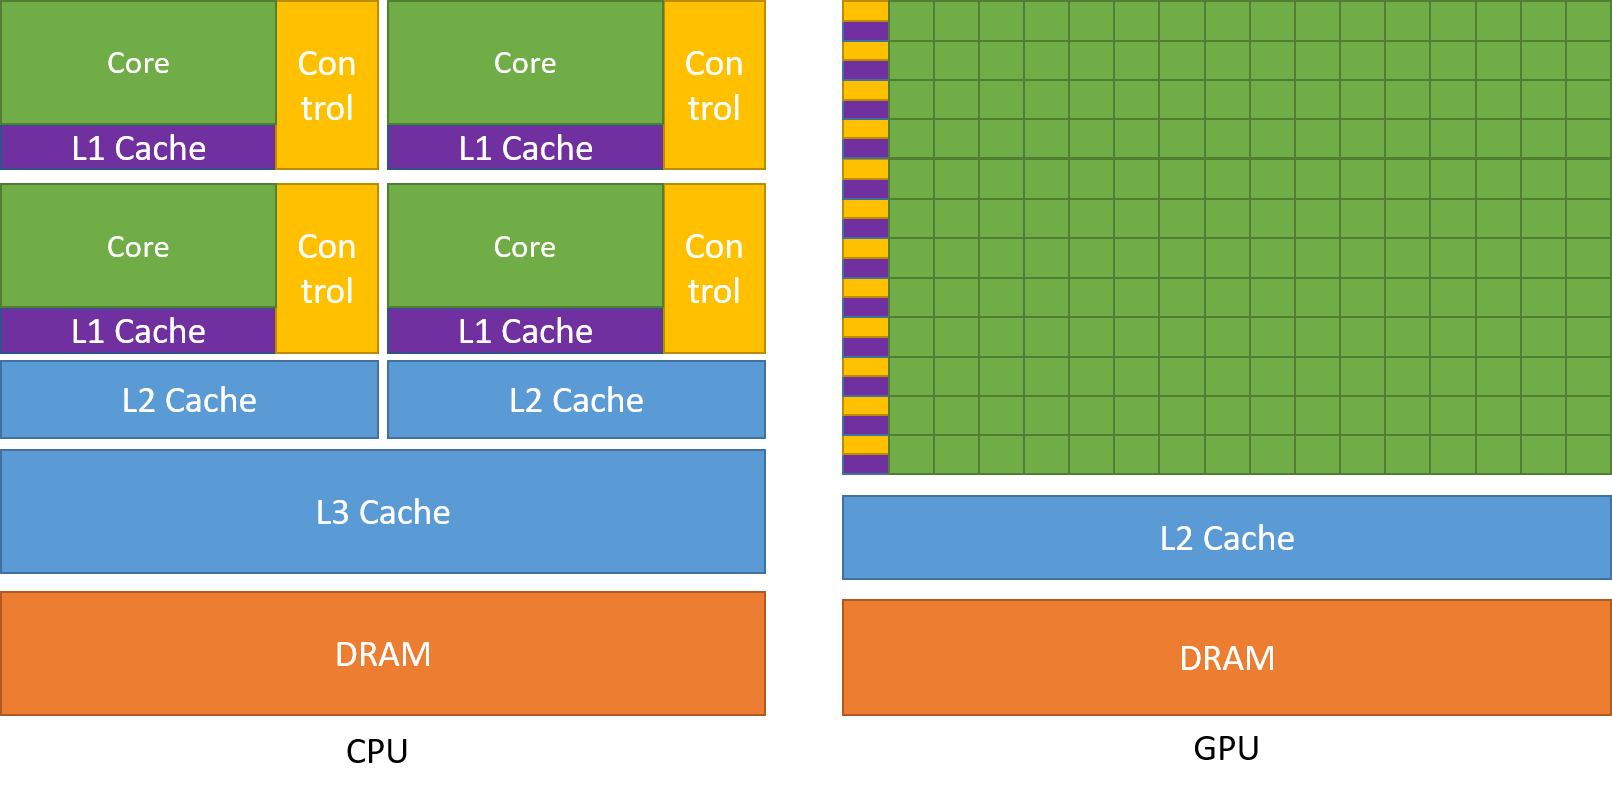
\includegraphics[width=\linewidth]{cpu-gpu-computing-architecture}
		\caption[Differenza architetturale tra CPU e GPU]{A sinistra l'architettura di una classica CPU, a destra l'architettura di una GPGPU. Fonte: \url{https://docs.nvidia.com/cuda/cuda-c-programming-guide/index.html}}
		\label{fig:cpu-gpu-computing-architecture}
	\end{figure}
	
	\section{GPU e CUDA}
	CUDA (acronimo di Compute Unified Device Architecture) è un'architettura hardware realizzata da NVIDIA, la cui prima versione è stata pubblicata nel 2007. Tramite CUDA è possibile scrivere programmi che eseguono parte del loro codice su una scheda grafica NVIDIA. CUDA basa tutto il suo funzionamento su alcuni concetti molto semplici: la CPU su cui viene lanciato il programma è chiamata \textit{host} e può interagire con una o più schede grafiche NVIDIA, chiamate \textit{device}. L'host può invocare alcune funzioni specifiche che vengono eseguite dal device. L'esecuzione di queste funzioni è asincrona, ovvero il controllo viene restituito subito all'host, senza attendere il termine dell'esecuzione. Tuttavia, esiste la possibilità di sincronizzare esplicitamente l'host con un device. Le funzioni più importanti sono i \textit{kernel}, le uniche che possono essere scritte dal programmatore, che possono effettuare qualunque tipo di calcolo. Anche i kernel sono eseguiti in maniera asincrona ma, a differenza delle altre funzioni, richiedono due parametri obbligatori, ovvero il numero di blocchi e il numero di thread per ogni blocco da utilizzare per l'esecuzione.
	
	CUDA raggruppa logicamente tutti i thread, ovvero le singole unità di esecuzione logiche, in blocchi che a loro volta sono raggruppati in una griglia. Ogni device ha sempre e solo una griglia in esecuzione e ogni griglia esegue sempre e solo un singolo kernel. \'E possibile identificare i blocchi e i thread mediante un indice a 1, 2 o 3 dimensioni in base all'occorrenza. Nella figura \ref{fig:grid-of-thread-blocks} è mostrato l'esempio di indicizzazione per una griglia bidimensionale formata da blocchi bidimensionali di thread.
	
	\begin{figure}[!ht]
		\centering
		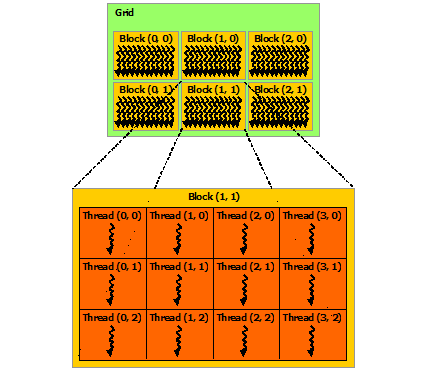
\includegraphics[width=0.5\textwidth]{grid-of-thread-blocks}
		\caption[Struttura della griglia di una GPU CUDA]{Suddivisione della griglia di una GPU CUDA in blocchi di thread. Fonte: \url{https://docs.nvidia.com/cuda/cuda-c-programming-guide/index.html}}
		\label{fig:grid-of-thread-blocks}
	\end{figure}
	
	La memoria di un device CUDA, come si nota dalla figura \ref{fig:cuda-memory-model}, è suddivisa in vari livelli:
	\begin{itemize}
		\item la \textbf{memoria globale} è la più voluminosa all'interno di un device (alcuni GB) ed è accessibile da tutti i thread di tutti i blocchi
		\item la \textbf{memoria texture} è molto più piccola di quella globale (alcuni MB) ed è ottimizzata per contenere dati di texture, è accessibile da tutti i thread di tutti i blocchi
		\item la \textbf{memoria delle costanti} è molto piccola (in genere 64KB) ed ottimizzata per il broadcast, è accessibile da tutti i thread di tutti i blocchi
		\item la \textbf{memoria condivisa} è più piccola (alcuni MB) ma molto più veloce di quella globale però è accessibile solamente da thread all'interno dello stesso blocco
		\item la \textbf{memoria locale} è quella "privata" di ogni thread e per questo motivo è accessibile solamente da esso
	\end{itemize}
	
	\begin{figure}[!ht]
		\centering
		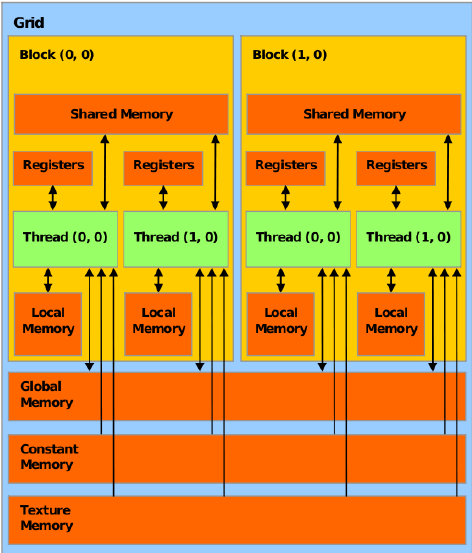
\includegraphics[width=0.5\textwidth]{CUDA-memory-model}
		\caption[Struttura della memoria di una GPU CUDA]{Struttura e gerarchia delle varie memorie all'interno di una GPU CUDA. Fonte: \url{https://www.researchgate.net/figure/CUDA-memory-model-from-7\_fig1\_4373162}}
		\label{fig:cuda-memory-model}
	\end{figure}

	\begin{wrapfigure}{r}{0.5\textwidth}
		\centering
		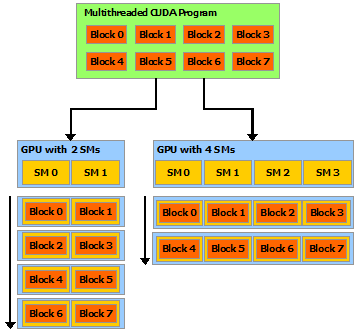
\includegraphics[width=0.45\textwidth]{automatic-scalability}
		\caption{Schedulazione automatica dei thread in una GPU CUDA.\\Fonte: \url{https://docs.nvidia.com/cuda/cuda-c-programming-guide/index.html}}
		\label{fig:automatic-scalability}
	\end{wrapfigure}
	
	Lo scheduling dei thread in una scheda CUDA funziona in modo particolare. Innanzitutto, va precisato che, nonostante il numero di core fisici (che in una scheda NVIDIA vengono chiamati Streaming Multiprocessors) vari tra una scheda e l'altra, non è possibile scegliere quali e quanti utilizzare per l'esecuzione di un kernel. Quando viene invocato un kernel, infatti, i thread richiesti vengono creati in memoria ma poi è l'hardware che sceglie automaticamente a \textit{runtime} la schedulazione migliore di questi thread sui SM a disposizione. La figura \ref{fig:automatic-scalability} mostra l'esempio di uno stesso programma eseguito su due schede con numero diverso di SM.

	Per questo motivo, si utilizza il concetto di \textit{thread warp}: un gruppo di thread (genericamente massimo 32) appartenenti allo stesso blocco che devono eseguire la stessa porzione di codice vengono schedulati tutti insieme sullo stesso SM ed eseguiti contemporaneamente. In caso di una biforcazione del flusso di controllo (ad esempio a causa di un costrutto \texttt{if-else} nel codice), viene calcolata la condizione per tutti i thread, dopodiché vengono eseguiti tutti insieme solamente quelli che hanno verificato la condizione (ovvero il ramo \texttt{if}), poi vengono eseguiti tutti insieme tutti gli altri (il ramo \texttt{else}). Nella figura \ref{fig:thread-warp} è mostrato l'esempio di una porzione di codice in cui i primi 16 thread eseguono il blocco di codice A mentre gli altri eseguono il blocco B.
	
	\begin{figure}[!ht]
		\centering
		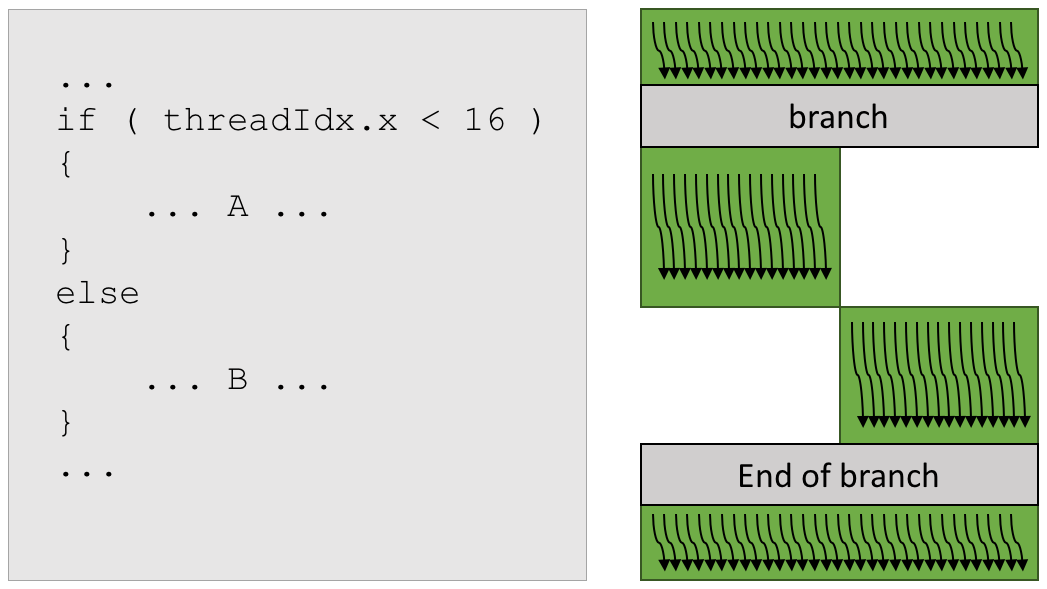
\includegraphics[width=0.7\linewidth]{thread-warp}
		\caption{Esecuzione di un thread warp in caso di biforcazione.\\Fonte: \url{https://subscription.packtpub.com/book/programming/9781788996242/3/ch03lvl1sec23/minimizing-the-cuda-warp-divergence-effect}}
		\label{fig:thread-warp}
	\end{figure}

	\begin{wrapfigure}{r}{0.5\textwidth}
		\centering
		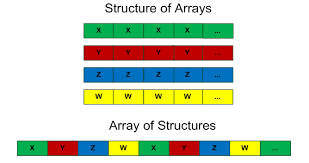
\includegraphics[width=0.5\textwidth]{aos-vs-soa}
		\caption{Differenza tra AoS e SoA. Fonte: \url{https://arxiv.org/ftp/arxiv/papers/1907/1907.05560.pdf}}
		\label{fig:aos-vs-soa}
	\end{wrapfigure}

	Va posta particolare attenzione anche al modo con cui i thread di una GPU CUDA accedono alla memoria. Infatti, la caratteristica più importante è il raggruppamento delle letture in memoria: se un certo numero di thread, appartenenti allo stesso warp, deve accedere in locazioni di memoria adiacenti, viene effettuata una singola operazione di lettura che trasferisce tutti i dati richiesti dai thread nelle rispettive memorie locali. Può sembrare una funzionalità irrilevante, ma in realtà può determinare differenze significative di prestazioni in programmi che non memorizzano i dati in maniera corretta. In particolare, esistono due pattern generali di memorizzazione: Array-of-Structures (AoS) e Structure-of-Arrays (SoA). Il primo, il più utilizzato, consiste nel memorizzare le caratteristiche di uno stesso elemento (come le coordinate di un punto) in locazioni adiacenti di memoria. Il secondo, invece, memorizza ogni dato in un array separato. Ipotizziamo che tutti i thread appartenenti ad un warp debbano leggere un valore dal vettore x (con riferimento alla figura \ref{fig:aos-vs-soa}) in posizioni adiacenti. Se i dati in questione fossero memorizzati come Structure-of-Arrays, tutti i valori richiesti si troverebbero all'interno dello stesso array adiacenti tra loro a partire da una certa posizione iniziale. La vicinanza in memoria di questi valori determina quindi un ridotto numero di letture effettive e un maggiore utilizzo del bus dati. Al contrario, se i dati fossero memorizzati tramite Array-of-Structures, i valori sarebbero più lontani fra loro e quindi richiederebbero un maggior numero di letture in memoria.
	
	\chapter{Teoria}
	\label{chap:teoria}
	\section{Grafi}
	Un grafo è una struttura matematica in cui un insieme di elementi, chiamati \textbf{nodi}, sono collegati tra loro mediante \textbf{archi}.	Un grafo è genericamente indicato come una coppia ordinata di insiemi $(V,E)$ in cui $V$ rappresenta l'insieme dei nodi ed $E$ l'insieme degli archi. Ogni elemento di $E$ consiste in una coppia ordinata di elementi di $V$, da cui segue che $E \subseteq V \times V$. Ad esempio, per il grafo \ref{fig:grafo-esempio} un nodo può essere $A$ e un arco può essere $(B,C)$. Una prima classificazione dei grafi consiste nel peso degli archi: un grafo si dice \textbf{non pesato} se i suoi archi hanno lo stesso peso (o, per semplicità, non hanno peso), altrimenti si definisce \textbf{pesato}. Un'ulteriore classificazione dei grafi consiste nell'orientamento degli archi: se almeno un arco ha una direzione si dice che il grafo è \textbf{orientato} (o diretto), altrimenti si dice \textbf{non orientato} (o indiretto).

	\begin{wrapfigure}{r}{0.5\textwidth}
		\centering
		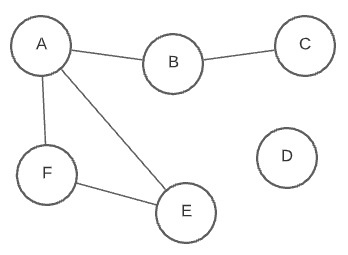
\includegraphics[width=0.5\textwidth]{grafo-esempio}
		\caption{Un esempio di grafo non orientato e non pesato}
		\source{https://it.wikipedia.org/\\wiki/Grafo}
		\label{fig:grafo-esempio}
	\end{wrapfigure}

	Se il grafo non è orientato, in genere si considera $E$ semplicemente come un insieme di coppie non ordinate di nodi in cui $(u,v)$ e $(v,u)$ rappresentano lo stesso arco.
	Inoltre, è possibile considerare anche i cosiddetti "cappi" o "auto-anelli", ovvero archi della forma $(u,u)$ che collegano un nodo con sè stesso. Se un grafo non possiede auto-anelli, allora si definisce \textbf{semplice}. In un grafo semplice il numero massimo possibile di archi è pari a $|V|\cdot (|V|-1)$, invece in un grafo non semplice corrisponde a $|V|^2$. Se il grafo è non orientato, il numero massimo di archi va diviso per 2. Se un grafo possiede esattamente il numero massimo di archi si dice \textbf{completo}.
	Una metrica molto utilizzata è la \textbf{densità} di un grafo, che si calcola come il rapporto tra il numero di archi e il numero massimo possibile di archi. Se un grafo ha "pochi" archi, dove per pochi si intende che il numero di archi è comparabile o inferiore al numero di nodi, si dice \textbf{sparso}, altrimenti \textbf{denso}. Gli archi diretti $(u,v)$ si dicono uscenti per il nodo $u$ ed entranti per il nodo $v$. Se un nodo non ha archi nè entranti nè uscenti, si dice \textbf{isolato} (nel grafo d'esempio, il nodo $D$ è isolato).
	
	Un grafo si dice planare se è possibile rappesentarlo su di un piano senza che nessuno dei suoi archi si intersechi con altri archi. Inoltre, un grafo planare è genericamente sparso a causa del limitato numero di archi che un nodo può avere.
	
	Un grafo può essere rappresentato in molti modi oltre a quello grafico. Il più conosciuto è la \textbf{matrice di adiacenza} che consiste in una matrice di dimensioni $|V|\times |V|$ in cui ogni elemento alla riga $i$ e alla colonna $j$ corrisponde al peso dell'arco diretto $(i,j)$. Computazionalmente parlando, richiede $O(|V|^2)$ spazio in memoria. Un altro metodo molto utilizzato è la \textbf{lista di adiacenza} in cui si memorizza una lista di nodi e ogni nodo memorizza la lista dei propri archi uscenti. Una lista di adiacenza richiede spazio $O(|V|+|E|)$. Infine, è possibile memorizzare un grafo come una lista di archi in cui ognuno contiene un riferimento ai nodi sorgente e destinazione e il proprio peso. Questo metodo richiede solamente $O(|E|)$ di memoria ma, essendo basato solamente sugli archi, non considera i nodi isolati.
	
	\section{Cammini minimi e problema SSSP}
	\label{section:sssp}
	In un grafo, un qualunque percorso che congiunge due nodi è detto \textbf{cammino} ed è rappresentabile come una lista ordinata di nodi. \'E importante notare la possibilità che uno stesso nodo sia presente più volte all'interno dello stesso cammino: quando ciò accade si parla di \textbf{cicli} (che approfondiremo di seguito). Il primo e l'ultimo nodo di questa lista ordinata sono chiamati rispettivamente \textbf{nodo sorgente} e \textbf{nodo destinazione}. In un grafo non pesato, il costo (o peso) di un cammino è pari al numero di nodi nella lista mentre in uno pesato è pari alla somma dei pesi degli archi coinvolti. Un cammino è detto \textbf{minimo} se non esiste un altro cammino nello stesso grafo, con uguali nodi sorgente e destinazione, con costo strettamente minore. Ad esempio, nel grafo della figura \ref{fig:grafo-esempio}, un cammino dal nodo B al nodo E può essere (B,A,F,E) mentre (B,A,E) è un cammino minimo. Va precisato che nello stesso grafo, a parità di nodi sorgente e destinazione, possono esistere numerosi cammini minimi diversi tra loro.
	
	Un ciclo consiste in un sottoinsieme di nodi di un grafo tali per cui è possibile raggiungere indirettamente, da qualunque nodo, uno qualunque degli altri nodi. Un albero, ad esempio, è un tipo particolare di grafo che non presenta cicli. Il costo (o peso) di un ciclo è pari alla somma dei pesi degli archi tra i nodi da cui è composto (nei grafi non pesati, invece, è pari al numero di nodi). Nel grafo della figura \ref{fig:grafo-esempio}, l'unico ciclo presente è (A,F,E). \'E possibile che in un grafo pesato siano presenti archi di costo negativo: sebbene siano poche le situazioni reali modellabili in questo modo, è molto importante determinare la presenza di cicli di costo negativo. Se in un grafo è presente un ciclo di costo negativo, allora ogni cammino minimo (in cui è possibile raggiungere tale ciclo dal nodo sorgente) avrà costo $-\infty$. Ai fini computazionali, non riuscire ad individuare un ciclo di costo negativo può determinare lo spreco di molte risorse di calcolo e di tempo eseguendo un algoritmo che produce un risultato inutile. Per questo motivo, in genere si utilizzano grafi con pesi strettamente positivi oppure algoritmi capaci di rilevare tali cicli.
	
	Un cammino minimo rispetta la cosiddetta \textbf{proprietà della sottostruttura ottima}, ovvero separando un cammino minimo in qualunque suo punto si ottengono due cammini minimi. Più formalmente, se abbiamo un cammino minimo $C$ dal nodo $u$ al nodo $v$ in cui è incluso anche il nodo $t$, allora sappiamo che tutti i nodi in $C$ da $u$ a $t$ costituiscono un cammino minimo e anche tutti i nodi in $C$ tra $t$ e $v$. Prendiamo come esempio il grafo della figura \ref{fig:grafo-esempio-2}. L'unico cammino minimo dal nodo A al nodo F è (A,D,F), di costo 8. \'E facile notare come il cammino (A,D) sia l'unico cammino minimo tra i nodi A e D e lo stesso vale per il cammino (D,F).
	
	\begin{wrapfigure}{r}{0.5\textwidth}
		\centering
		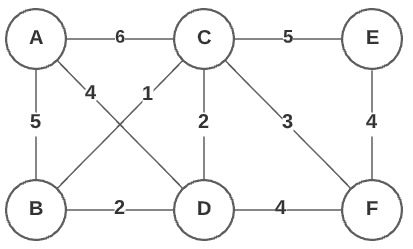
\includegraphics[width=0.5\textwidth]{grafo-esempio-2}
		\caption{Un esempio di grafo pesato non orientato}
		\source{http://www.mat.uniroma2.it/\\~guala/grafi\_2017.pdf}
		\label{fig:grafo-esempio-2}
	\end{wrapfigure}
	
	Dei tanti problemi che si possono applicare ad un grafo, il più studiato (su cui si concentra questa tesi) è senz'altro il Single-Source Shortest Path (abbreviato SSSP). Esso consiste, dato un grafo $G=(V,E)$ e un nodo sorgente $s$, nel trovare tutti i cammini minimi in $G$ che partono da $s$ e terminano in ogni altro nodo. Letteralmente significa "cammino minimo a singola sorgente", per differenziarlo dalla sua versione generalizzata, l'All-Pairs Shortest Path (APSP) che invece chiede di trovare il cammino minimo per ogni coppia di vertici. Il risultato del SSSP consiste in un array di distanze dal nodo sorgente e in un array di predecessori tramite cui è possibile costruire l'albero dei cammini minimi.
	
	\chapter{L'algoritmo di Bellman-Ford}
	\label{chap:analisi}
	\section{Analisi dello pseudocodice}
	Proposto per primo dal matematico Alfonso Shimbel nel 1955 \cite{Shimbel1955}, questo algoritmo è chiamato Bellman-Ford perché Richard Bellman, nel 1958 \cite{Bellman1958}, e Lester Ford Jr., nel 1956 \cite{Ford1956}, hanno pubblicato un articolo in cui presentavano lo stesso algoritmo. Ford lo propose come soluzione al problema logistico di trasportare un certo numero di beni da un punto A ad un punto B. Invece, Bellman lo propose come soluzione al problema più realistico di trovare il percorso più veloce attraverso una rete di città collegate tra loro. Edward F. Moore ha poi pubblicato una sua variante nel 1959 \cite{Moore1959} (per questo a volte viene chiamato Bellman-Ford-Moore) che riduce drasticamente il numero di rilassamenti da effettuare ad ogni iterazione. La variante di Moore è nota come Shortest Path Faster Algorithm. Yen nel 1970 \cite{Yen1970} ha pubblicato una complicata ottimizzazione che riduce il numero totale di iterazioni da $|V|-1$ a $|V|/2$. Bannister e Eppstein, infine, nel 2012 \cite{Bannister2012} hanno migliorato la variante di Yen riducendo il numero di iterazioni a $|V|/3$.
	
	La versione che riportiamo di seguito e che andremo ad implementare è quella originale proposta prima da Lester Ford Jr. e poi da Richard Bellman.
	
	\begin{algorithm}
		\SetAlgorithmName{Bellman-Ford}{}{}
		\KwIn{G, w, s}
		\KwResult{FALSE se il grafo G contiene cicli di costo negativo, TRUE altrimenti}
		Initialize-Single-Source(G,s)\;
		\For{i=1 \textbf{to} |G.V| - 1}{
			\ForEach{edge (u,v) $\in$ G.E}{
				Relax(u,v,w)\;
			}
		}
		\ForEach{edge (u,v) $\in$ G.E}{
			\If{v.d > u.d + w(u,v)}{
				\Return FALSE\;
			}
		}
		\Return TRUE\;
		\caption{L'algoritmo di Bellman-Ford}
		\label{alg:bf}
	\end{algorithm}

	Come è possibile notare dallo pseudocodice, il corpo effettivo dell'algoritmo consiste nelle righe 2-6. Difatti, \texttt{Initialize-Single-Source} (algoritmo \ref{alg:init}) è una procedura molto semplice che imposta la distanza di ogni nodo dalla sorgente a $+\infty$ e poi azzera la distanza del nodo sorgente. Il codice nelle righe 7-11 consiste invece in un ciclo per verificare o meno la presenza di cicli di costo negativo.
	
	\begin{algorithm}
		\SetAlgorithmName{Initialize-Single-Source}{}{}
		\KwIn{G, s}
		\ForEach{vertex v $\in$ G.V}{
			v.d = $\infty$\;
			v.$\pi$ = NIL\;
		}
		s.d = 0\;
		\caption{La procedura di inizializzazione del grafo}
		\label{alg:init}
	\end{algorithm}
	
	Il corpo dell'algoritmo esegue un'operazione di rilassamento (o meglio, invoca la procedura Relax) su ogni arco del grafo per $|V|-1$ iterazioni. Questo limite nasce dal numero di rilassamenti effettuati nel caso pessimo. Consideriamo, ad esempio, un grafo in cui tutti i nodi sono collegati in linea, ognuno è collegato solo con il precedente ed il successivo tranne il primo e l'ultimo che hanno un solo arco. Se la sorgente è il primo nodo, l'algoritmo di Bellman-Ford dovrà effettuare esattamente $|V|-1$ iterazioni di rilassamento perché coincide con il numero di archi nel cammino più lungo all'interno del grafo e ogni iterazione di rilassamento rilassa almeno un arco. Come si può notare, questo algoritmo effettua un'enorme quantità di calcoli inutili ed è proprio per questo che sono state proposte molte ottimizzazioni per ridurre il più possibile sia il numero complessivo di iterazioni di rilassamento che il numero di rilassamenti in ogni iterazione. Ad esempio, il limite massimo di iterazioni di rilassamento da effettuare corrisponde alla lunghezza del cammino minimo più lungo del grafo (molto inferiore al numero di nodi nel caso di grafi densi). Un'ulteriore ottimizzazione può essere il controllo sugli effettivi rilassamenti effettuati durante un'iterazione: se non sono stati effettuati rilassamenti nell'iterazione corrente, sicuramente non ne verranno effettuati altri in quelle successive e quindi l'algoritmo può terminare. Infine, è inefficiente effettuare un rilassamento su ogni arco del grafo al di fuori della prima iterazione. In tutte le successive iterazioni, è sufficiente effettuare un rilassamento solamente sugli archi adiacenti ad almeno un arco che è stato rilassato nell'iterazione precedente.
	
	La procedura Relax (algoritmo \ref{alg:relax}) richiede in input due nodi ($u$ e $v$) e la funzione $w$ che restituisce, dati due nodi, il peso dell'arco tra i due. Questa procedura non consiste in un effettivo rilassamento dell'arco $(u,v)$ ma è un tentativo di rilassamento, infatti viene verificato se una riduzione della distanza del nodo $v$ dalla sorgente sia possibile. In parole povere, la procedura Relax verifica se "arrivare al nodo $v$ passando per $u$ come ultimo nodo" sia meno costoso del valore già presente.
	
	\begin{algorithm}
		\SetAlgorithmName{Relax}{}{}
		\KwIn{u, v, w}
		\If{v.d > u.d + w(u,v)}{
			v.d = u.d + w(u,v)\;
			v.$\pi$ = u\;
		}
		\caption{La procedura di rilassamento di un arco}
		\label{alg:relax}
	\end{algorithm}
	
	L'algoritmo di Bellman-Ford riesce a rilevare i cicli di costo negativo verificando se è possibile rilassare un arco alla fine delle $|V|-1$ iterazioni. Se in un grafo è presente un ciclo di costo negativo, almeno un arco di quel ciclo verrà rilassato ad ogni iterazione. Questo è dovuto alla presenza di almeno un arco di costo negativo che permette sempre di ridurre la distanza dal nodo sorgente. Come già spiegato nella sezione \ref{section:sssp}, quando è presente un ciclo di costo negativo è sempre possibile ridurre il costo di un cammino che passa per esso. Per questo motivo, se alla fine delle $|V|-1$ iterazioni, almeno un arco è ancora rilassabile, allora vuol dire che è presente un ciclo di costo negativo e l'arco rilassabile ne fa parte.

	\section{Costo computazionale}
	La procedura \texttt{Initialize-Single-Source} esegue due operazioni di costo $O(1)$ in ciascuna delle $|V|$ iterazioni e infine una singola istruzione di costo $O(1)$. Dunque, il suo costo computazionale complessivo è $O(|V|)$. La procedura Relax esegue un confronto e, se verificato, esegue due istruzioni di costo $O(1)$. Complessivamente, dunque, la procedura Relax ha costo computazionale $O(1)$. Le istruzioni tra le righe 2-6 dell'algoritmo sono un doppio ciclo annidato che, per ognuna delle $|V|-1$ iterazioni, invoca la procedura Relax su ogni arco, dunque per $|E|$ volte. Quindi, questa porzione dell'algoritmo ha un costo computazionale di $O(|V|\cdot |E|)$. Le istruzioni sulle righe 7-11 complessivamente hanno un costo di $O(|E|)$ poichè esegue un confronto (di costo costante) per $|E|$ volte. Complessivamente, l'algoritmo ha costo computazionale $O(|V|\cdot |E|)$.
	
	\section{Dove parallelizzare}
	Analizziamo ora le dipendenze tra dati contenuti nell'algoritmo. Ognuna delle iterazioni del ciclo sulle righe 2-6 è dipendente dal risultato dell'iterazione precedente. Mentre ogni iterazione del ciclo tra le righe 3-5 presenta una dipendenza particolare: ogni rilassamento di un arco $(u,v)$ dipende dal risultato dell'ultimo rilassamento di un arco diretto verso $v$.
	
	Alternativamente, questo algoritmo può essere alterato scambiando l'ordine dei due cicli annidati. Questa variazione lo rende incorretto solamente se seriale. Se consideriamo una versione parallela di questa variante, si può interpretare il lavoro effettuato da un singolo thread come un rilassamento seguito da massimo $|V|-1$ tentativi di aggiornamento concorrente del valore della distanza di $v$.
	
	\section{Precisazioni}
	Siccome, per lo scopo di questa tesi, non è necessario che l'algoritmo riesca a costruire l'albero dei cammini minimi, non è stata implementata questa funzionalità. Con riferimento allo pseudocodice, questa modifica si traduce nella rimozione della riga 3 dalle procedure Relax (algoritmo \ref{alg:relax}) e di inizializzazione (algoritmo \ref{alg:init}). Inoltre, i test utilizzati per le misurazioni non presentano archi di costo negativo e di conseguenza nessun ciclo di costo negativo. Per questo motivo, l'algoritmo implementato produce solamente un array di distanze di ogni nodo dalla sorgente.
	
	\chapter{Progettazione}
	\label{chap:progettazione}
	Basandoci sull'analisi effettuata nel capitolo precedente, proponiamo di seguito tre implementazioni differenti dell'algoritmo di Bellman-Ford.
	
	\section{La versione \texttt{bf0}}
	La prima versione sfrutta pesantemente il parallelismo massivo offerto da CUDA, memorizzando il grafo di input come un array di archi e parallelizzando il ciclo "interno" dell'algoritmo utilizzando un thread per ogni arco del grafo. Ad ogni iterazione, ogni thread esegue una procedura Relax su un singolo arco del grafo e poi si sincronizza con tutti gli altri.
	
	Il problema principale di questa versione consiste negli aggiornamenti concorrenti della distanza del nodo $v$. Come già accennato in precedenza, possiamo interpretare il lavoro svolto da ogni thread come $|V|-1$ tentativi di aggiornamento di un singolo valore. Per questo motivo, riteniamo possa essere comunque corretta una versione che non utilizza meccanismi di mutua esclusione. Tale versione sarà chiamata \texttt{bf0-none}. Ovviamente proponiamo anche la sua controparte \texttt{bf0-mutex} perchè garantisce la correttezza del risultato al prezzo dell'impiego di operazioni atomiche.
	
	\begin{table}[!ht]
		\centering
		\begin{tabular}{|l|c|c|c|}
			\hline
			\textbf{Nome versione} & \textbf{Mutex} & \textbf{AoS/SoA} & \textbf{Shared Memory} \\ \hline
			\texttt{bf0-none-aos-nosh}  & no & AoS & no \\ \hline
			\texttt{bf0-none-aos-sh}    & no & AoS & si \\ \hline
			\texttt{bf0-none-soa-nosh}  & no & SoA & no \\ \hline
			\texttt{bf0-none-soa-sh}    & no & SoA & si \\ \hline
			\texttt{bf0-mutex-aos-nosh} & si & AoS & no \\ \hline
			\texttt{bf0-mutex-aos-sh}   & si & AoS & si \\ \hline
			\texttt{bf0-mutex-soa-nosh} & si & SoA & no \\ \hline
			\texttt{bf0-mutex-soa-sh}   & si & SoA & si \\ \hline
		\end{tabular}
		\label{tab:riassunto_bf0}
		\caption{Tabella riassuntiva delle caratteristiche delle versioni dell'algoritmo \texttt{bf0}}
	\end{table}
	
	\section{Rimuovere i mutex: \texttt{bf1}}
	\label{section:intro-bf1}
	Il problema degli aggiornamenti concorrenti può essere risolto senza mutex ma utilizzando un numero molto inferiore di thread. Se il grafo di input viene memorizzato come lista di adiacenza in cui ogni nodo ha un riferimento solo ai nodi raggiungibili tramite archi uscenti, allora noi possiamo parallelizzare i rilassamenti da effettuare su ogni nodo. Nel dettaglio, fissato un nodo $u$, utilizziamo un thread per ogni arco uscente da $u$ che vi effettua un rilassamento. Com'è evidente, questa versione non presenta il problema di aggiornamenti concorrenti, ma utilizza molti meno thread. Probabilmente, le prestazioni di questa versione potrebbero essere comparabili a quella precedente solamente su grafi piccoli e completi, in cui ogni nodo ha un elevato numero di archi uscenti.
	
	\begin{table}[!ht]
		\centering
		\begin{tabular}{|l|c|c|}
			\hline
			\textbf{Nome versione} & \textbf{AoS/SoA} & \textbf{Shared Memory} \\ \hline
			\texttt{bf1-aos-nosh}  & AoS & no \\ \hline
			\texttt{bf1-aos-sh}    & AoS & si \\ \hline
			\texttt{bf1-soa-nosh}  & SoA & no \\ \hline
			\texttt{bf1-soa-sh}    & SoA & si \\ \hline
		\end{tabular}
		\label{tab:riassunto_bf1}
		\caption{Tabella riassuntiva delle caratteristiche delle versioni dell'algoritmo \texttt{bf1}}
	\end{table}
	
	\section{Sfruttare più thread: \texttt{bf2}}
	Il difetto maggiore della versione \texttt{bf1} è il suo ridottissimo numero di thread. \'E possibile, però, sfruttare un numero maggiore di thread al prezzo di introdurre nuovamente degli aggiornamenti concorrenti. In questo caso il grafo dovrebbe essere memorizzato come una lista di adiacenza in cui ogni nodo memorizza il riferimento ai nodi che possono raggiungerlo, dunque gli archi entranti. Con questa modifica, il numero di thread utilizzabili aumenta considerevolmente perché è possibile effettuare tutti i rilassamenti degli archi entranti su ogni nodo del grafo contemporaneamente. Per questi motivi, la versione \texttt{bf2} utilizzerà un blocco di thread per ogni nodo del grafo.

	\begin{table}[!ht]
		\centering
		\begin{tabular}{|l|c|c|}
			\hline
			\textbf{Nome versione} & \textbf{AoS/SoA} & \textbf{Shared Memory} \\ \hline
			\texttt{bf2-aos-nosh}  & AoS & no \\ \hline
			\texttt{bf2-aos-sh}    & AoS & si \\ \hline
			\texttt{bf2-soa-nosh}  & SoA & no \\ \hline
			\texttt{bf2-soa-sh}    & SoA & si \\ \hline
		\end{tabular}
		\label{tab:riassunto_bf2}
		\caption{Tabella riassuntiva delle caratteristiche delle versioni dell'algoritmo \texttt{bf2}}
	\end{table}
	
	\section{Dettagli implementativi}
	\label{section:impl}
	Di seguito si elencano alcuni dettagli o limiti non trascurabili presentati dalle versioni implementate.
	
	Come già spiegato nel capitolo \ref{chap:analisi}, ogni algoritmo che risolve il problema SSSP necessita dell'indice del nodo sorgente. In tutte le versioni implementate, il nodo sorgente è il nodo di indice $0$.
	
	Inoltre, in tutte le versioni implementate il peso di un arco è memorizzato come un numero intero. L'unica eccezione è costituita dalle versioni \texttt{bf0-mutex} in cui il peso di un arco è implementato mediante un \texttt{float} a 32 bit. Ciò è dovuto alla necessità di implementare il meccanismo di mutua esclusione: rispetto ad un'esplicita acquisizione e rilascio di una variabile mutex si è preferito utilizzare la funzione CUDA \texttt{atomicCAS}. L'utilizzo di un numero intero per il peso di un arco si è tradotto in un overflow durante il rilassamento, per questo motivo, in tutte le versioni (esclusa \texttt{bf0-mutex}) è stato implementato un controllo che non produce overflow che però non ha più la stessa struttura della procedura Relax (algoritmo \ref{alg:relax}). L'algoritmo \ref{alg:relax-no-overflow} rappresenta lo pseudocodice della procedura Relax effettivamente implementata.
	
	\begin{algorithm}
		\SetAlgorithmName{Relax-No-Overflow}{}{}
		\KwIn{u, v, w}
		\If{v.d > u.d \textbf{and} v.d - u.d > w(u,v)}{
			v.d = u.d + w(u,v)\;
		}
		\caption{La procedura di rilassamento di un arco che non produce overflow}
		\label{alg:relax-no-overflow}
	\end{algorithm}

	Tutti gli algoritmi che utilizzano un buffer all'interno della memoria condivisa (ovvero tutti i programmi con nome "\texttt{*-sh}"), lo utilizzano per ottimizzare gli accessi in lettura all'array dei dati di input (nel caso si usi AoS, altrimenti sui vari array di input per SoA). Nonostante l'array \texttt{distances} sia acceduto più volte, esso richiede anche un accesso in scrittura e tutti i suoi accessi in lettura non sono allineati. Questi fattori contribuiscono ad un peggioramento significativo delle prestazioni, anche in caso di utilizzo ibrido del buffer, misurato in maniera empirica i cui risultati non sono riportati in questa tesi.
	
	Tutte le versioni \texttt{bf0} utilizzano un thread per ogni arco del grafo e, considerato che nella maggior parte delle schede grafiche CUDA il numero massimo di thread per blocco è pari a 1024 e il numero massimo di blocchi utilizzabili è pari a $2^{31}$, il loro limite è pari a $2^{31}\cdot 1024$. Utilizzare come input un grafo con un numero maggiore di archi genererebbe un comportamento imprevisto.
	
	Le versioni \texttt{bf1} utilizzano un singolo blocco di $1024$ thread che opera su ogni nodo del grafo, ma non presenta limitazioni in questo senso.
	
	Le versioni \texttt{bf2}, siccome utilizzano un blocco di thread per ogni nodo, se utilizzate su grafi con un numero di nodi maggiore di $2^{31}$, possono generare un comportamento imprevisto.
	
	Le versioni \texttt{bf1}, siccome memorizzano il grafo come una lista di adiacenza basata sugli archi uscenti, se utilizzate su grafi in cui sono presenti nodi senza archi uscenti possono generare un comportamento imprevisto. Lo stesso problema è presente per le versioni \texttt{bf2} riguardo agli archi entranti. Le versioni \texttt{bf0}, invece, produrranno un valore di $+\infty$ per ogni nodo irraggiungibile.
	
	\chapter{Metriche di valutazione}
	\label{chap:metriche}
	\section{Speedup}
	Lo speedup è la principale metrica di misurazione di un programma parallelo. Essa, infatti, rappresenta l'accelerazione che un dato programma ha ricevuto tramite la parallelizzazione. In particolare, lo speedup di un programma parallelo eseguito con $p$ core si calcola come:
	\begin{equation}
		S(p) = \frac{T_s}{T(p)}
		\label{eq:speedup}
	\end{equation}
	in cui $T_s$ rappresenta il tempo di esecuzione del programma seriale (la "versione originale") e $T(p)$ rappresenta il tempo di esecuzione del programma parallelo utilizzando $p$ core.
	
	Idealmente, si vorrebbe ottenere uno \textbf{speedup lineare} nel proprio programma, ovvero $S(p) = p$ indipendentemente dal numero di processori utilizzati. Anche se può sembrare controintuitivo, raddoppiando il numero di processori impiegati non si ottiene quasi mai un dimezzamento perfetto del tempo di esecuzione; ciò è dovuto all'aumentare dei tempi per la sincronizzazione e la comunicazione, oltre all'\textit{overhead} per l'allocazione della memoria necessaria. Per questo motivo, lo speedup $S(p)$ è sempre inferiore a $p$. Nonostante ciò, esistono alcuni rari casi in cui è possibile misurare nella realtà uno \textbf{speedup superlineare}, ovvero $S(p) > p$. In questi casi, la misurazione indica che raddoppiando il numero di processori il tempo di esecuzione si è più che dimezzato. Questo fenomeno, più unico che raro, è dovuto nella maggior parte dei casi alle elevate velocità e dimensioni delle cache integrate all'interno dei processori utilizzati. Ad esempio, se i dati di un programma fossero abbastanza piccoli da poter risiedere interamente nella cache, il programma stesso otterrebbe una grande accelerazione per i tempi di accesso alla memoria.
	
	Come è possibile notare dalla formula \ref{eq:speedup}, lo speedup di un programma parallelo si osserva misurando il tempo di esecuzione man mano che si aumenta il numero di processori utilizzati. Questo non è possibile con un programma CUDA perché il programmatore non ha potere decisionale sul numero di core fisici da utilizzare nè sulla schedulazione dei thread logici: l'unico aspetto della computazione che può controllare è la dimensione della \textit{grid} (intesa come numero di blocchi e numero di thread per ciascun blocco). Per questo motivo, in genere non ha senso misurare lo speedup di un'applicazione parallela su CUDA semplicemente aumentando il numero di thread. Tuttavia, in questa tesi misuriamo un singolo valore di accelerazione per ogni algoritmo per meglio confrontare tra loro le varie versioni.
	
	\section{Throughput}
	Il throughput (o produttività) è una metrica molto più rappresentativa delle prestazioni di un'applicazione CUDA per i motivi citati nella sezione precedente. Esso consiste nel numero di "elementi" processati in un secondo, oppure di "unità di lavoro" eseguite nello stesso tempo. Cosa si intenda per unità di lavoro, però, dipende dal problema, dal tipo di dati in input e dall'implementazione di un certo algoritmo. Ad esempio, per un'applicazione che applica filtri di colore ad un'immagine il throughput può essere misurato come numero di pixel modificati al secondo. Un altro esempio può essere un'algoritmo che cerca la mossa migliore in una partita di scacchi per il quale la produttività si può misurare come il numero di stati della scacchiera analizzati ogni secondo. Nel nostro caso, il throughput è misurato come il numero di rilassamenti di un arco effettuati ogni secondo.
	
	Ogni algoritmo ha un limite massimo di throughput che è possibile raggiungere solamente aumentando le dimensioni dei dati di input. Per questo motivo, è molto importante misurare le prestazioni di un'applicazione impiegando test voluminosi.
	
	\chapter{Valutazione delle prestazioni}
	\label{chap:perf}
	\section{Descrizione dei test}
	I primi cinque test sono rappresentazioni sotto forma di grafo delle mappe stradali della città di Roma e di quattro paesi degli USA. Questi file sono reperibili ai link \cite{testUSA} e \cite{testRoma}. I successivi quattro test sono, invece, grafi sintetici casuali realizzati tramite il programma \texttt{graphgen} (disponibile nel repository \footnote{\url{https://github.com/Ledmington/bellman-ford-cuda}}) a densità crescente. L'impiego di questi ultimi si è rivelato necessario, al fine di una ricerca più completa possibile, dal momento che i primi quattro test non sono altro che grafi planari e, in quanto tali, hanno forti limitazioni sul numero di archi.
	
	Entrando più nello specifico, tutti i grafi elencati sono orientati, pesati e semplici. Solamente i primi 5 grafi sono planari. L'ultimo grafo, \texttt{100}, è l'unico completo. I primi cinque grafi sono considerati sparsi, gli ultimi quattro sono considerati densi. In nessuno di questi grafi sono presenti nodi isolati. La tabella \ref{tab:riassunto_test} contiene un breve riassunto delle caratteristiche di ogni test.
	\begin{table}[!ht]
		\centering
		\begin{tabular}{|c|c|c|c|}
			\hline
			\textbf{Nome test} & \textbf{Numero nodi} & \textbf{Numero archi} & \textbf{Descrizione} \\ \hline
			rome & 3353 & 8859 & Mappa metropolitana di Roma \\ \hline
			DE & 49109 & 119744 & Mappa stradale del Delaware \\ \hline
			VT & 97975 & 212979 & Mappa stradale del Vermont \\ \hline
			ME & 194505 & 425708 & Mappa stradale del Maine \\ \hline
			NV & 261155 & 618175 & Mappa stradale del Nevada \\ \hline
			025 & 1000 & 249808 & Grafo casuale con densità 0.25 \\ \hline
			050 & 1000 & 499574 & Grafo casuale con densità 0.5 \\ \hline
			075 & 1000 & 749262 & Grafo casuale con densità 0.75 \\ \hline
			100 & 1000 & 999000 & Grafo casuale completo \\ \hline
		\end{tabular}
		\caption{Tabella riassuntiva delle specifiche dei test utilizzati}
		\label{tab:riassunto_test}
	\end{table}
	
	\section{Specifiche hardware}
	Nella tabella \ref{tab:specs} sono riportate le specifiche hardware e software delle macchine utilizzate per la valutazione delle prestazioni degli algoritmi proposti. Le macchine saranno identificate tramite il nome della propria scheda grafica.
	
	\renewcommand{\arraystretch}{1.2}
	\begin{table}[!ht]
		\resizebox{\textwidth}{!}{
			\begin{tabular}{|l|c|c|c|}
				\hline
				& \textbf{940MX} & \textbf{GTX1070} & \textbf{RTX2080} \\ \hline
				\textbf{Sistema Operativo} & Windows & Ubuntu & Windows \\ \hline
				\textbf{Versione SO} & 10.0.19042.1165 & 16.04.7 & 10.0.19043.1165 \\ \hline
				\textbf{Compilatore C} & CL 19.29.30133 & GCC 5.4.0 & CL 19.29.30040 \\ \hline
				\textbf{Nome CPU} & Intel Core i5-7200U & Intel Xeon E5-2603 v4 & Intel Core i7-8700 \\ \hline
				\textbf{Frequenza CPU} & 2,5 - 2,7 GHz & 1,2 - 1,7 GHz & 3,2 GHz \\ \hline
				\textbf{Cores fisici} & 2 & 6 & 6 \\ \hline
				\textbf{Hyper-Threading} & si & no & si \\ \hline
				\textbf{L1 cache} & 128 KB & 32 KB & 384 KB \\ \hline
				\textbf{L2 cache} & 512 KB & 256 KB & 1,5 MB \\ \hline
				\textbf{L3 cache} & 3 MB & 15 MB & 12 MB \\ \hline
				\textbf{RAM totale} & 8 GB & 64 GB & 32 GB \\ \hline
				\textbf{Frequenza RAM} & 2133 MHz & 2400 MHz & 2133 MHz \\ \hline
				\textbf{Tipologia RAM} & DDR4 & DDR4 & DDR4 \\ \hline
				\textbf{Nome GPU} & GeForce 940MX & GeForce GTX1070 & GeForce RTX2080 \\ \hline
				\textbf{CUDA Driver} & 11.4 & 10.1 & 11.4 \\ \hline
				\textbf{CUDA Runtime} & 11.1 & 8.0 & 11.1 \\ \hline
				\textbf{CUDA capability} & 5.0 & 6.1 & 7.5 \\ \hline
				\textbf{Architettura GPU} & Maxwell & Pascal & Turing \\ \hline
				\textbf{Memoria globale} & 2 GB & 8 GB & 8 GB \\ \hline
				\textbf{Tipologia Memoria} & GDDR5 & GDDR5 & GDDR6 \\ \hline
				\textbf{Frequenza Memoria} & 2505 MHz & 4004 MHz & 7000 MHz \\ \hline
				\textbf{Ampiezza Bus} & 64 bit & 256 bit & 256 bit \\ \hline
				\textbf{Numero SM} & 3 & 15 & 46 \\ \hline
				\textbf{CUDA core totali} & 384 & 1920 & 2944 \\ \hline
				\textbf{Frequenza core} & 1189 MHz & 1797 MHz & 1860 MHz \\ \hline
			\end{tabular}
		}
		\caption{Specifiche hardware e software delle macchine utilizzate per le misurazioni}
		\label{tab:specs}
	\end{table}
	\renewcommand{\arraystretch}{1.1}

	\section{Prestazioni dell'algoritmo seriale}
	Nella tabella \ref{tab:performance_serial} sono riportati i valori di Wall Clock Time (tempo di esecuzione) e di throughput misurati sull'algoritmo \texttt{bf-serial} sulla CPU della macchina 940MX. Il tempo di esecuzione è espresso in secondi. Il throughput è espresso in milioni di operazioni di rilassamento effettuati al secondo ($10^6$ relax/s).
	
	\begin{table}[!ht]
		\centering
		\begin{tabular}{|c|c|c|}
			\hline
			\textbf{Nome test} & \textbf{Wall Clock Time} & \textbf{Throughput} \\ \hline
			       rome        &           0,38           &         78          \\ \hline
			        DE         &          81,45           &         75          \\ \hline
			        VT         &          217,06          &        95,8         \\ \hline
			        ME         &          874,61          &         94          \\ \hline
			        NV         &         1743,02          &         92          \\ \hline
			       025         &           2,39           &        104,2        \\ \hline
			       050         &           4,55           &        109,4        \\ \hline
			       075         &           6,8            &        109,8        \\ \hline
			       100         &           8,12           &        122,4        \\ \hline
		\end{tabular}
		\caption{Prestazioni dell'algoritmo seriale su CPU}
		\label{tab:performance_serial}
	\end{table}

	\section{Precisazioni preliminari}
	Tutti gli algoritmi producono il risultato corretto su ogni grafo utilizzato, tranne l'algoritmo \texttt{bf2-soa-sh} che produce valori errati per il grafo di Roma. Per questo motivo, tale algoritmo è considerato errato e non ne saranno riportate le misurazioni delle prestazioni.
	
	Inoltre, per gli algoritmi delle famiglie \texttt{bf1} e \texttt{bf2} non sono riportate le misurazioni per alcuni test come \texttt{NV}, \texttt{ME} e in alcuni casi \texttt{VT}. Non si è ritenuto utile riportarle in quanto i tempi di esecuzione, superiori ad un'ora, non sono comparabili con quelli raggiunti dagli algoritmi della famiglia \texttt{bf0}. Allo stesso modo, per gli stessi algoritmi e gli stessi test non sono riportati neanche i valori di throughput.
	
	\section{Speedup}
	Di seguito sono riportati i valori di speedup di ogni versione, misurati sui test a disposizione e su ogni scheda, rispetto al tempo d'esecuzione dell'algoritmo \texttt{bf-serial}.
	
	Innanzitutto, è possibile notare l'enorme differenza di speedup in generale tra la scheda 940MX e le altre. Evidente in particolar modo nelle figure \ref{fig:speedup_bf0-none} e \ref{fig:speedup_bf0-mutex}, ciò è dovuto soprattutto alla superiore potenza computazionale determinata dalle risorse hardware. Come già specificato nella tabella \ref{tab:specs}, non solo la frequenza di clock dei core CUDA è maggiore ma il numero stesso di core a disposizione è moltiplicato nelle schede GTX1070 e RTX2080.
	
	Nonostante i valori di speedup per gli algoritmi \texttt{bf0} siano molto simili tra di loro, si nota un modesto miglioramento da una qualunque versione \texttt{nosh} alla corrispettiva \texttt{sh}. I valori maggiori si ottengono su versioni che utilizzano AoS anche se sono molto più variabili rispetto ai valori misurati sugli algoritmi che utilizzano SoA.
	
	I valori misurati sul grafo \texttt{rome} sono estremamente ridotti (speedup compreso tra $1$ e $2$) a causa delle sue dimensioni.
	
	\begin{figure}[b]
		\centering
		\begin{subfigure}{.5\textwidth}
			\centering
			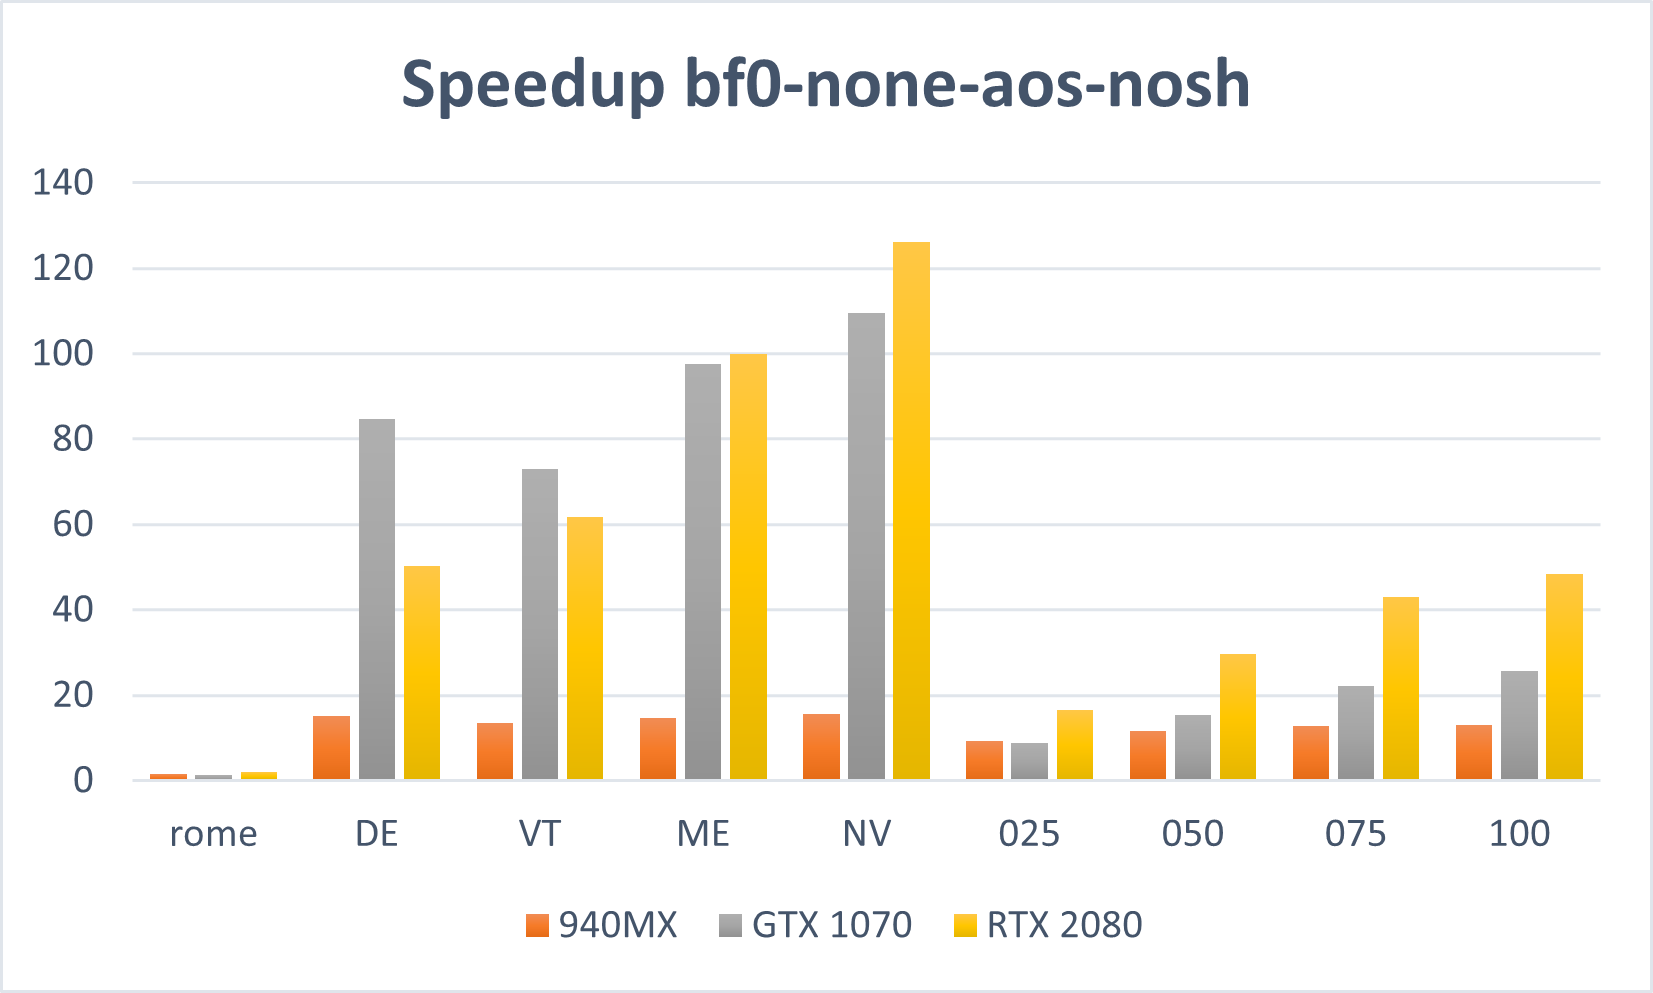
\includegraphics[width=\textwidth]{speedup_bf0-none-aos-nosh}
		\end{subfigure}%
		\begin{subfigure}{.5\textwidth}
			\centering
			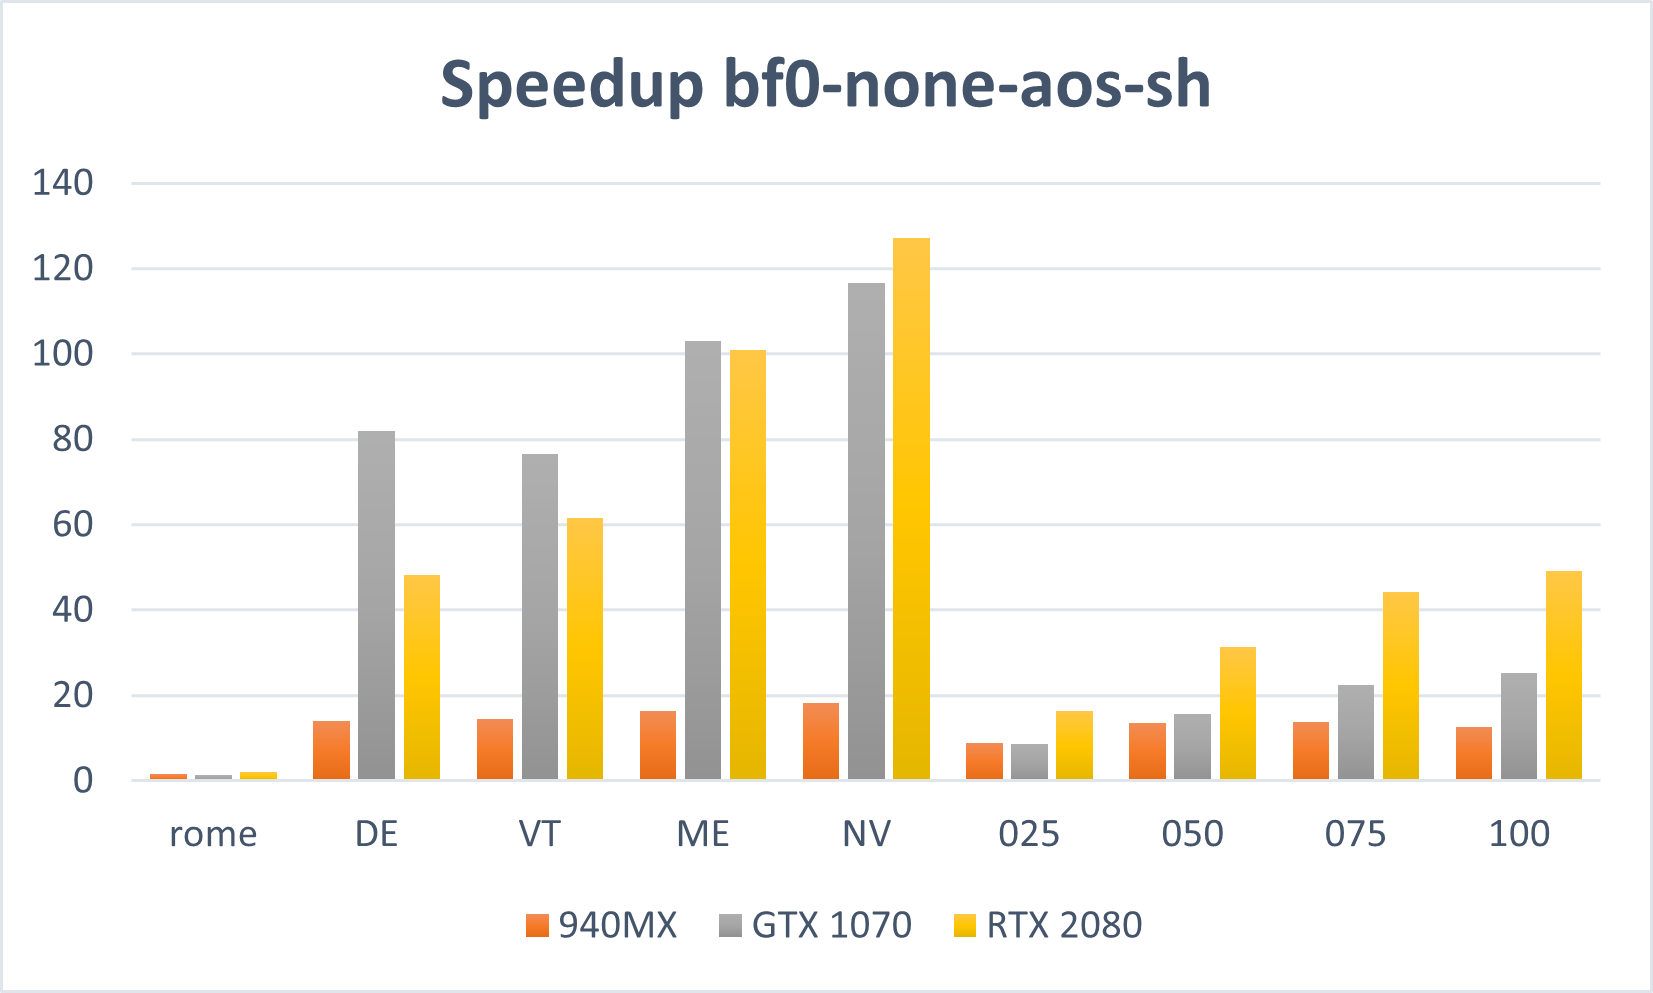
\includegraphics[width=\textwidth]{speedup_bf0-none-aos-sh}
		\end{subfigure}
		\begin{subfigure}{.5\textwidth}
			\centering
			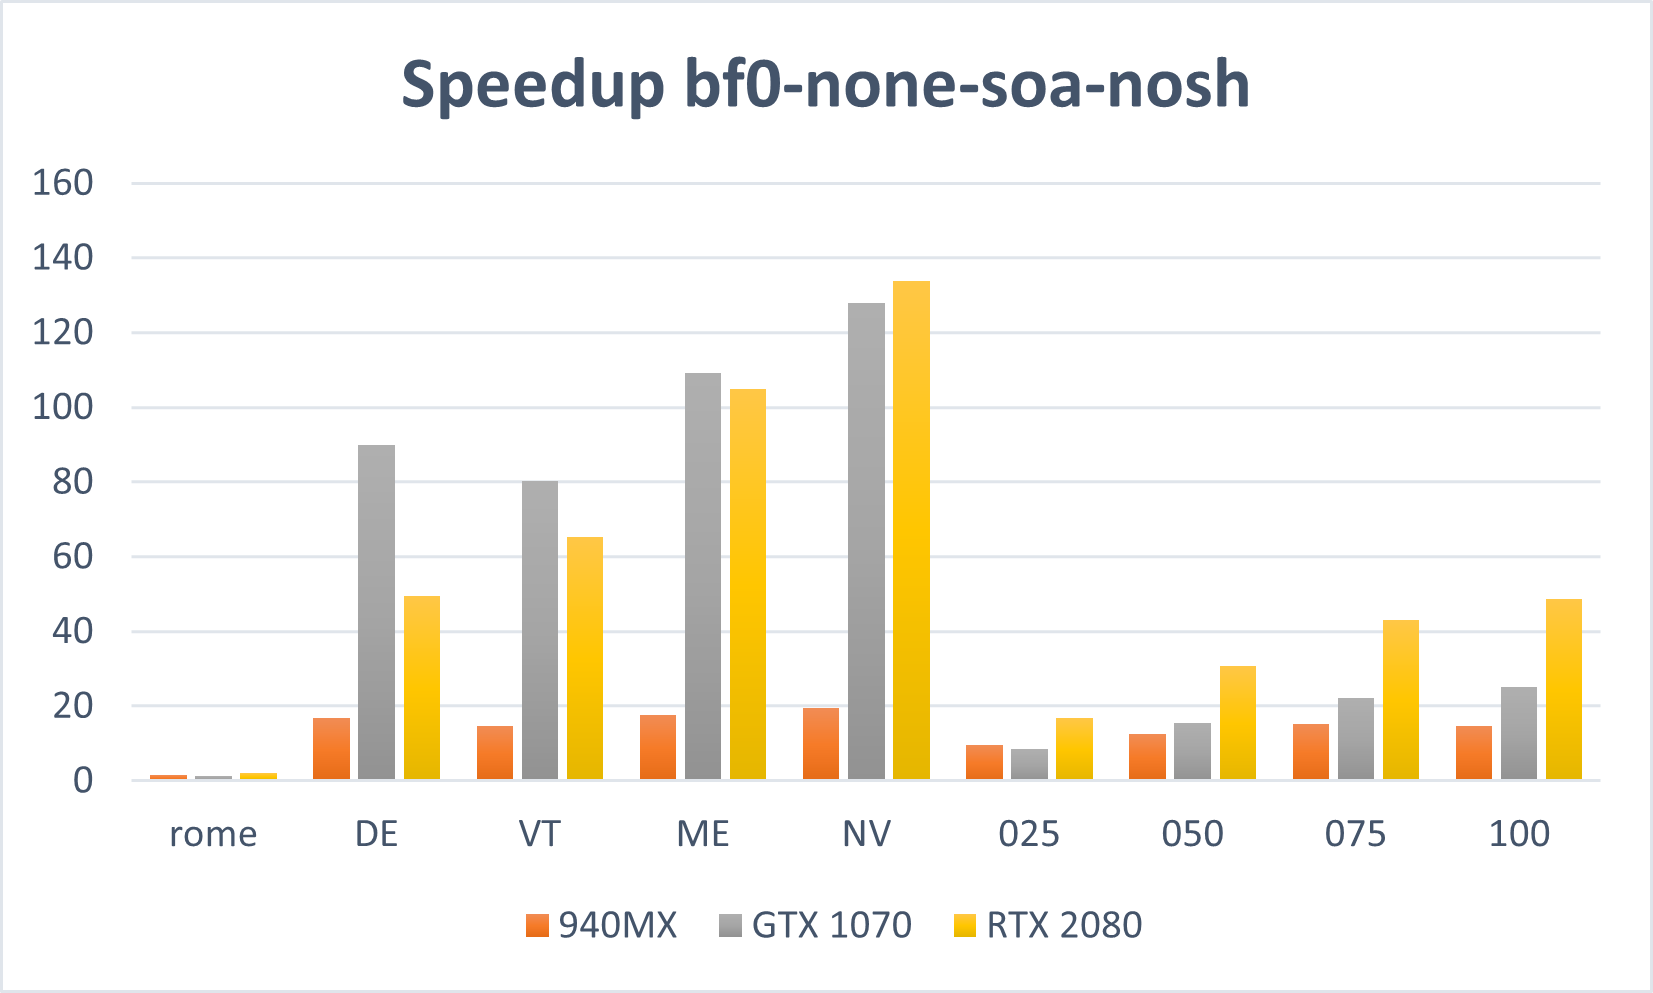
\includegraphics[width=\textwidth]{speedup_bf0-none-soa-nosh}
		\end{subfigure}%
		\begin{subfigure}{.5\textwidth}
			\centering
			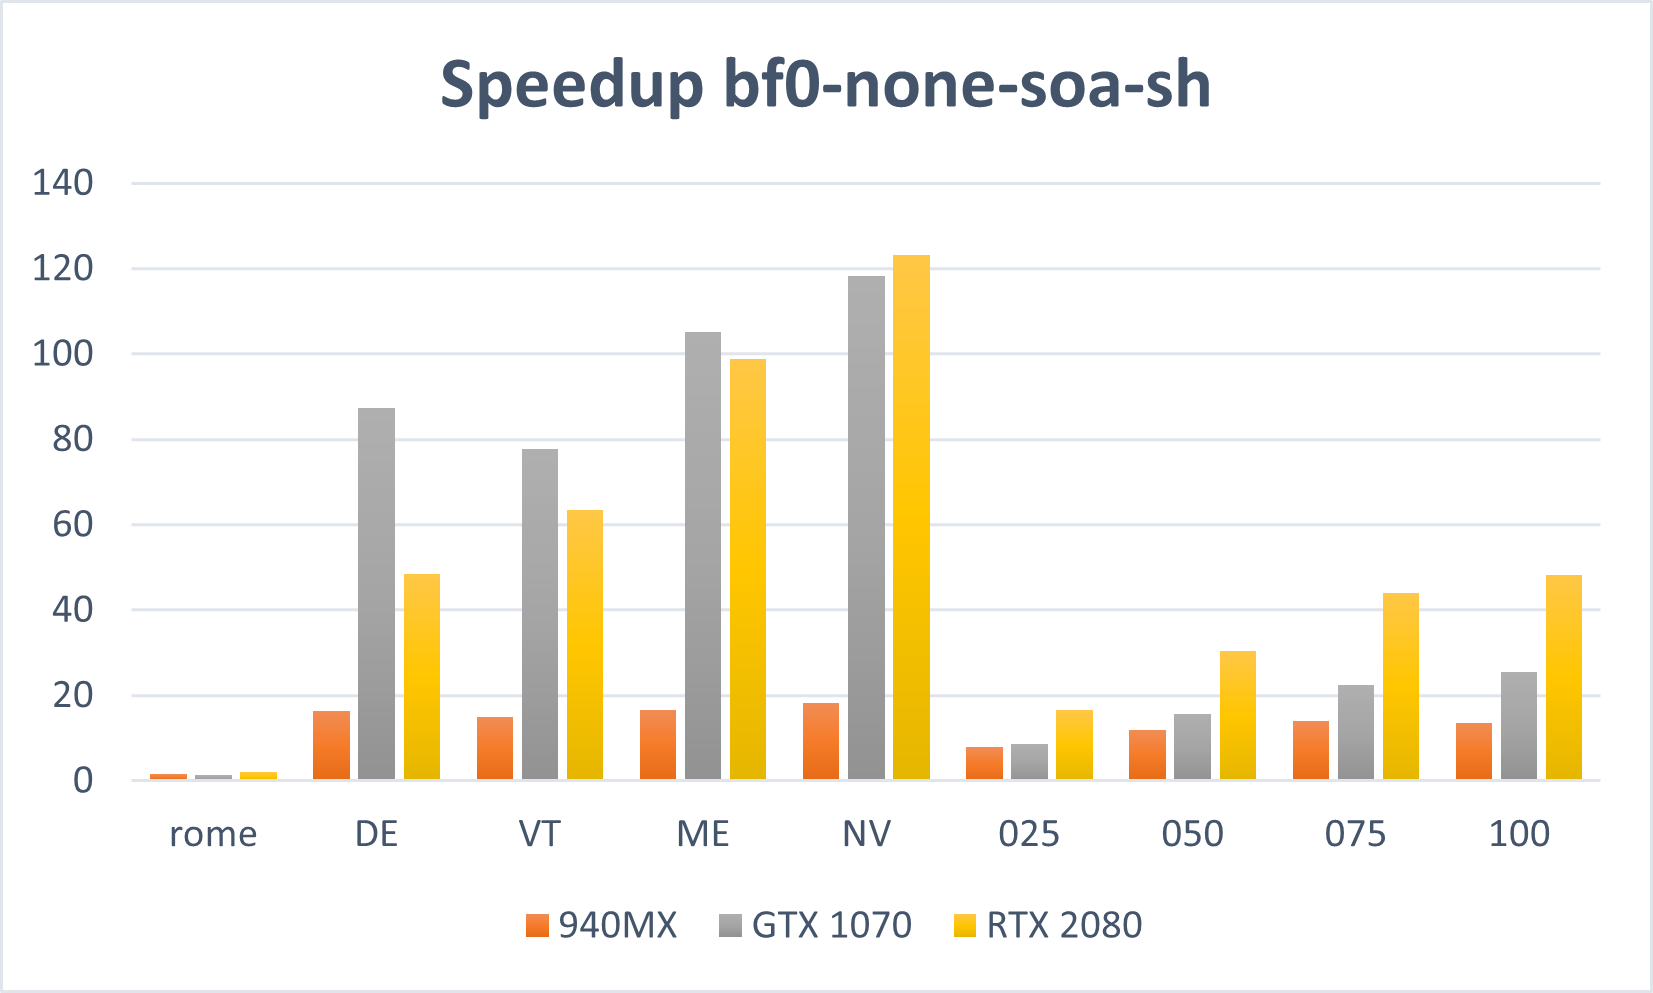
\includegraphics[width=\textwidth]{speedup_bf0-none-soa-sh}
		\end{subfigure}
		\caption{Speedup algoritmi \texttt{bf0-none}}
		\label{fig:speedup_bf0-none}
	\end{figure}

	\begin{figure}[b]
		\centering
		\begin{subfigure}{.5\textwidth}
			\centering
			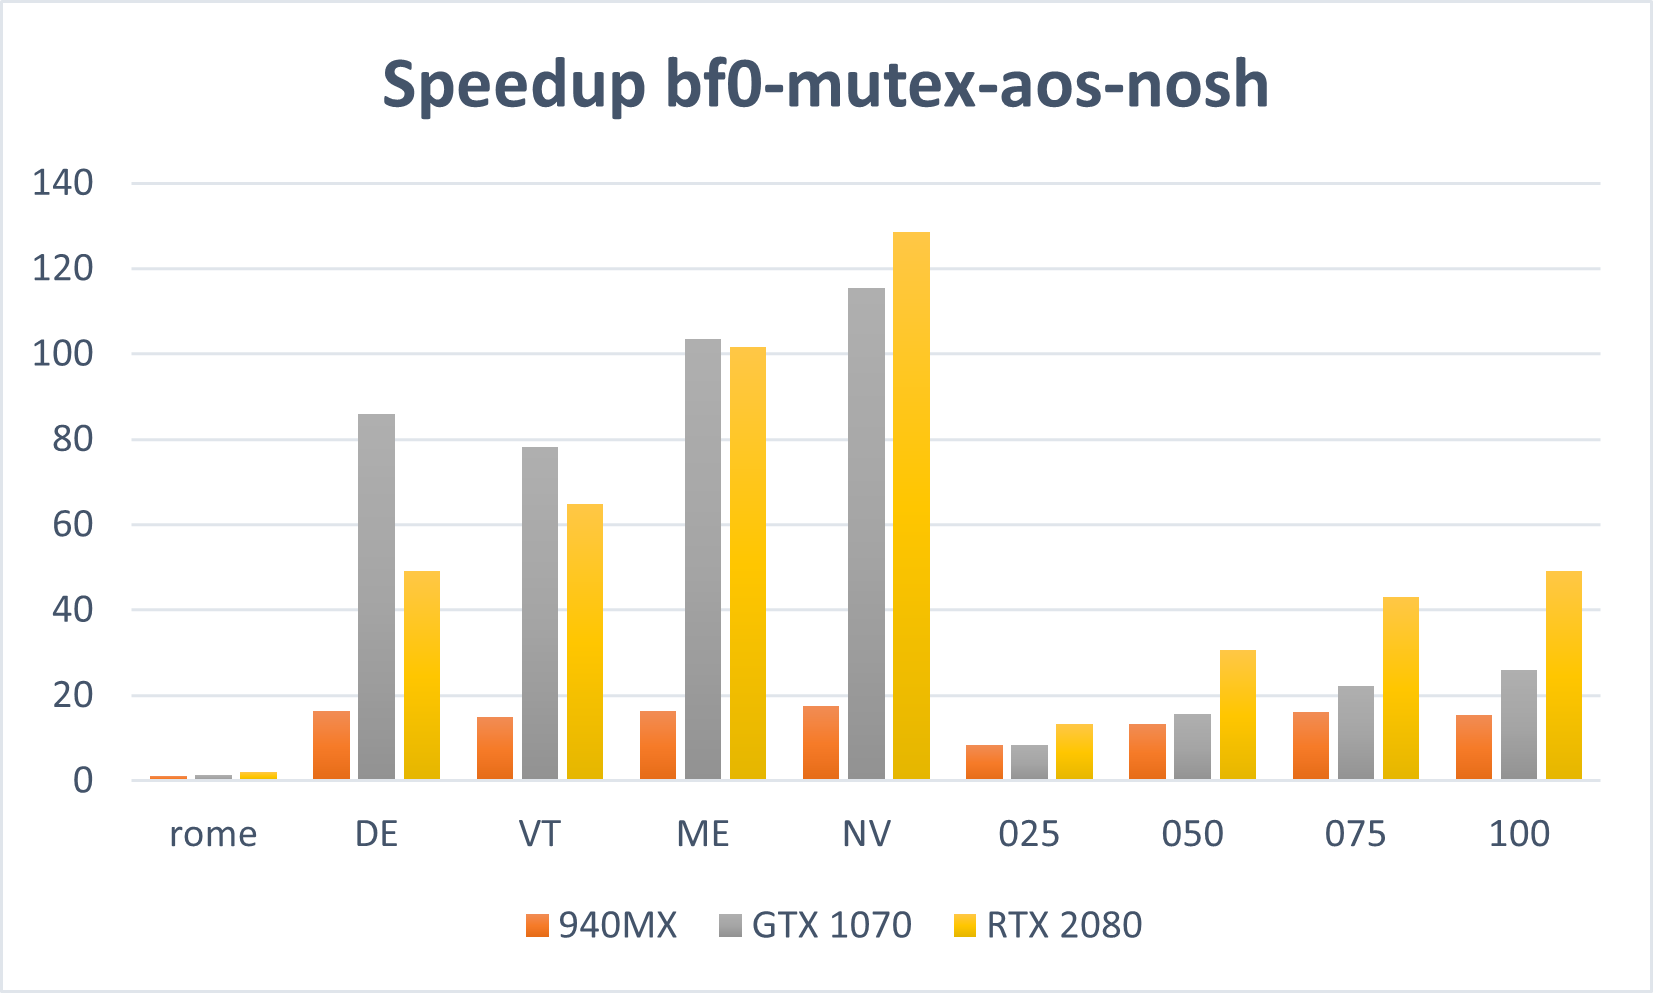
\includegraphics[width=\textwidth]{speedup_bf0-mutex-aos-nosh}
		\end{subfigure}%
		\begin{subfigure}{.5\textwidth}
			\centering
			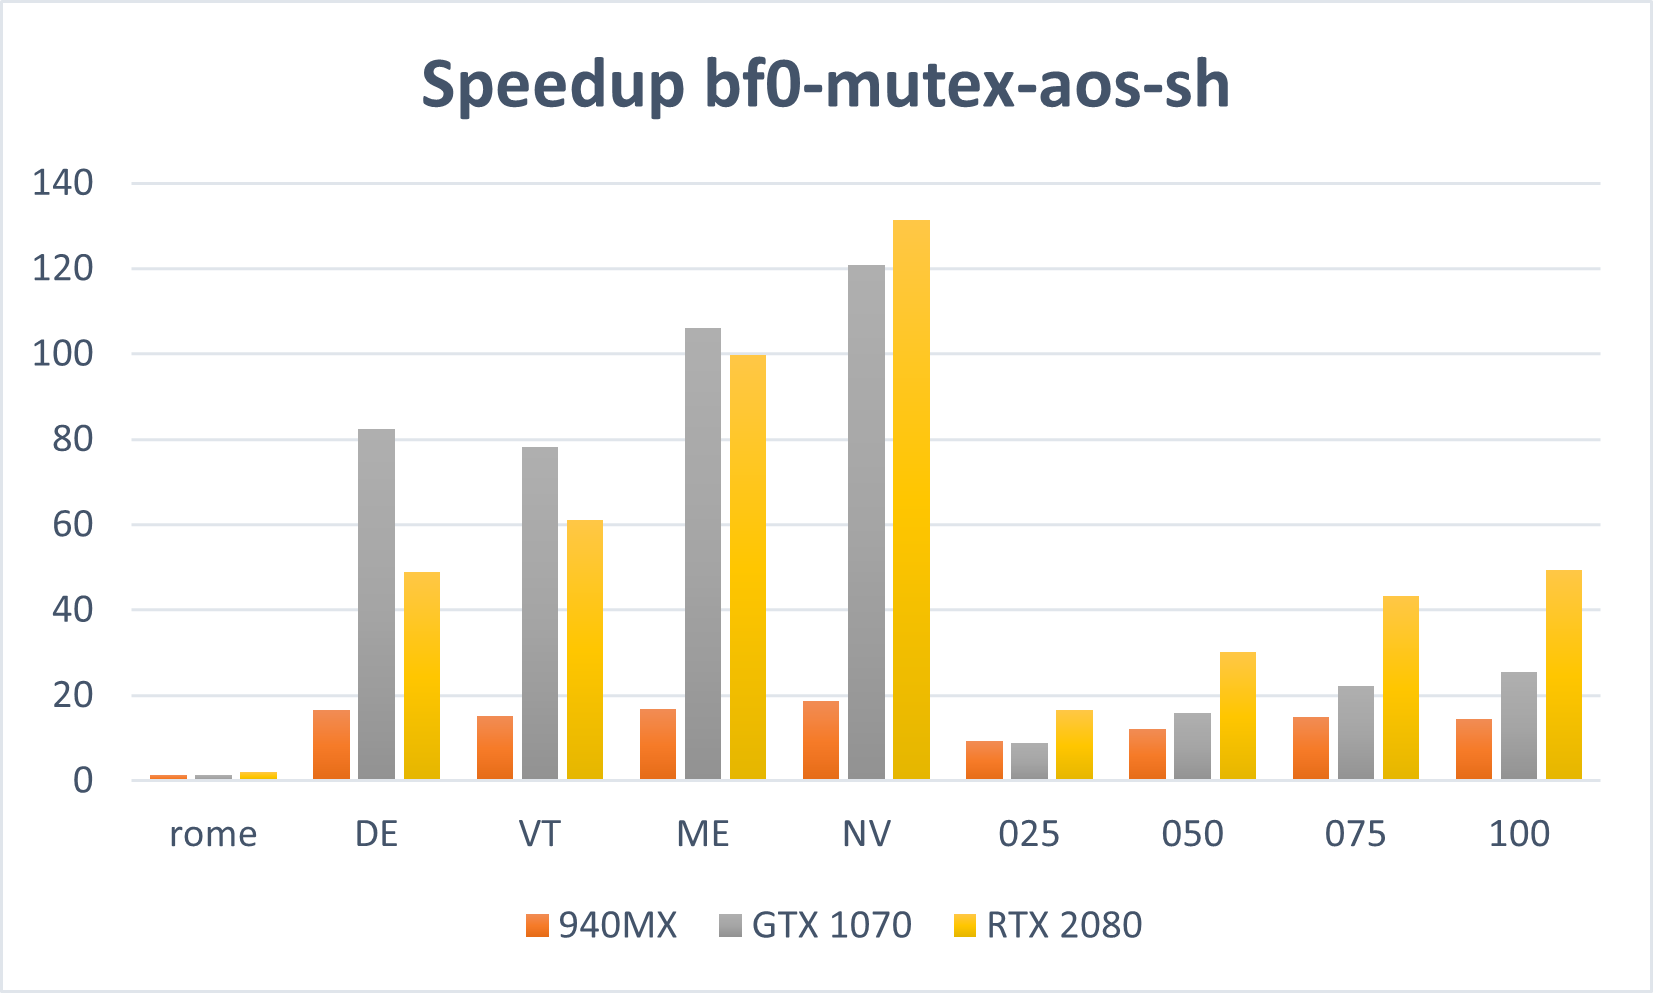
\includegraphics[width=\textwidth]{speedup_bf0-mutex-aos-sh}
		\end{subfigure}
		\begin{subfigure}{.5\textwidth}
			\centering
			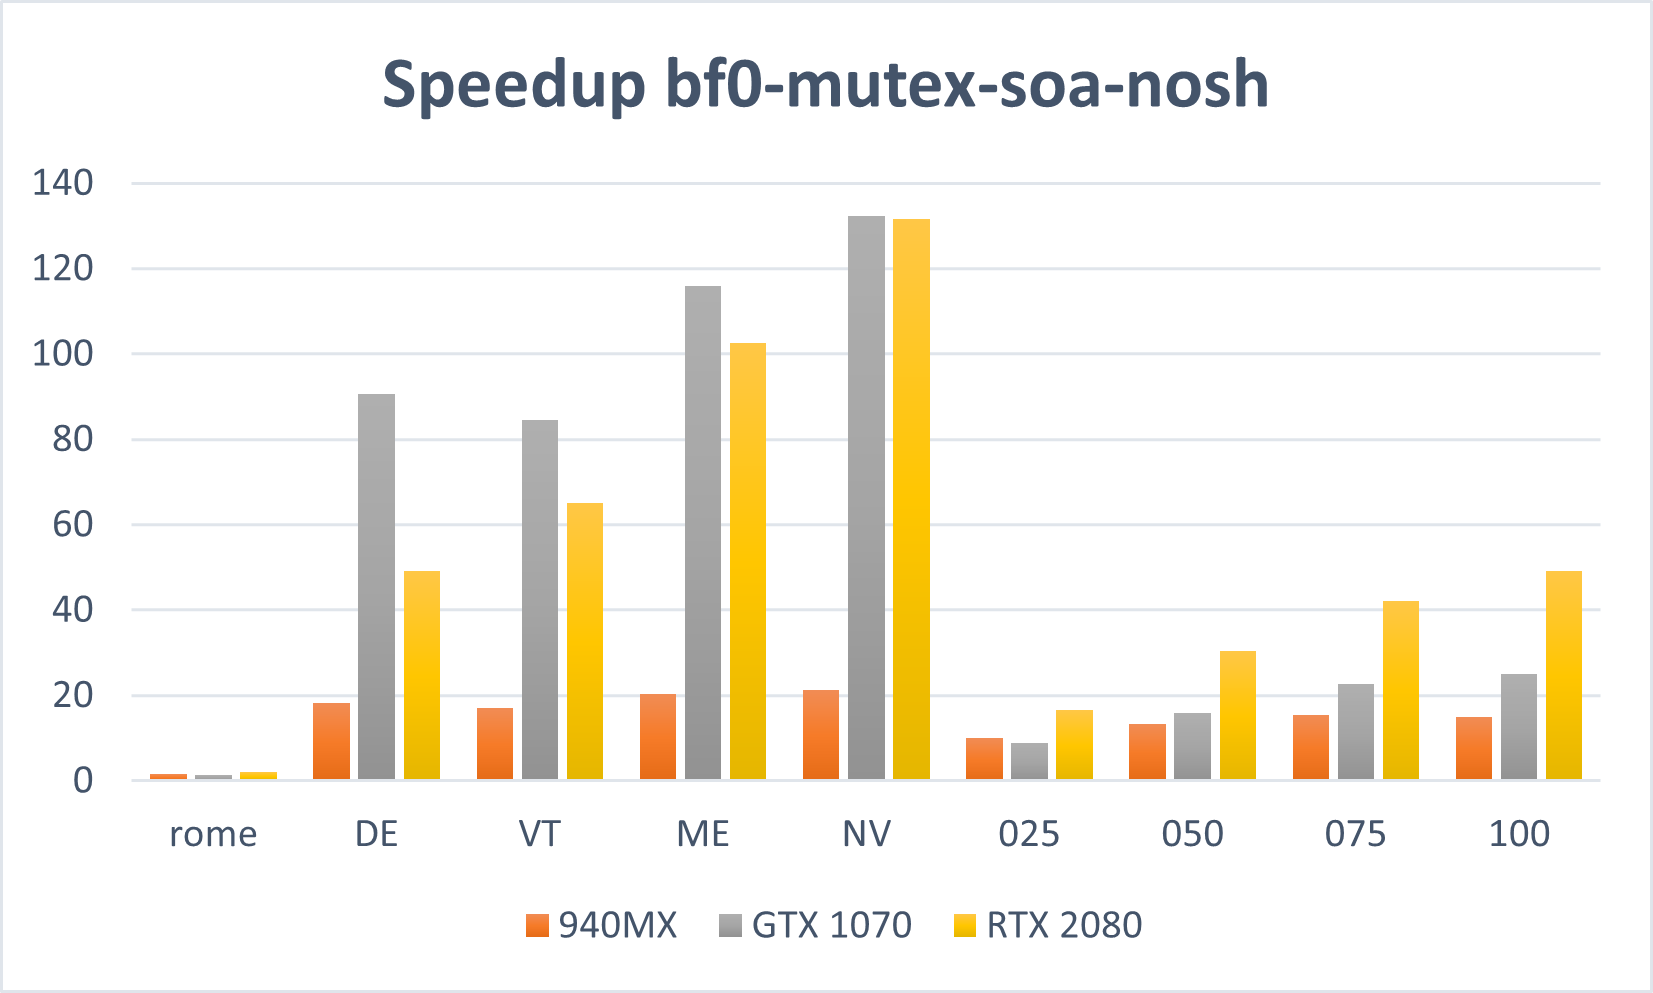
\includegraphics[width=\textwidth]{speedup_bf0-mutex-soa-nosh}
		\end{subfigure}%
		\begin{subfigure}{.5\textwidth}
			\centering
			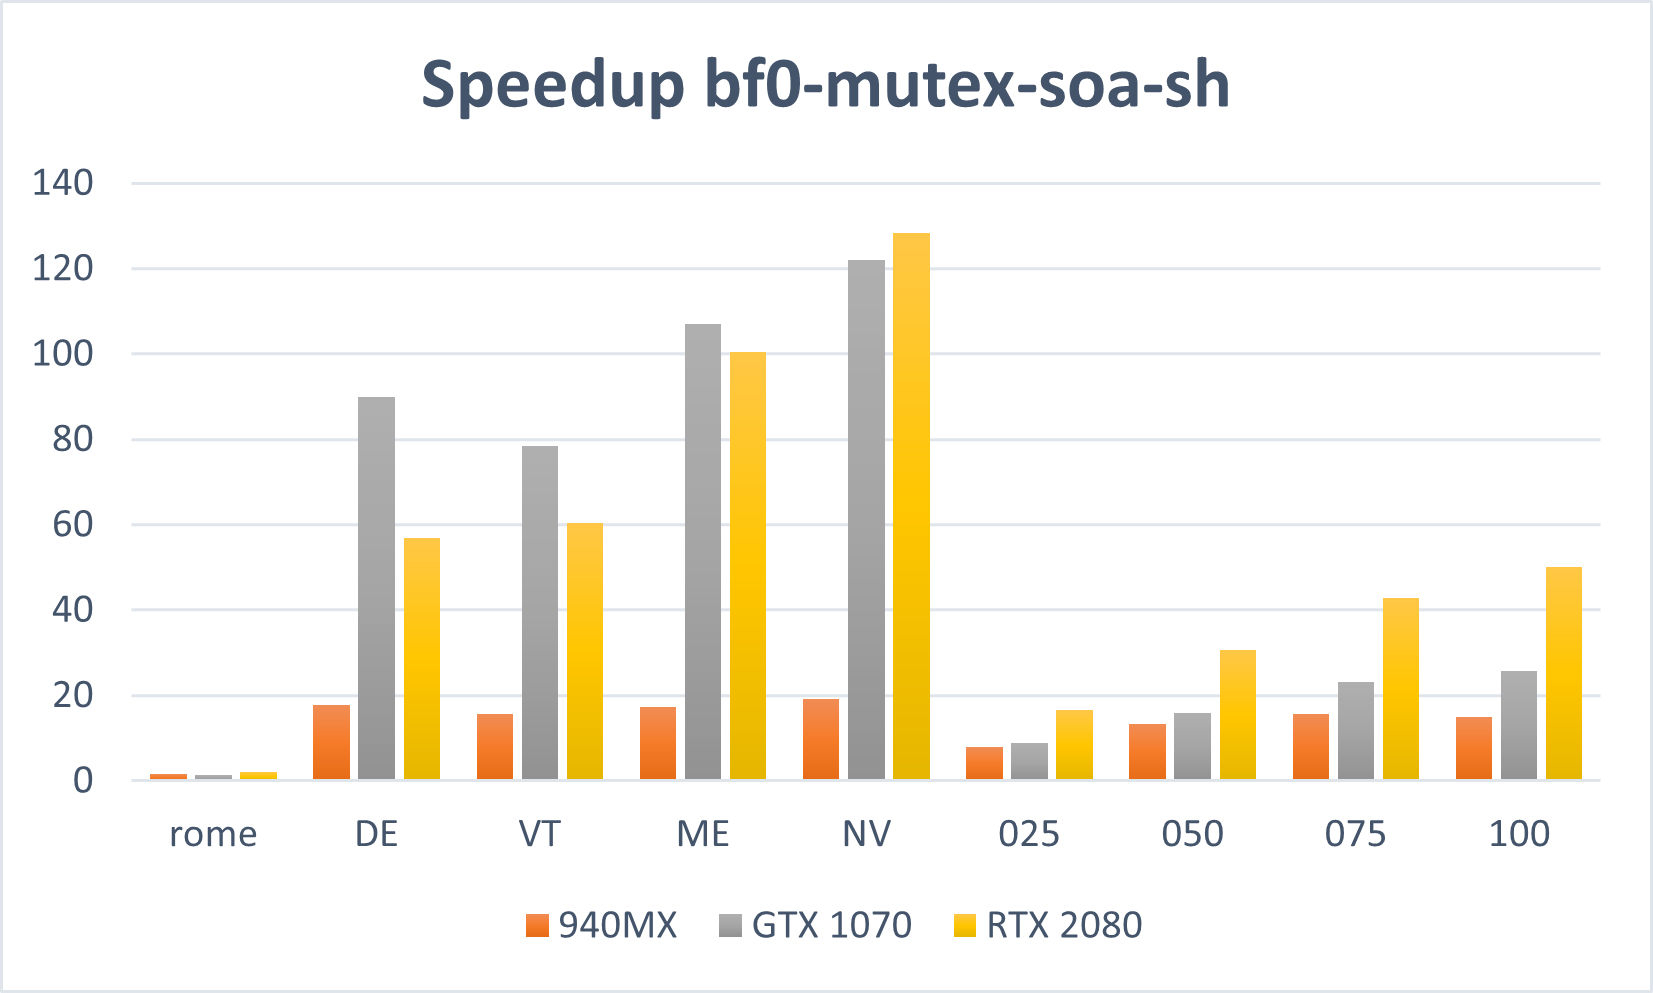
\includegraphics[width=\textwidth]{speedup_bf0-mutex-soa-sh}
		\end{subfigure}
		\caption{Speedup algoritmi \texttt{bf0-mutex}}
		\label{fig:speedup_bf0-mutex}
	\end{figure}

	Riguardo alle versioni \texttt{bf1}, invece, si nota subito dai grafici della figura \ref{fig:speedup_bf1} che la scala dello speedup ottenuto è molto più ridotta rispetto a quanto ottenuto con le versioni \texttt{bf0}. Infatti, solamente sui grafi sintetici si ottiene uno speedup significativo, mentre sui grafi "reali" lo speedup misurato è molto vicino allo $0$. Ciò era prevedibile a causa del ridottissimo numero di thread impiegati che, come già accennato nella sezione \ref{section:intro-bf1}, si sarebbero rivelati utili solamente su grafi molto piccoli e densi. Anche qui si osserva, in generale, un lieve miglioramento delle prestazioni grazie all'impiego della memoria condivisa e del pattern SoA.
	
	I valori misurati sui grafi \texttt{rome} e \texttt{DE} sono prossimi allo $0$.

	\begin{figure}[b]
		\centering
		\begin{subfigure}{.5\textwidth}
			\centering
			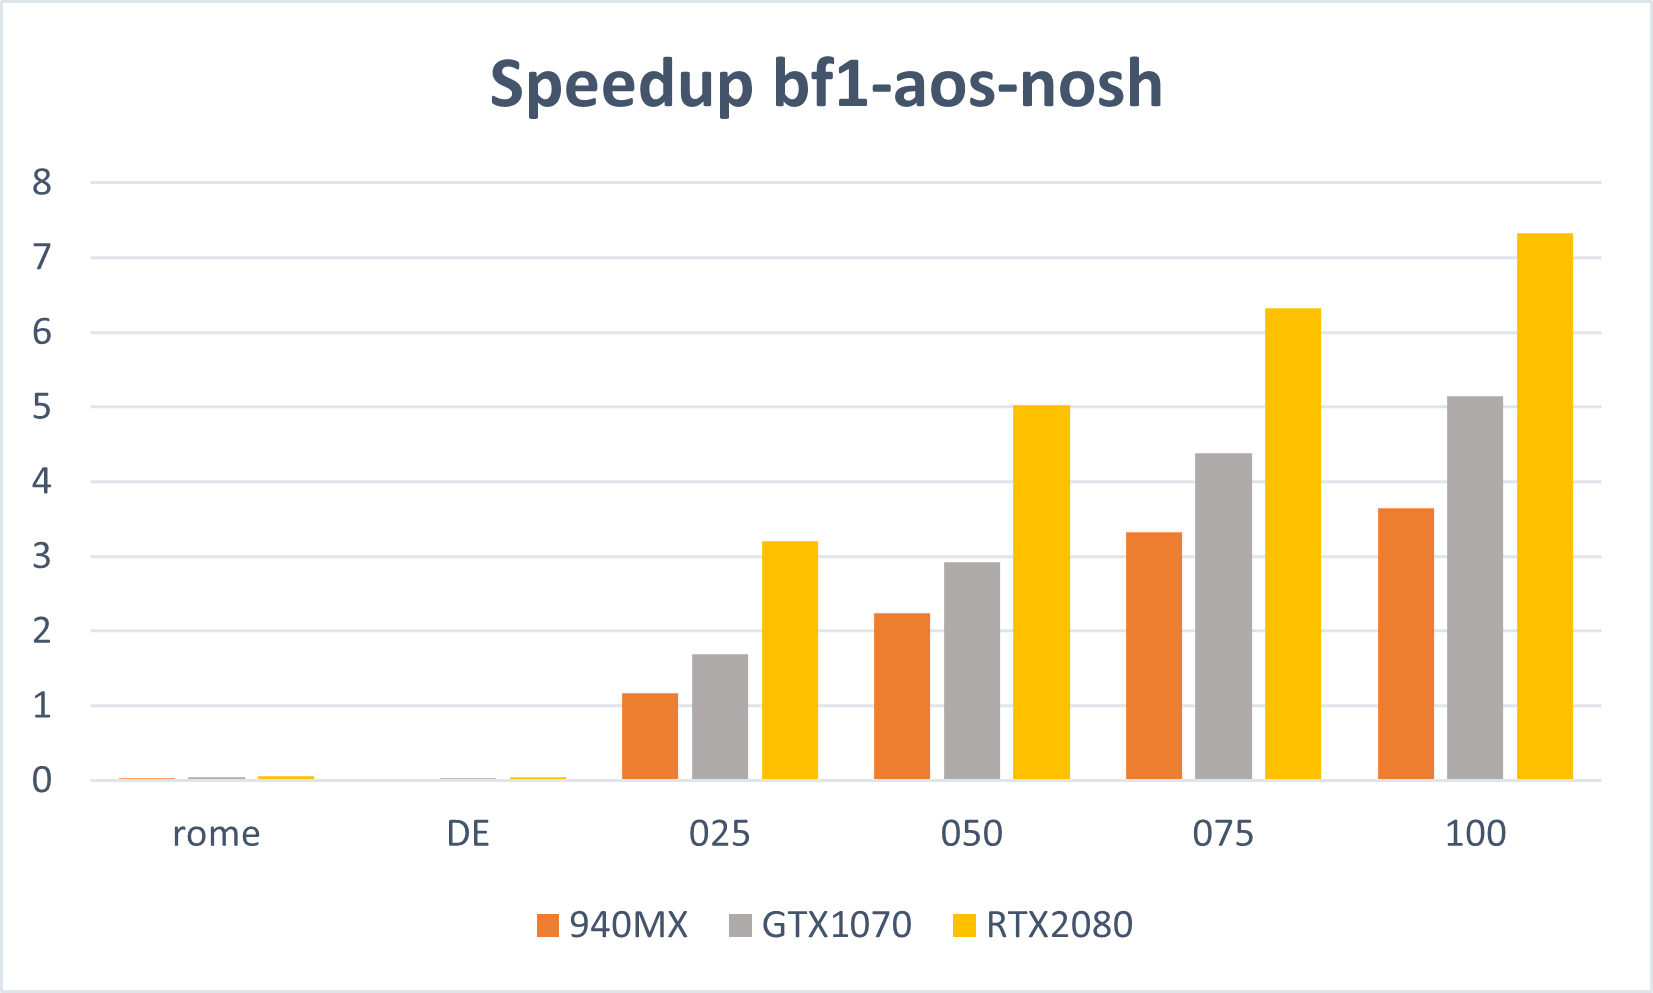
\includegraphics[width=\textwidth]{speedup_bf1-aos-nosh}
		\end{subfigure}%
		\begin{subfigure}{.5\textwidth}
			\centering
			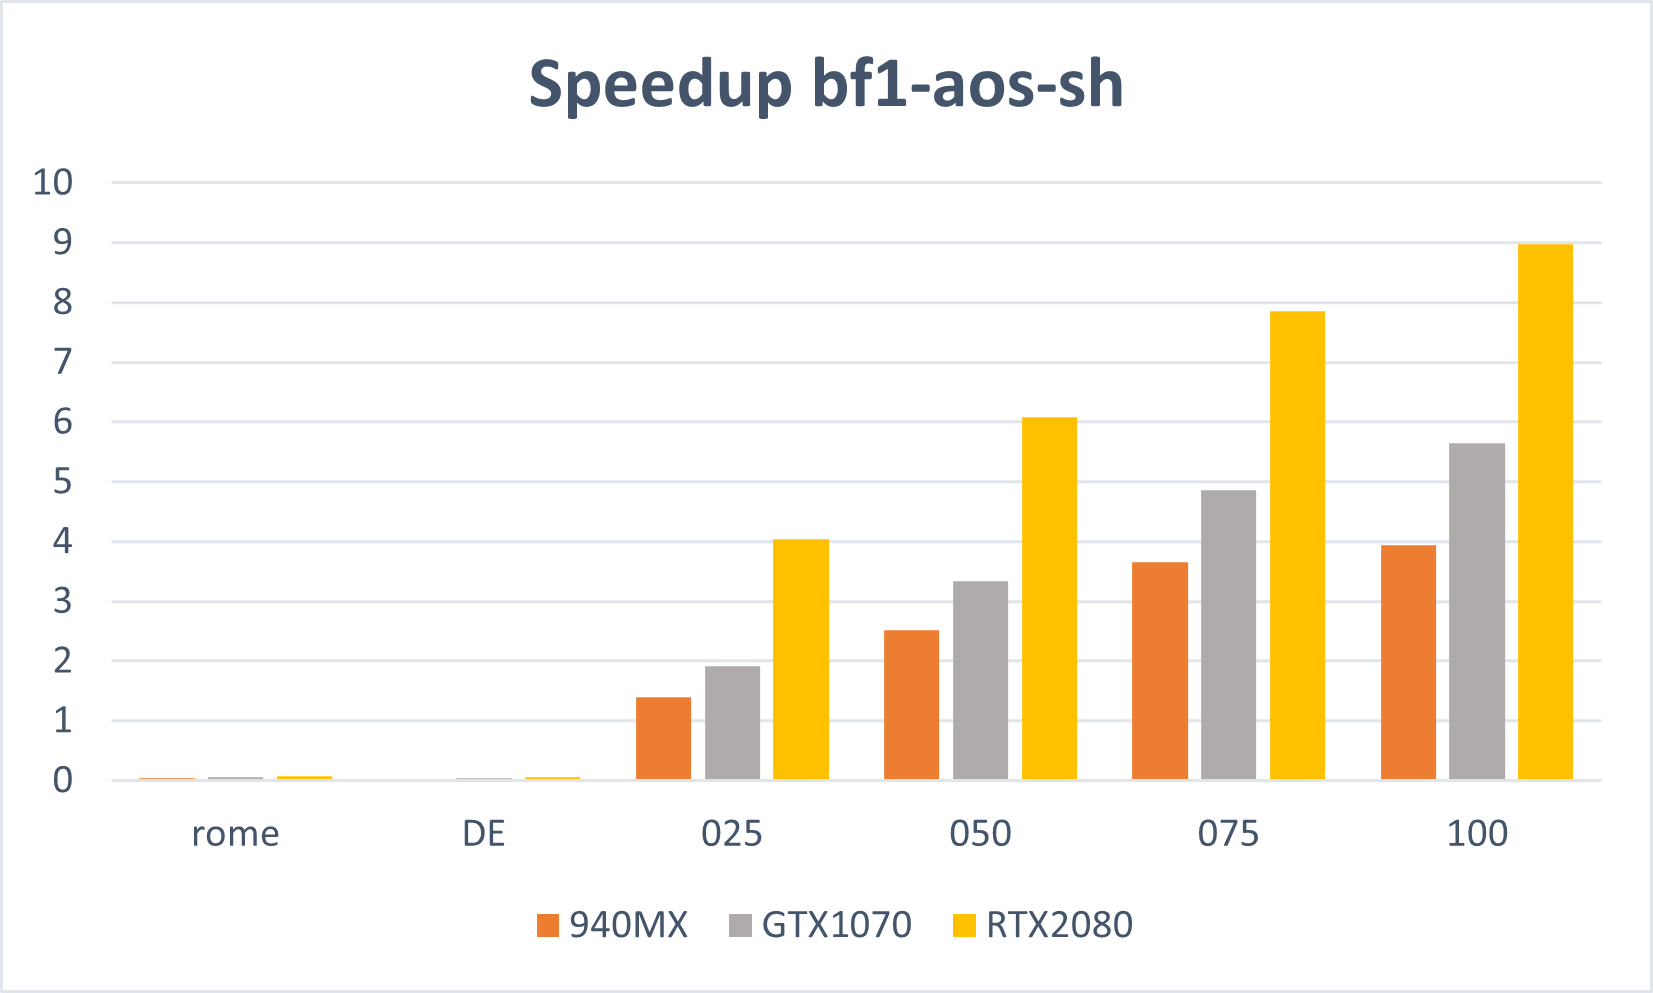
\includegraphics[width=\textwidth]{speedup_bf1-aos-sh}
		\end{subfigure}
		\begin{subfigure}{.5\textwidth}
			\centering
			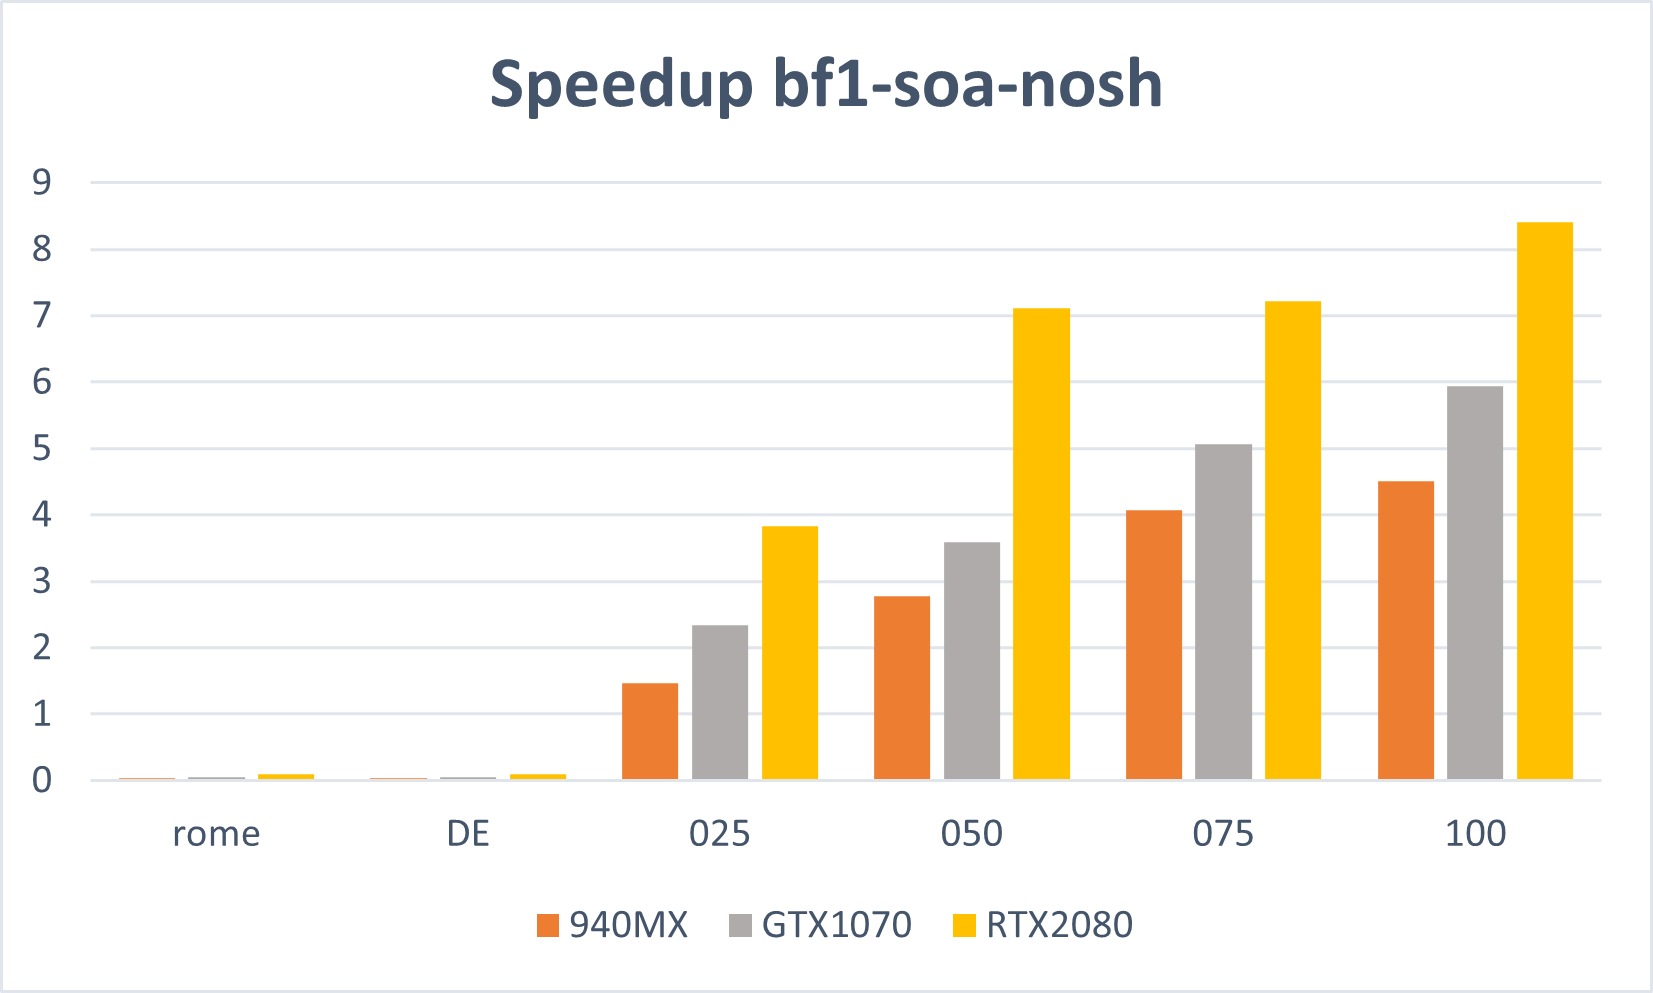
\includegraphics[width=\textwidth]{speedup_bf1-soa-nosh}
		\end{subfigure}%
		\begin{subfigure}{.5\textwidth}
			\centering
			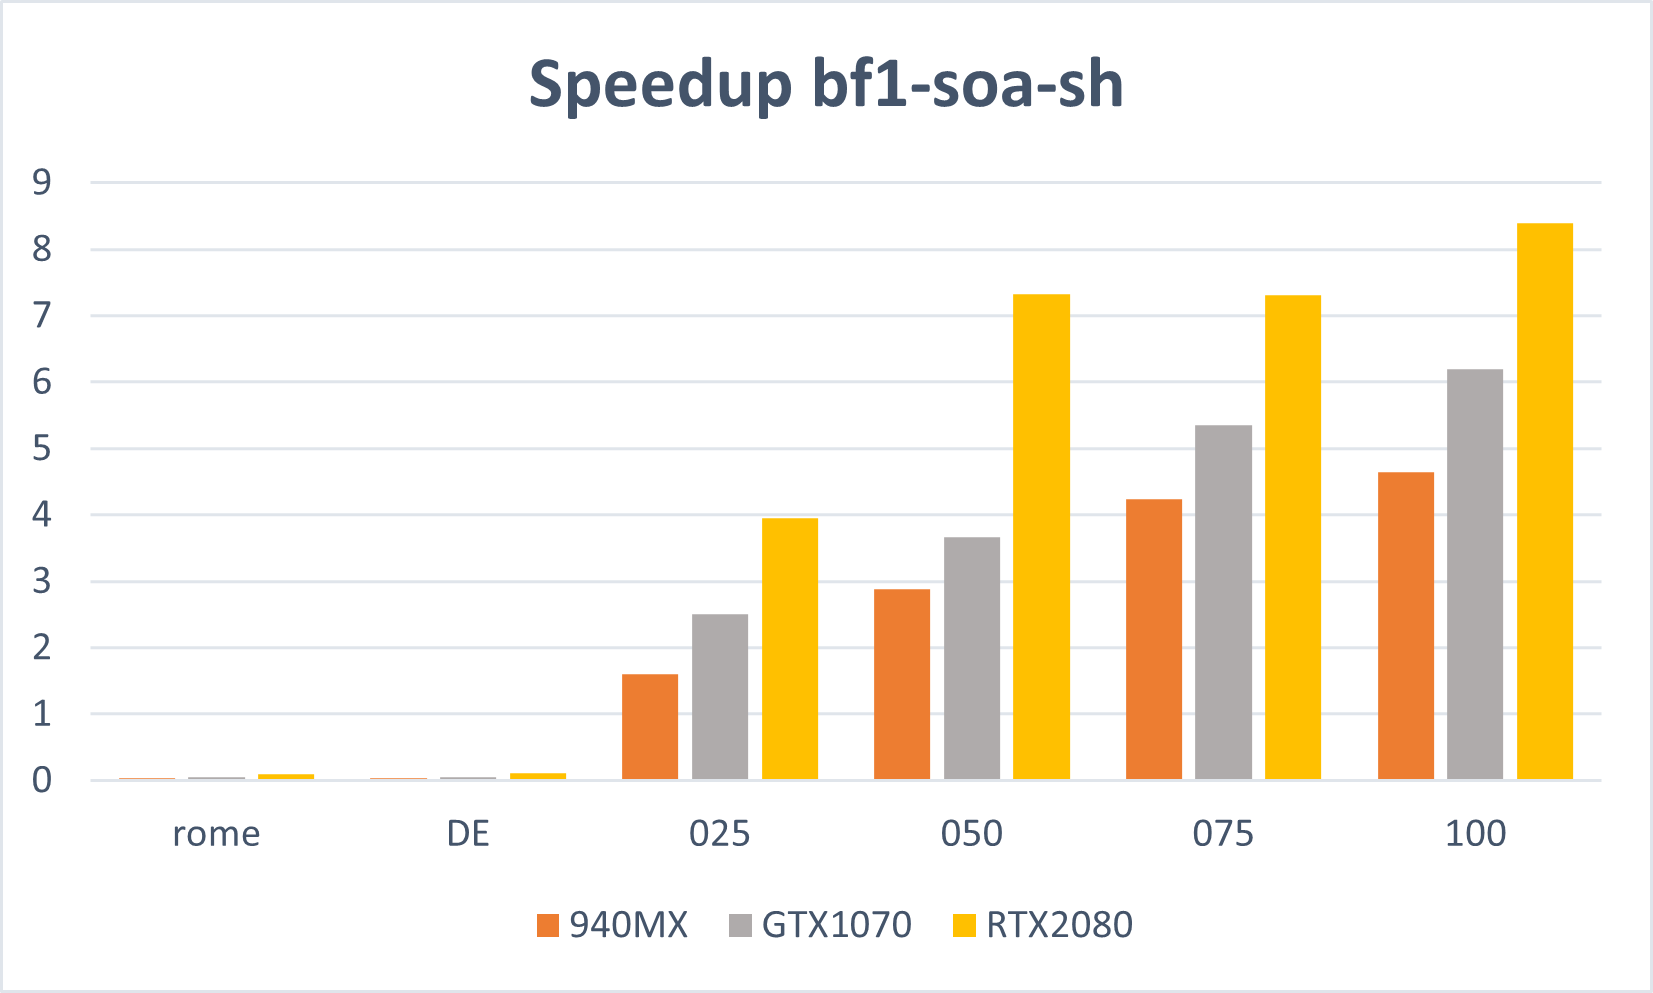
\includegraphics[width=\textwidth]{speedup_bf1-soa-sh}
		\end{subfigure}
		\caption{Speedup algoritmi \texttt{bf1}}
		\label{fig:speedup_bf1}
	\end{figure}

	Infine con le versioni \texttt{bf2} si notano valori di speedup decisamente più alti rispetto alle versioni \texttt{bf1}, ma solamente sui grafi sintetici. Nella figura \ref{fig:speedup_bf2}, si può notare che sugli altri grafi sono stati registrati valori intorno ad $1$ e quindi non significativi. Questa grande differenza rispecchia perfettamente la struttura degli algoritmi \texttt{bf2}: utilizzando solamente $1024$ thread per rilassare gli archi entranti di ogni nodo l'incremento di prestazioni diventa significativo solamente su grafi con elevata densità. Va notato, però, che l'unica versione che impiega SoA riporta valori di speedup molto più elevati rispetto alle due versioni \texttt{bf2-aos}.

	\begin{figure}[b]
		\centering
		\begin{subfigure}{.5\textwidth}
			\centering
			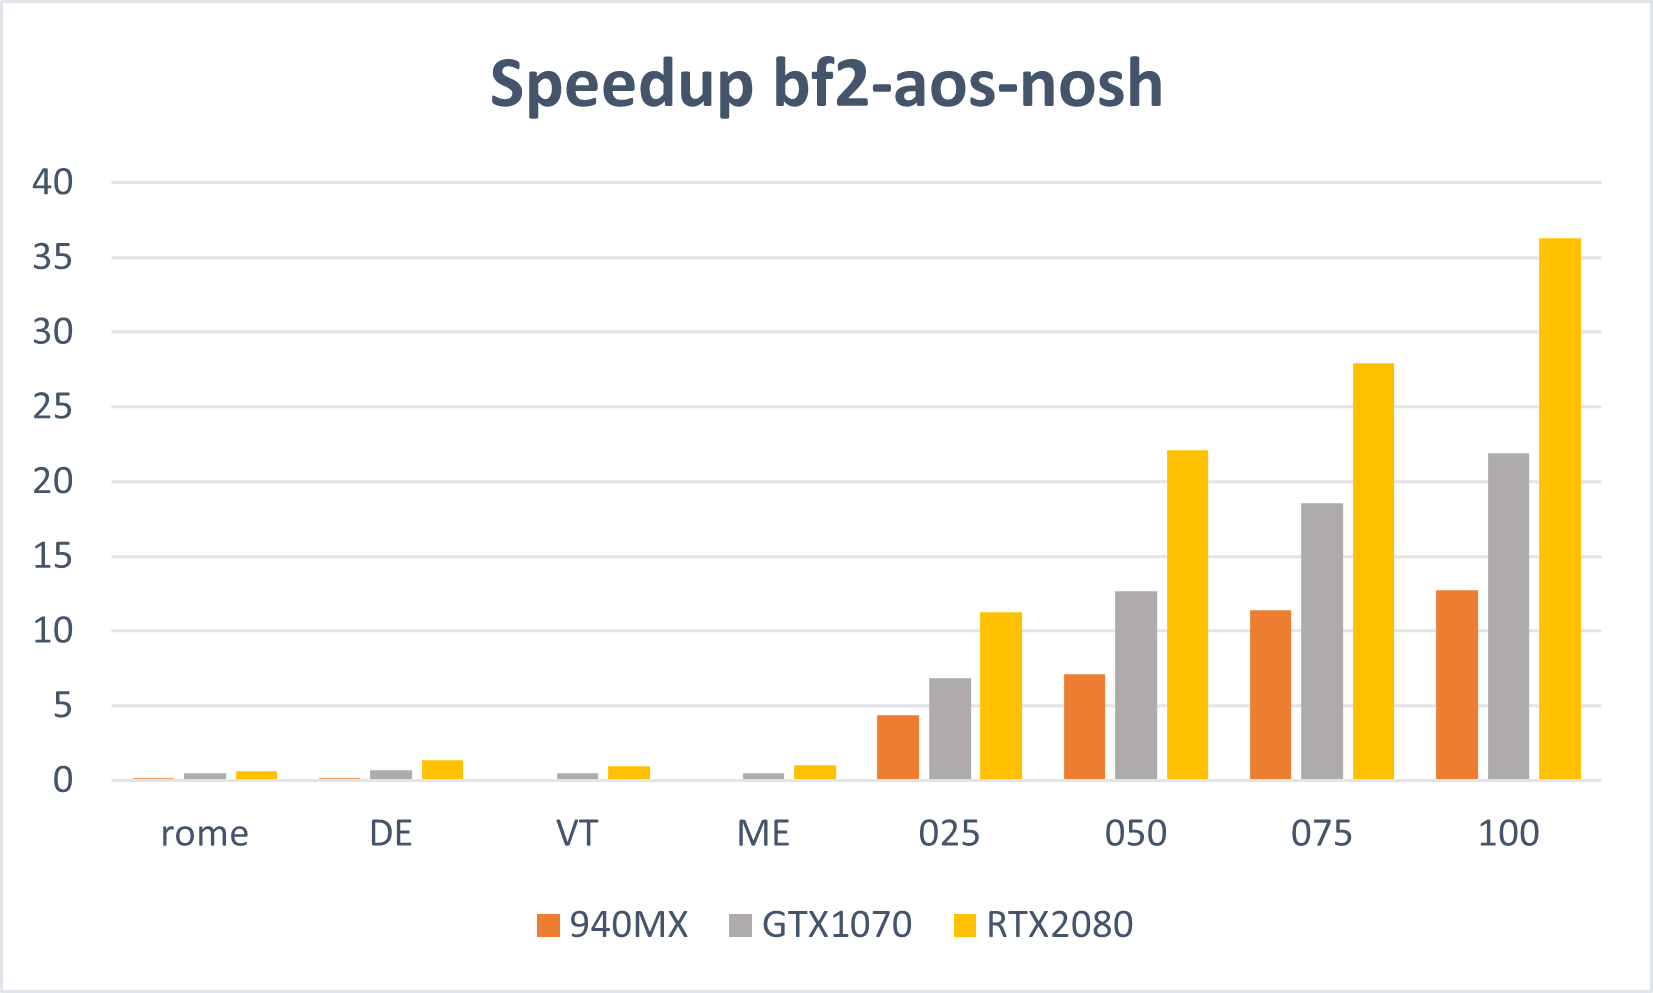
\includegraphics[width=\textwidth]{speedup_bf2-aos-nosh}
		\end{subfigure}%
		\begin{subfigure}{.5\textwidth}
			\centering
			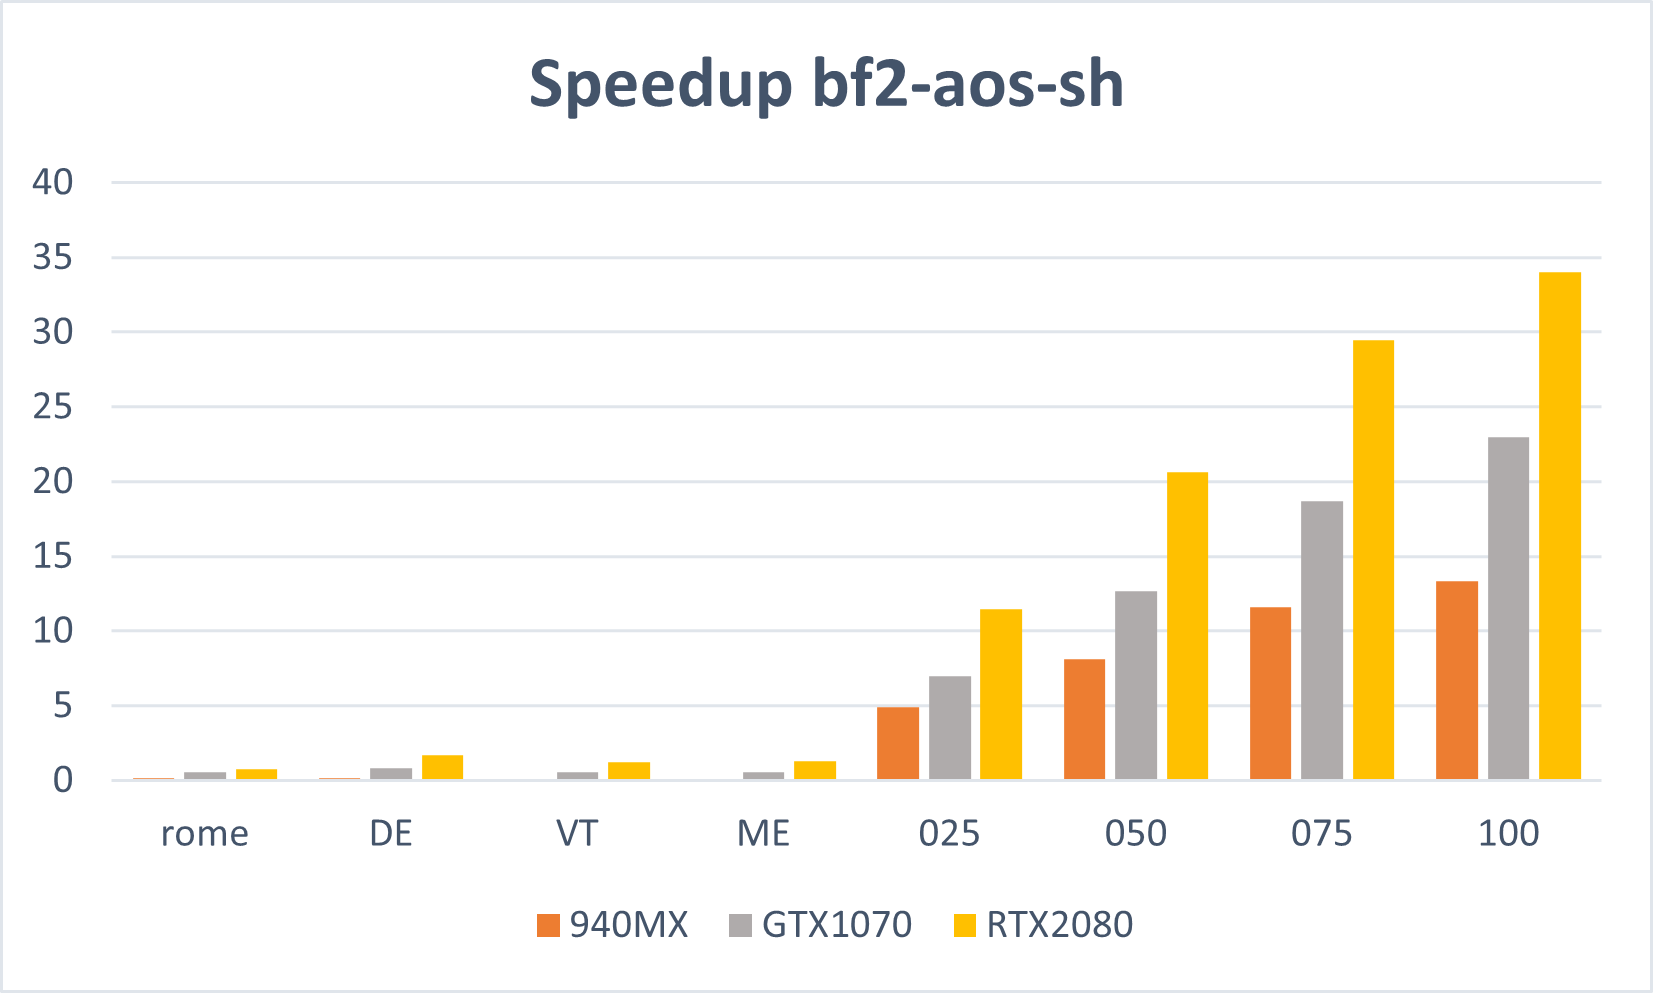
\includegraphics[width=\textwidth]{speedup_bf2-aos-sh}
		\end{subfigure}
		\begin{subfigure}{.5\textwidth}
			\centering
			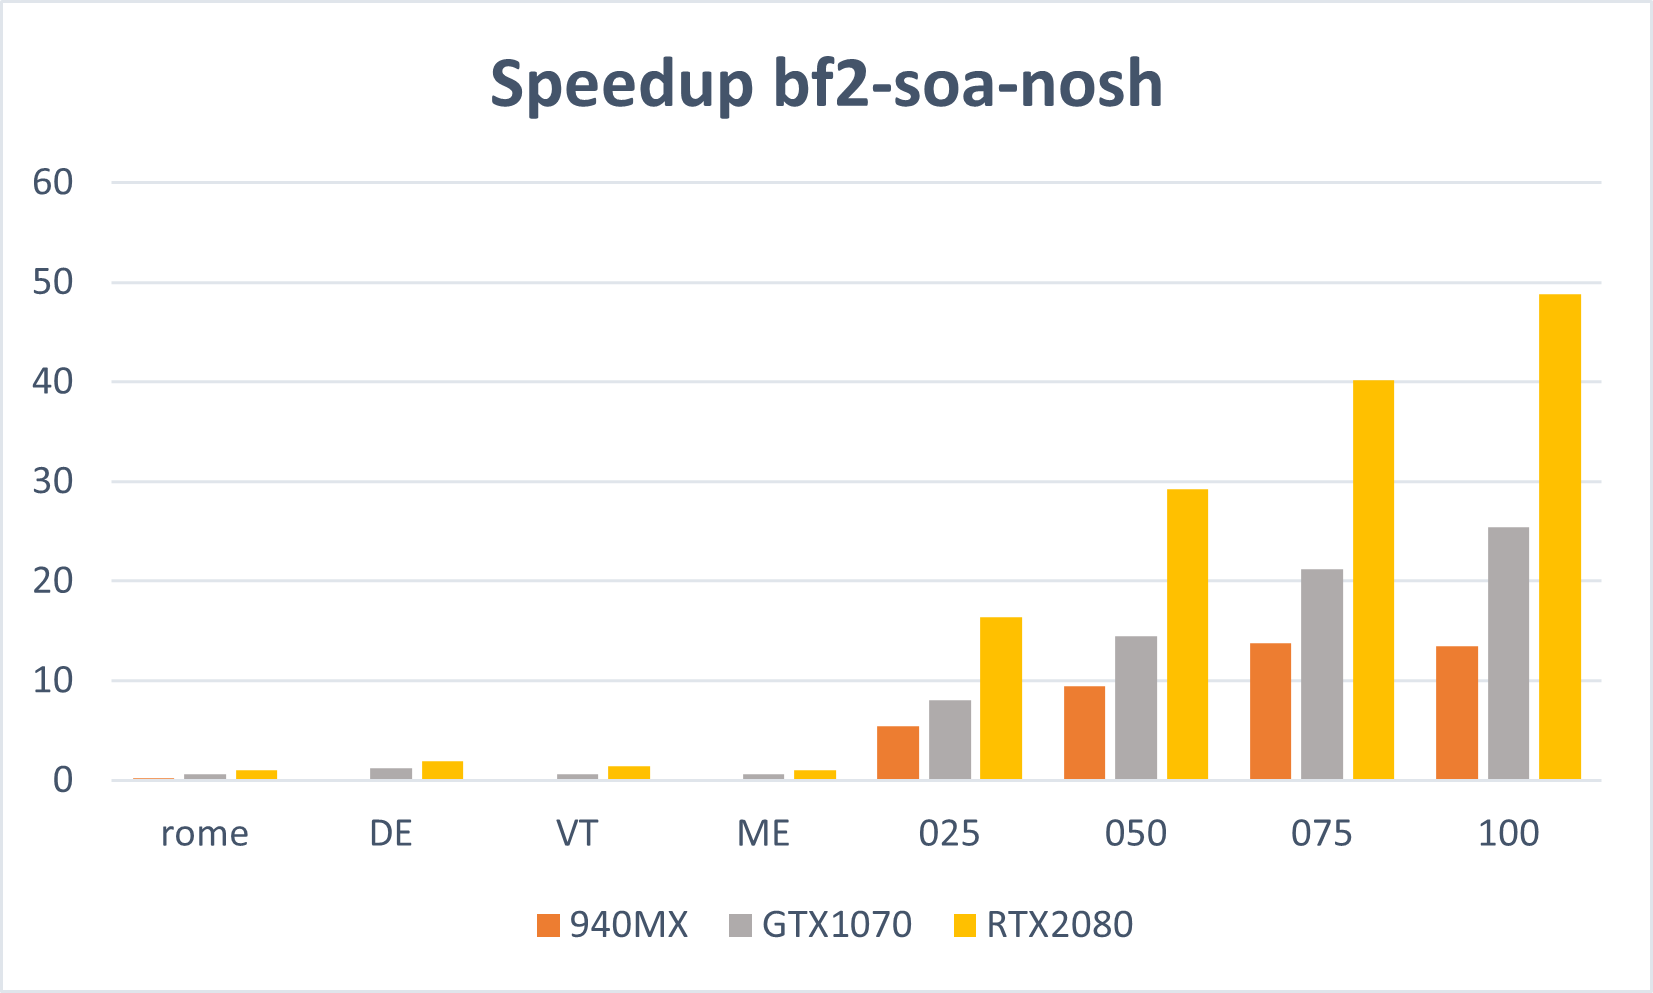
\includegraphics[width=\textwidth]{speedup_bf2-soa-nosh}
		\end{subfigure}%
		\caption{Speedup algoritmi \texttt{bf2}}
		\label{fig:speedup_bf2}
	\end{figure}
	
	\section{Throughput}
	Di seguito sono riportati i valori di throughput di ogni versione, misurati sui test a disposizione e su ogni scheda, indicati in milioni di operazioni di rilassamento effettuate ogni secondo ($10^6$ relax/s).
	
	Come già spiegato più sopra per lo speedup, nelle figure \ref{fig:throughput_bf0-none} e \ref{fig:throughput_bf0-mutex} si nota l'enorme differenza tra la scheda 940MX e le altre. \'E comunque interessante notare come i valori della scheda GTX1070, pur sempre elevati, risultino meno variabili di quelli misurati sulla scheda RTX2080.
	
	I valori misurati sul grafo \texttt{rome}, come per lo speedup, risultano di almeno due ordini di grandezza minori rispetto ai valori misurati sugli altri test.
	
	\begin{figure}[b]
		\centering
		\begin{subfigure}{.5\textwidth}
			\centering
			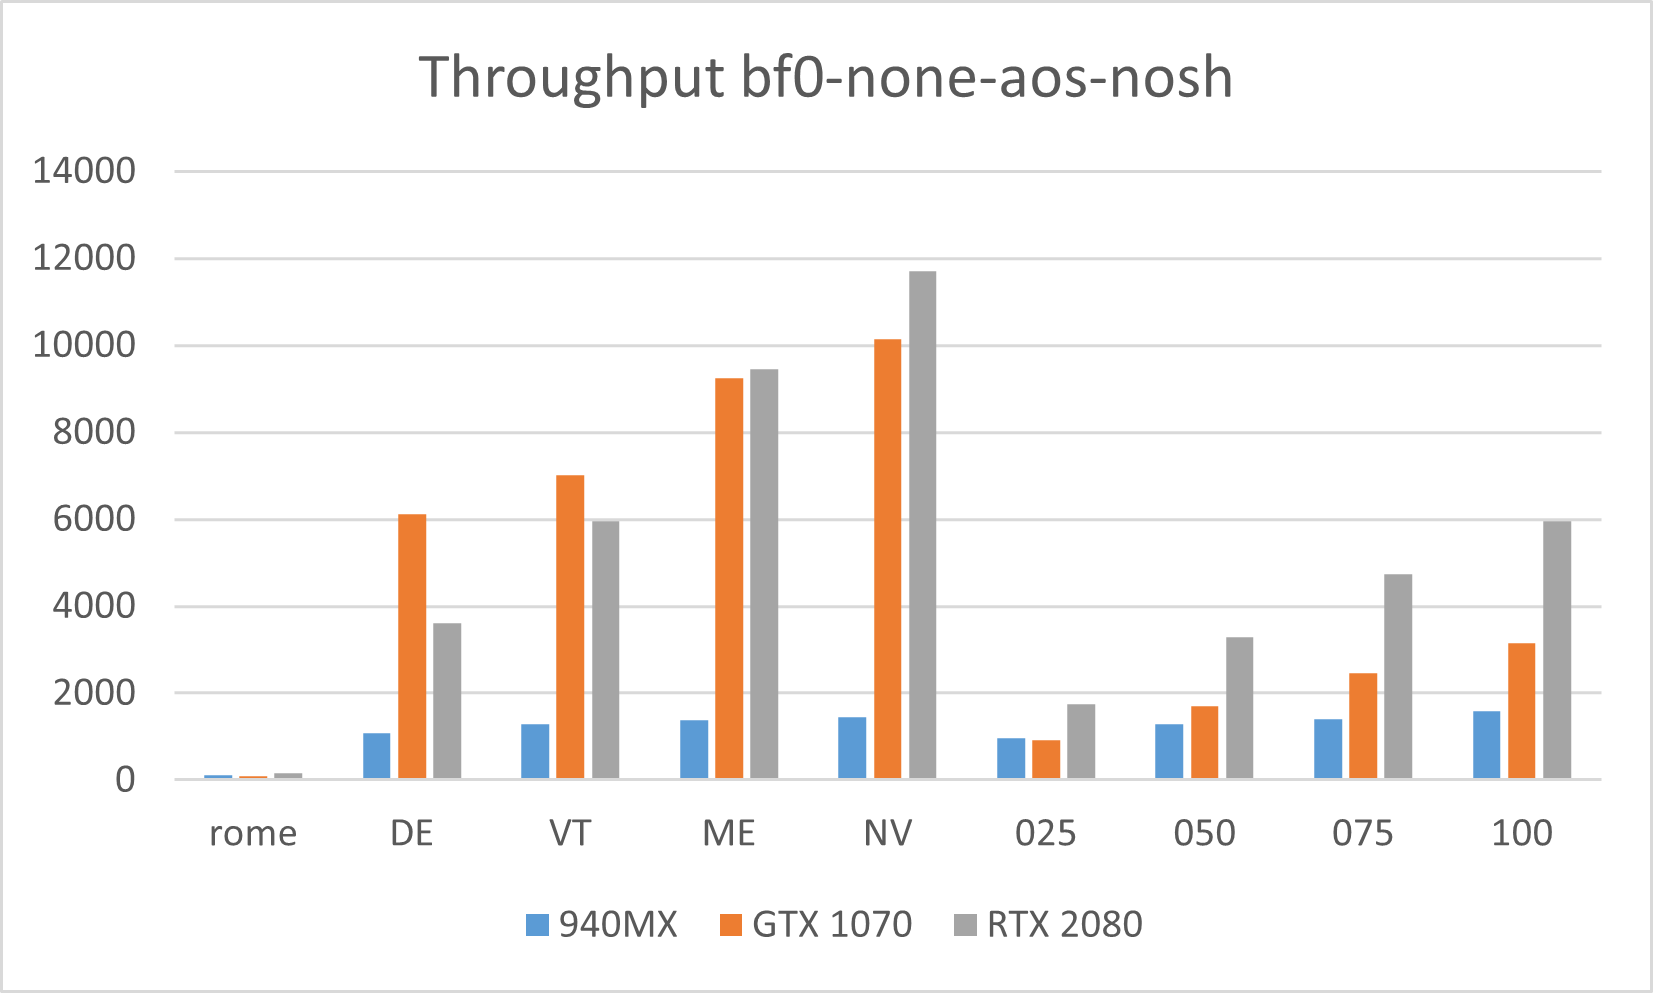
\includegraphics[width=\textwidth]{throughput_bf0-none-aos-nosh}
		\end{subfigure}%
		\begin{subfigure}{.5\textwidth}
			\centering
			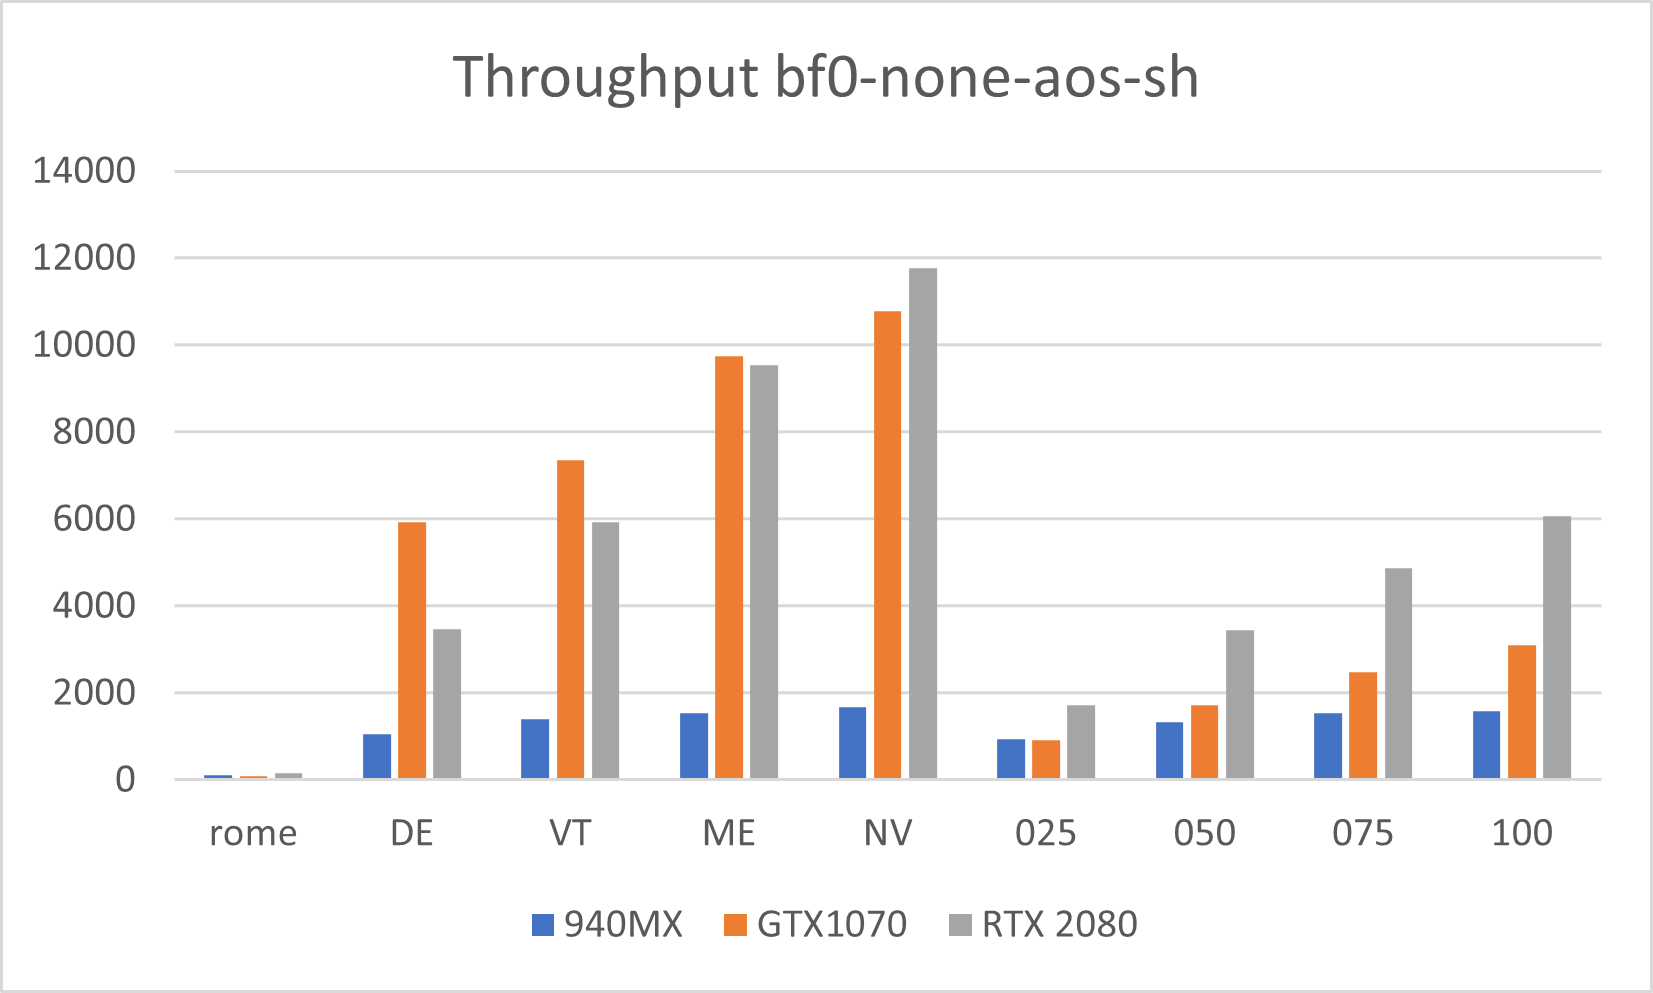
\includegraphics[width=\textwidth]{throughput_bf0-none-aos-sh}
		\end{subfigure}
		\begin{subfigure}{.5\textwidth}
			\centering
			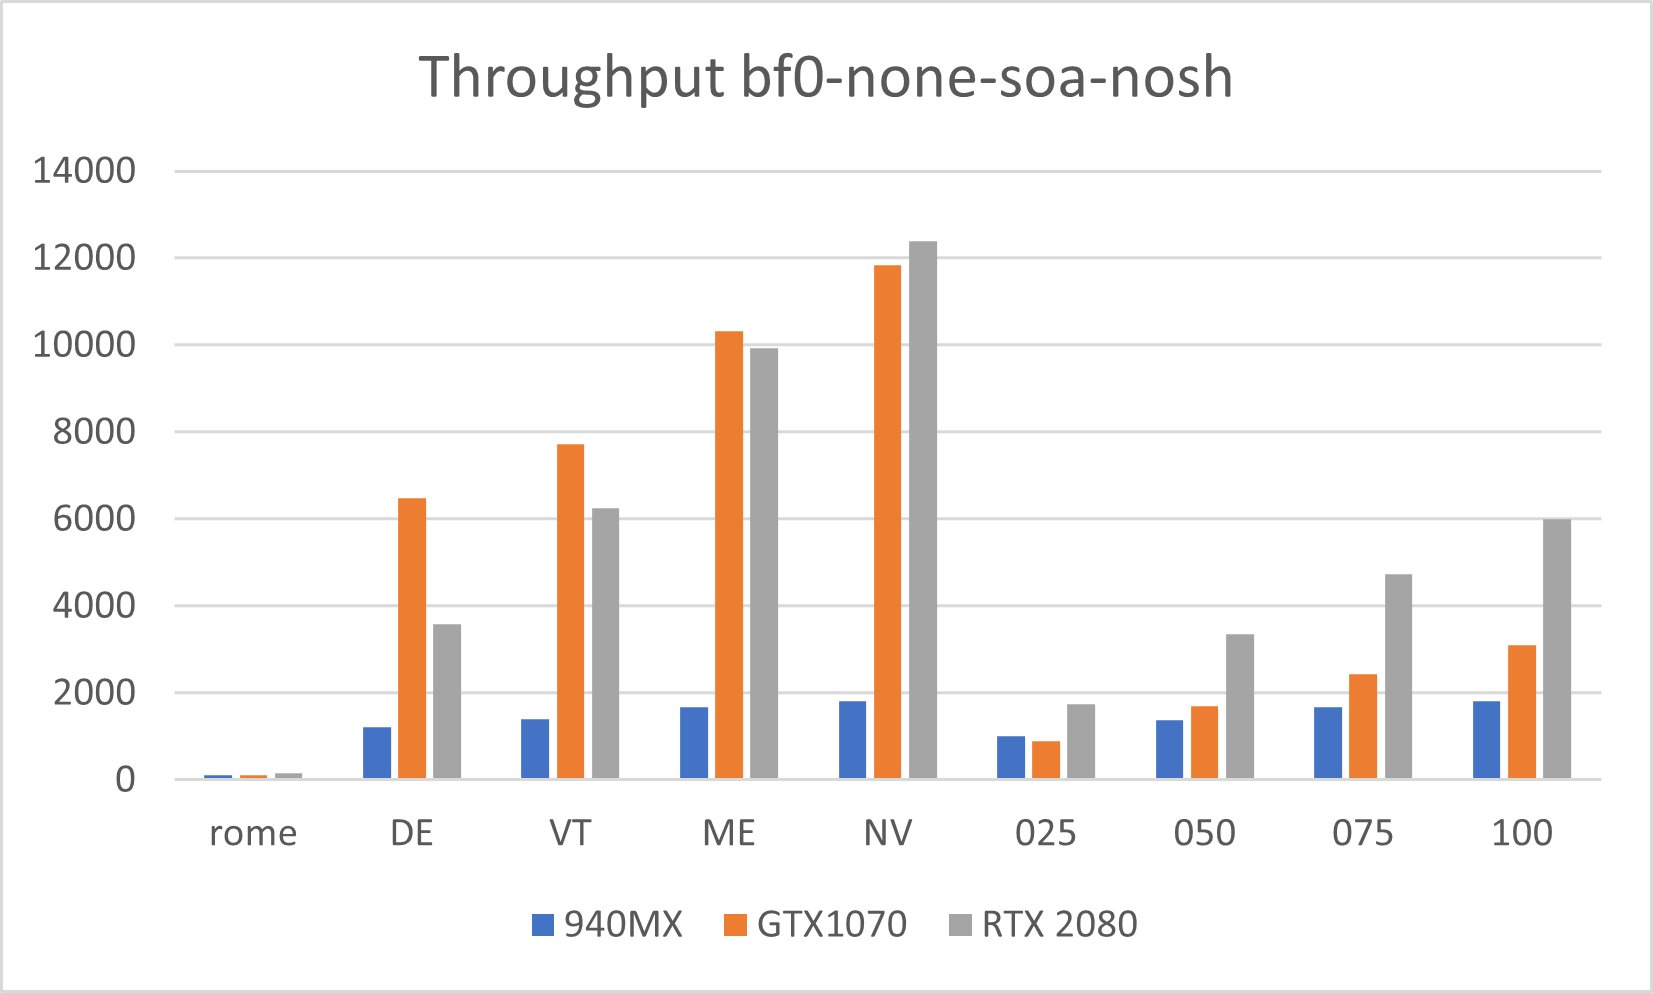
\includegraphics[width=\textwidth]{throughput_bf0-none-soa-nosh}
		\end{subfigure}%
		\begin{subfigure}{.5\textwidth}
			\centering
			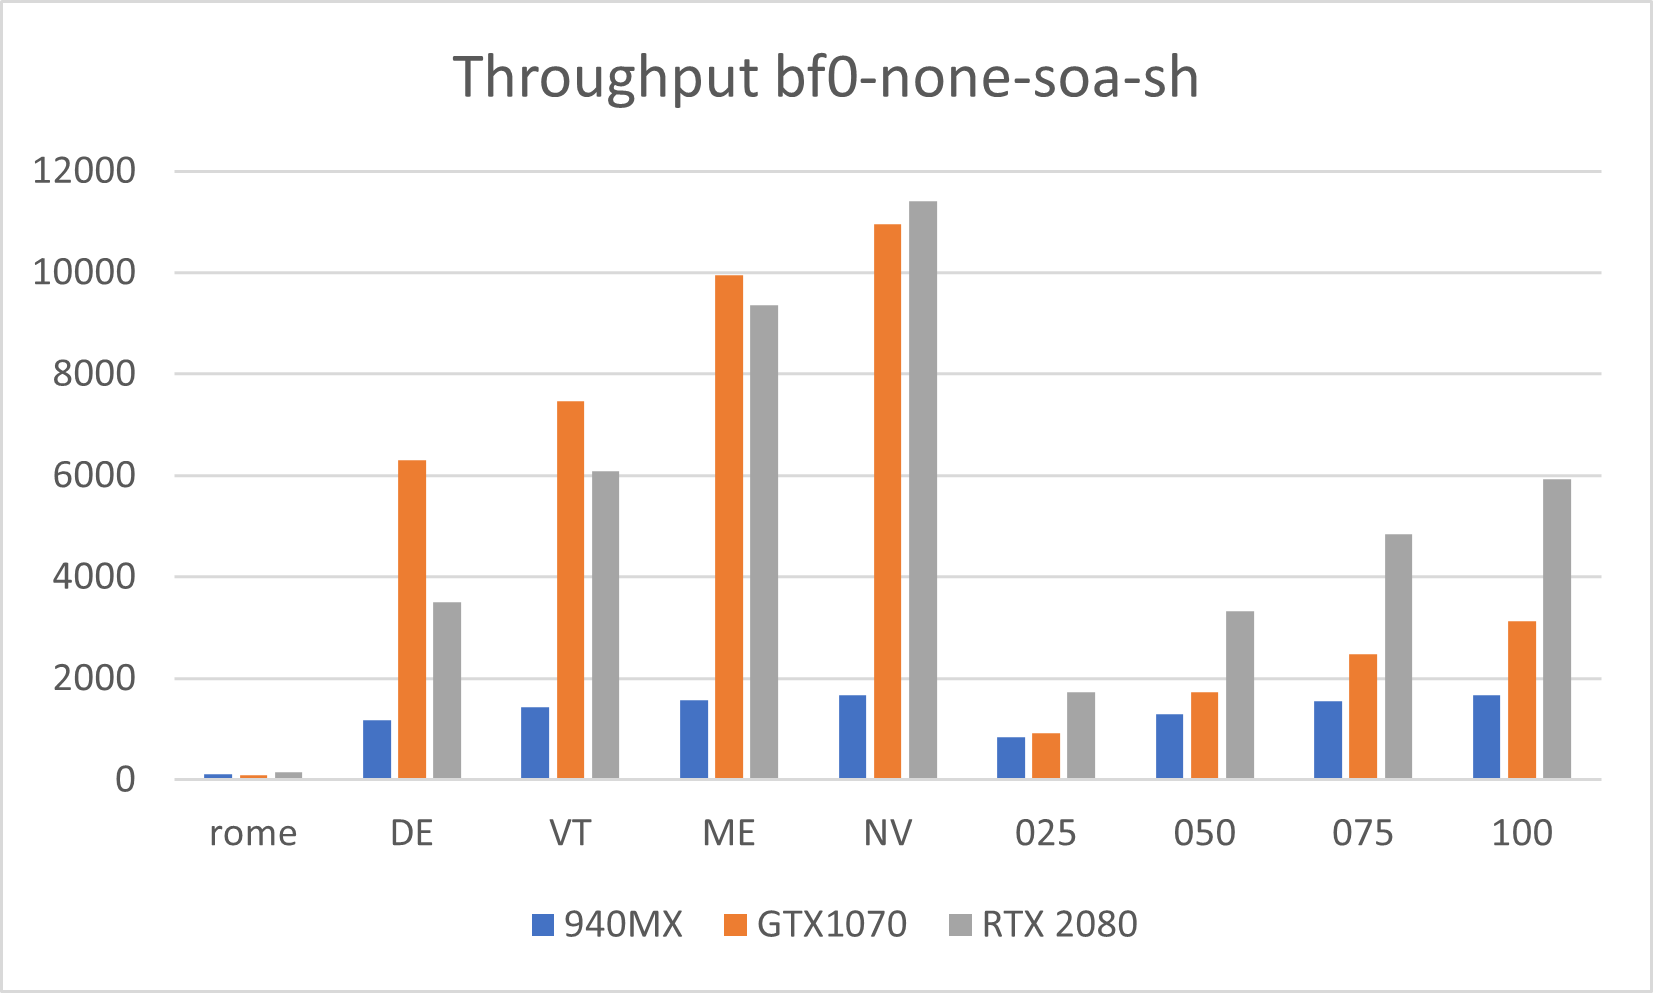
\includegraphics[width=\textwidth]{throughput_bf0-none-soa-sh}
		\end{subfigure}
		\caption{Throughput algoritmi \texttt{bf0-none}}
		\label{fig:throughput_bf0-none}
	\end{figure}
	
	\begin{figure}[b]
		\centering
		\begin{subfigure}{.5\textwidth}
			\centering
			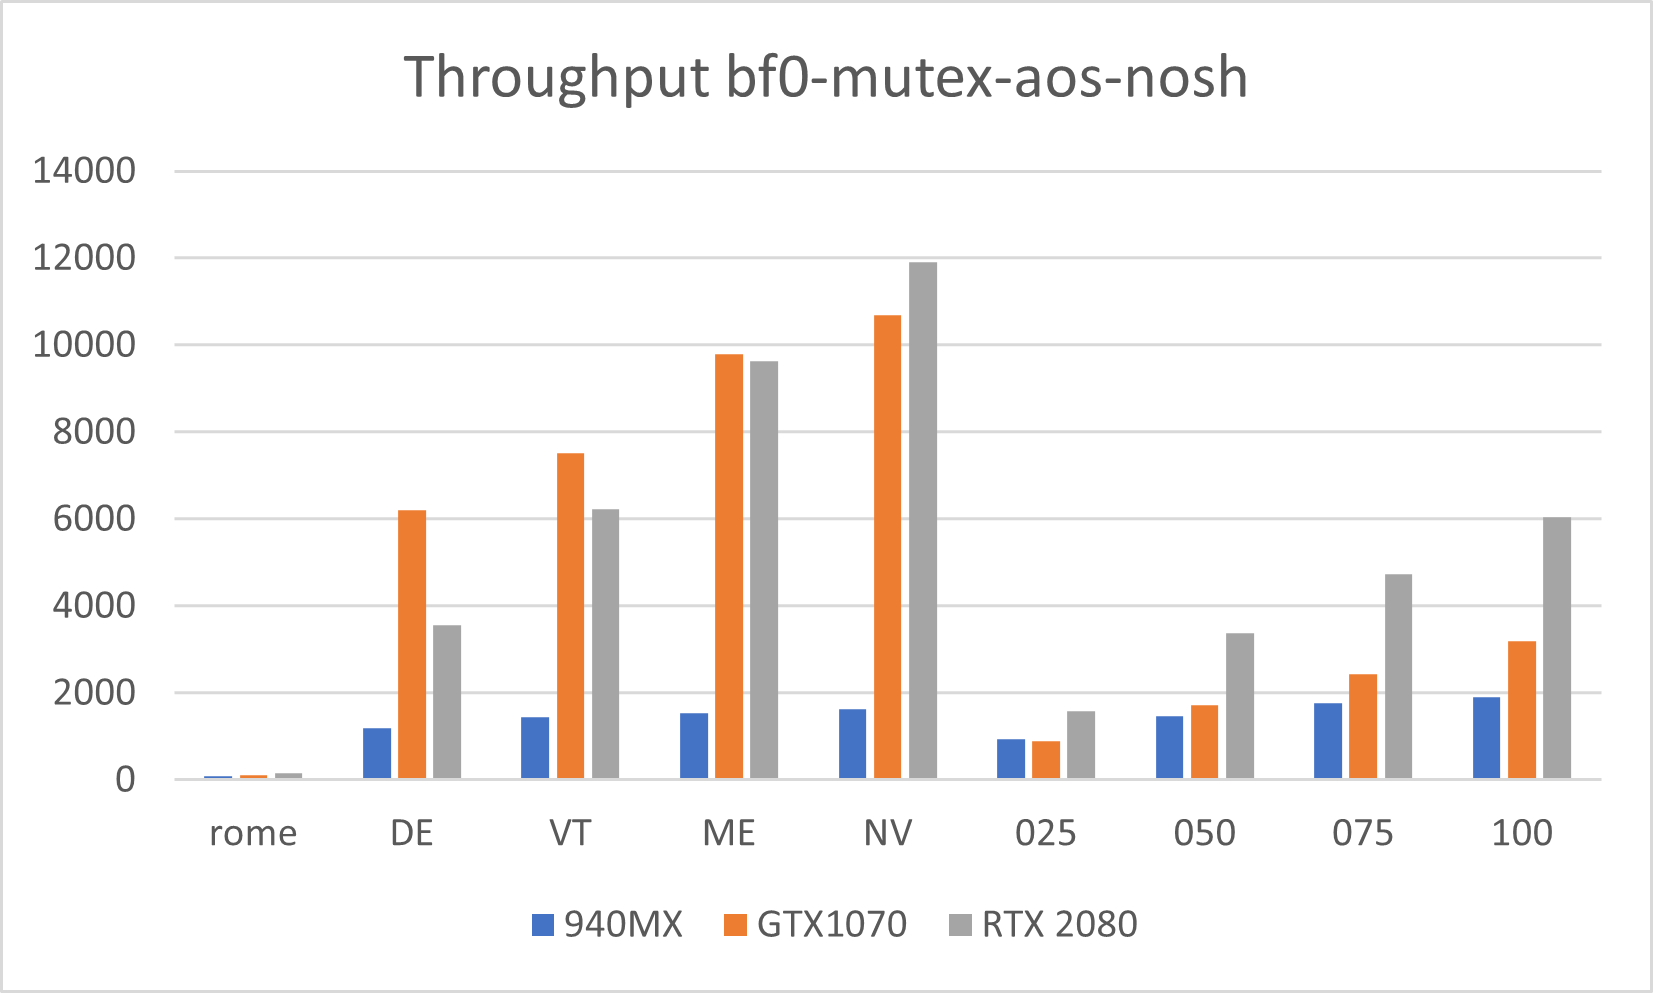
\includegraphics[width=\textwidth]{throughput_bf0-mutex-aos-nosh}
		\end{subfigure}%
		\begin{subfigure}{.5\textwidth}
			\centering
			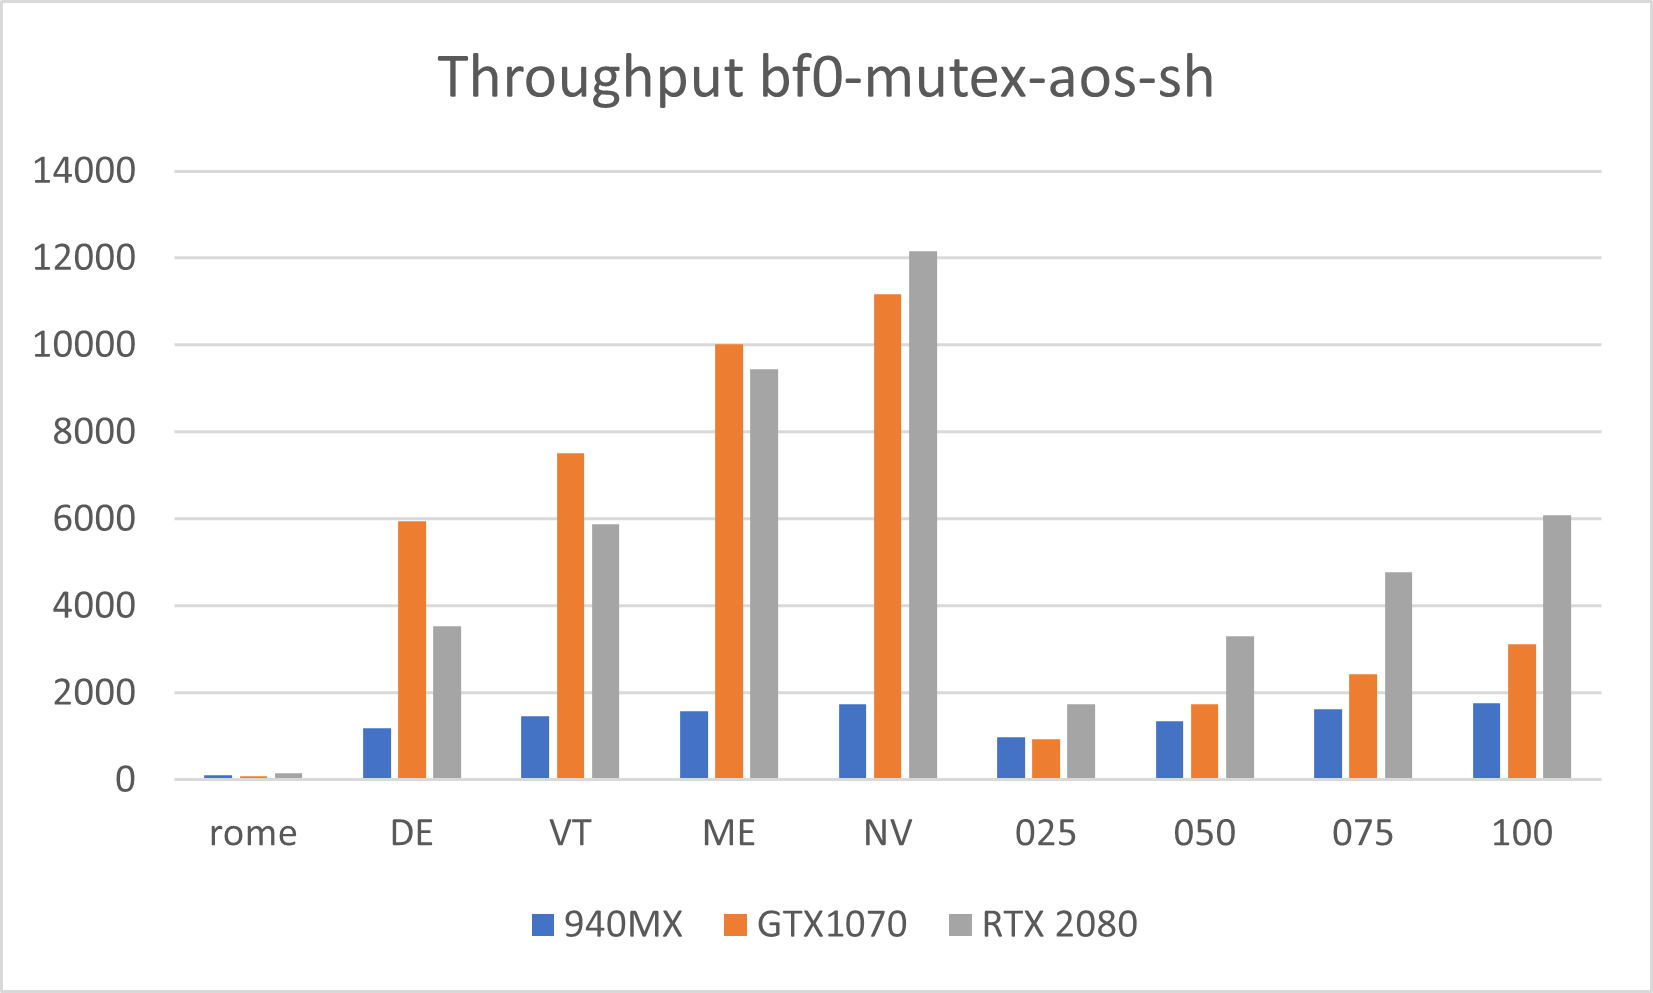
\includegraphics[width=\textwidth]{throughput_bf0-mutex-aos-sh}
		\end{subfigure}
		\begin{subfigure}{.5\textwidth}
			\centering
			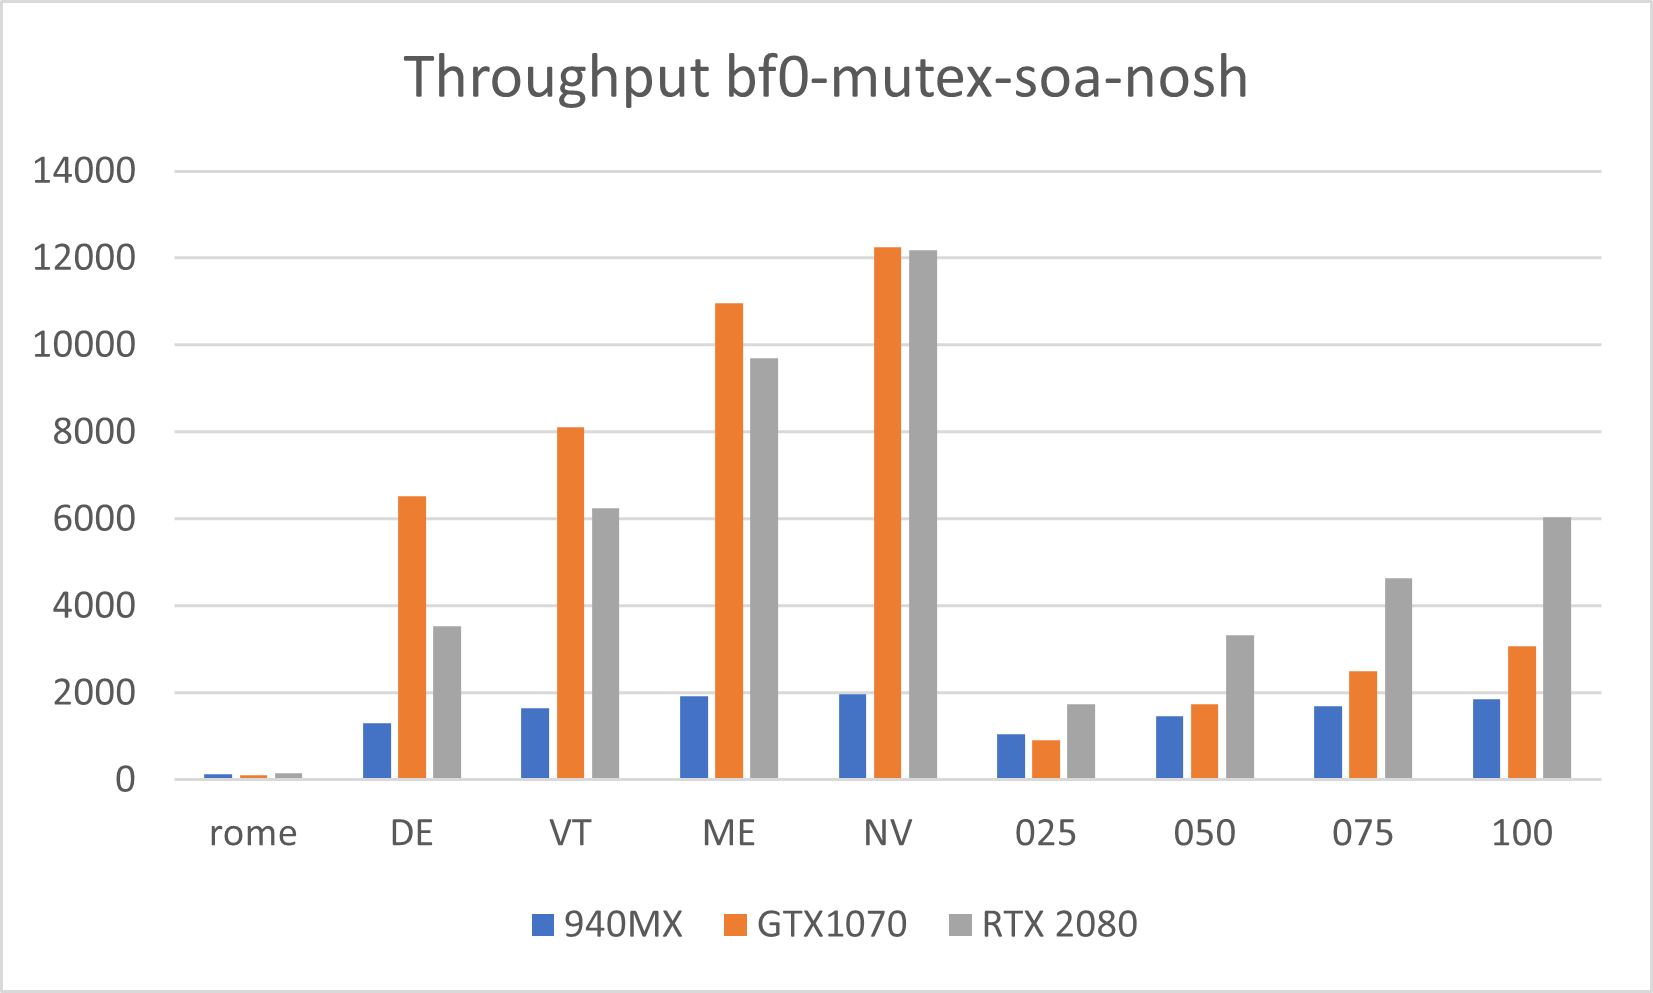
\includegraphics[width=\textwidth]{throughput_bf0-mutex-soa-nosh}
		\end{subfigure}%
		\begin{subfigure}{.5\textwidth}
			\centering
			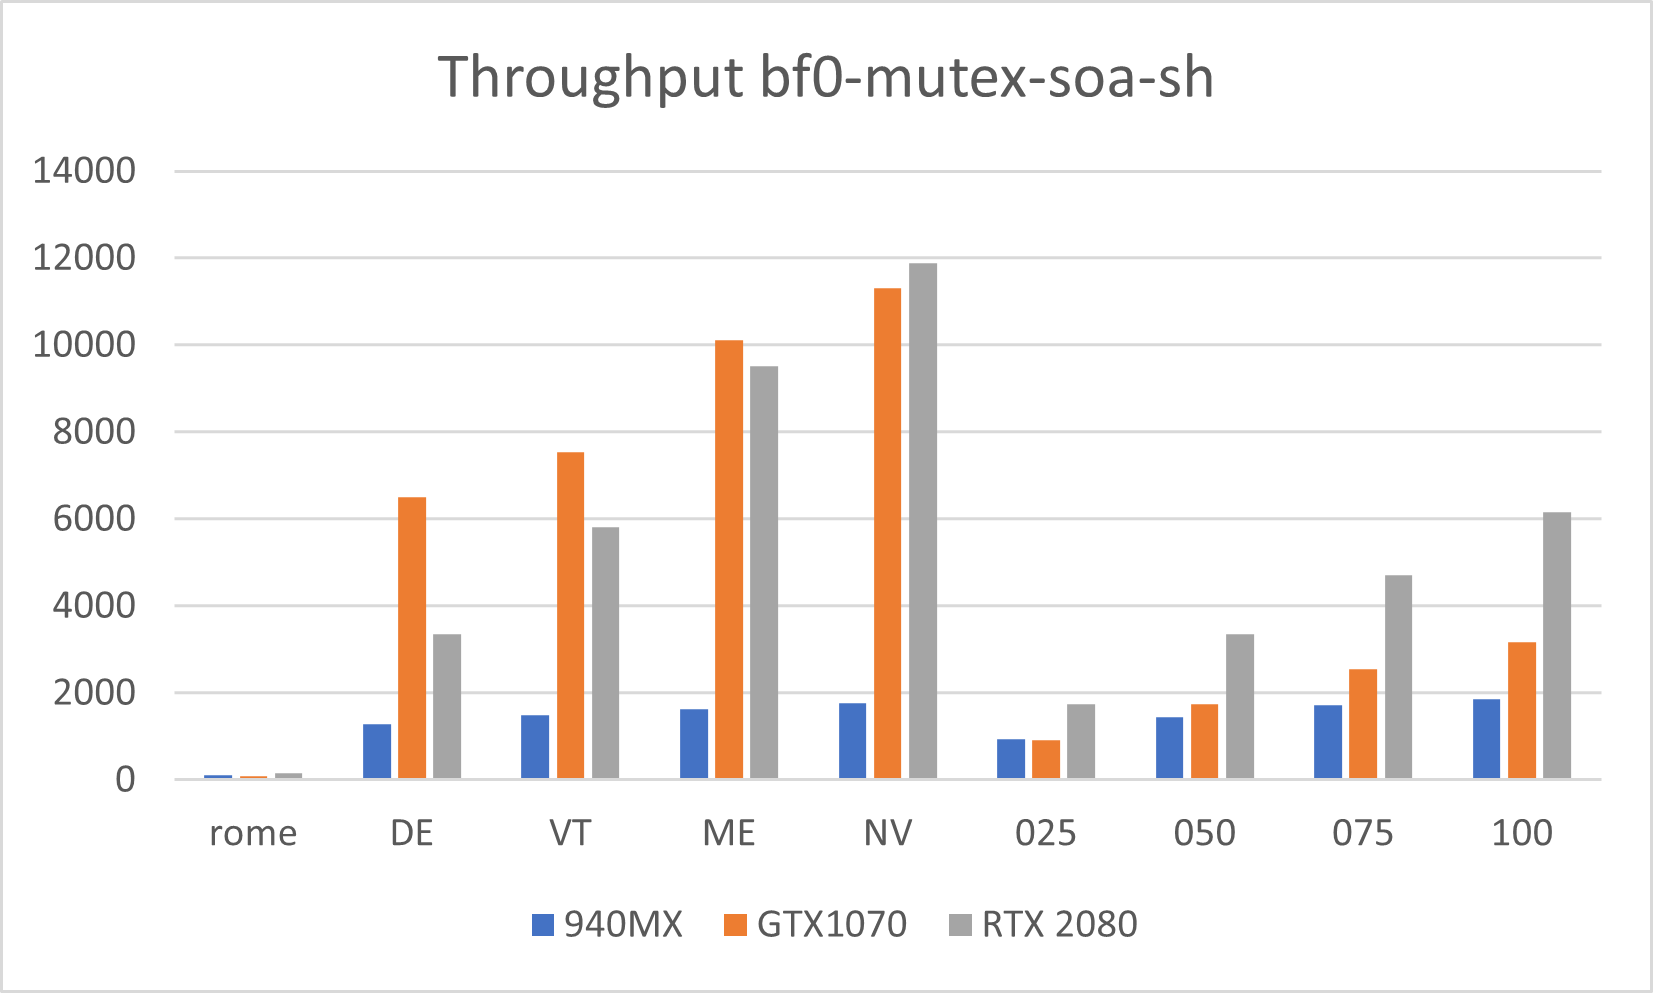
\includegraphics[width=\textwidth]{throughput_bf0-mutex-soa-sh}
		\end{subfigure}
		\caption{Throughput algoritmi \texttt{bf0-mutex}}
		\label{fig:throughput_bf0-mutex}
	\end{figure}

	In figura \ref{fig:throughput_bf1} osserviamo come l'impiego di un singolo blocco per l'esecuzione dei kernel, delle versioni \texttt{bf1}, abbia determinato una riduzione di prestazioni pari a circa un ordine di grandezza, nel caso migliore, rispetto agli algoritmi \texttt{bf0}.
	
	I valori misurati sui grafi \texttt{rome} e \texttt{DE} sono prossimi a $0$ a causa dell'elevato tempo di esecuzione impiegato.

	\begin{figure}[b]
		\centering
		\begin{subfigure}{.5\textwidth}
			\centering
			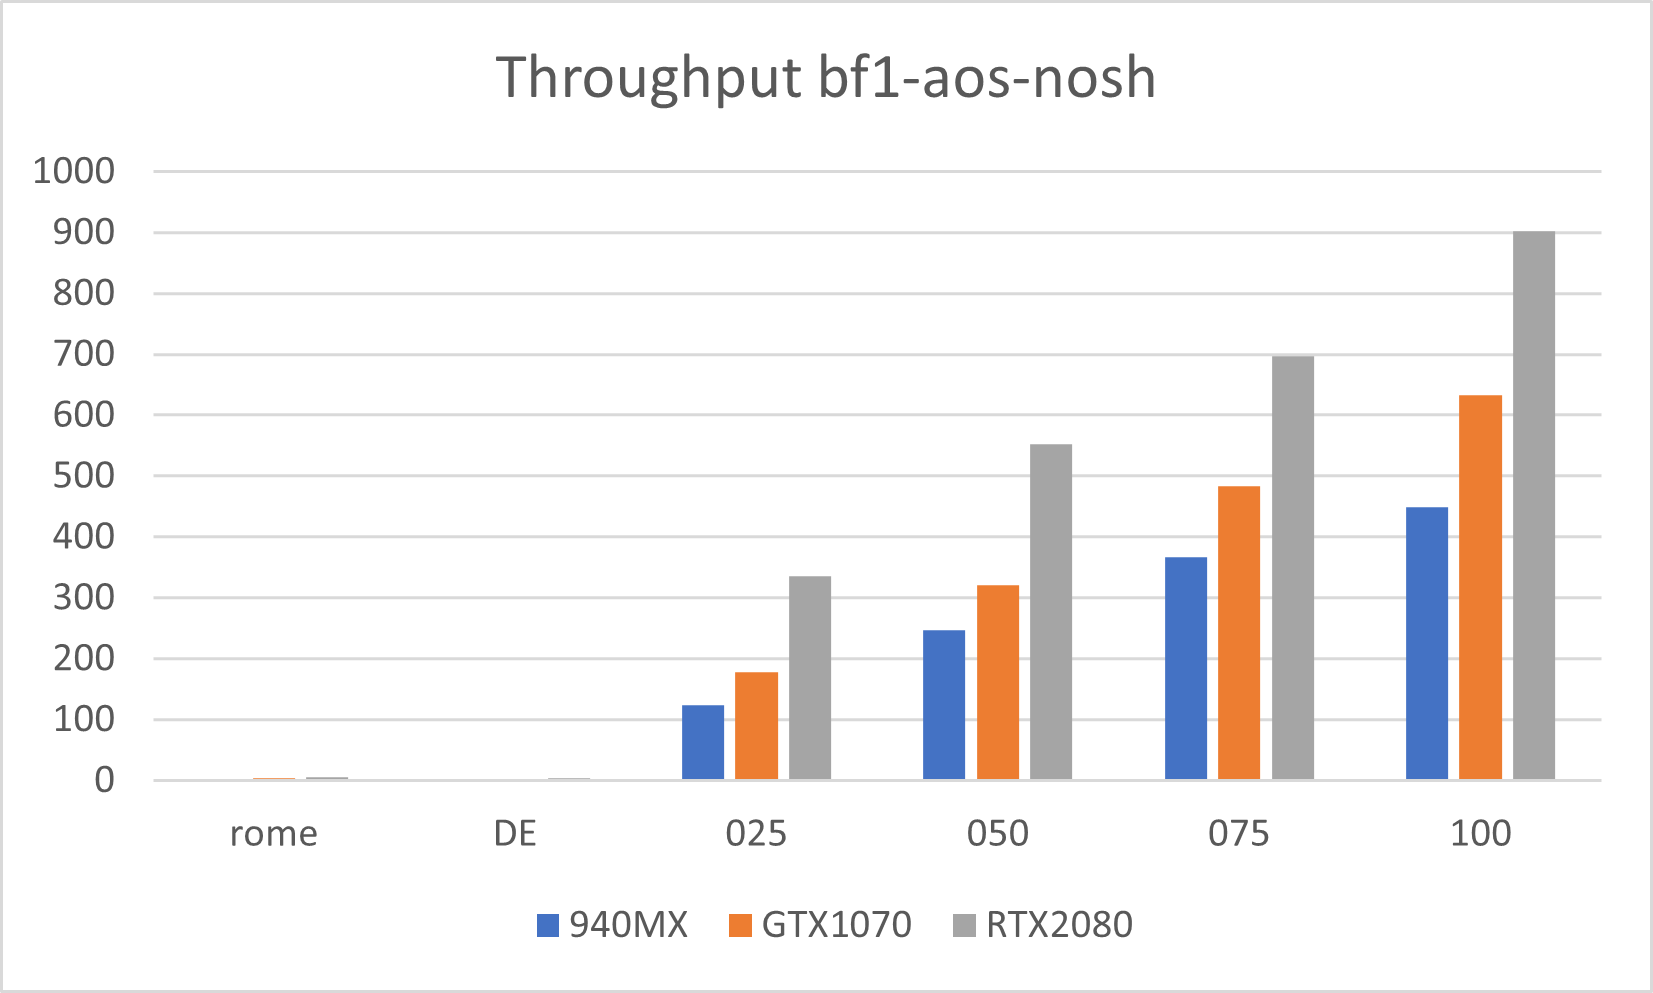
\includegraphics[width=\textwidth]{throughput_bf1-aos-nosh}
		\end{subfigure}%
		\begin{subfigure}{.5\textwidth}
			\centering
			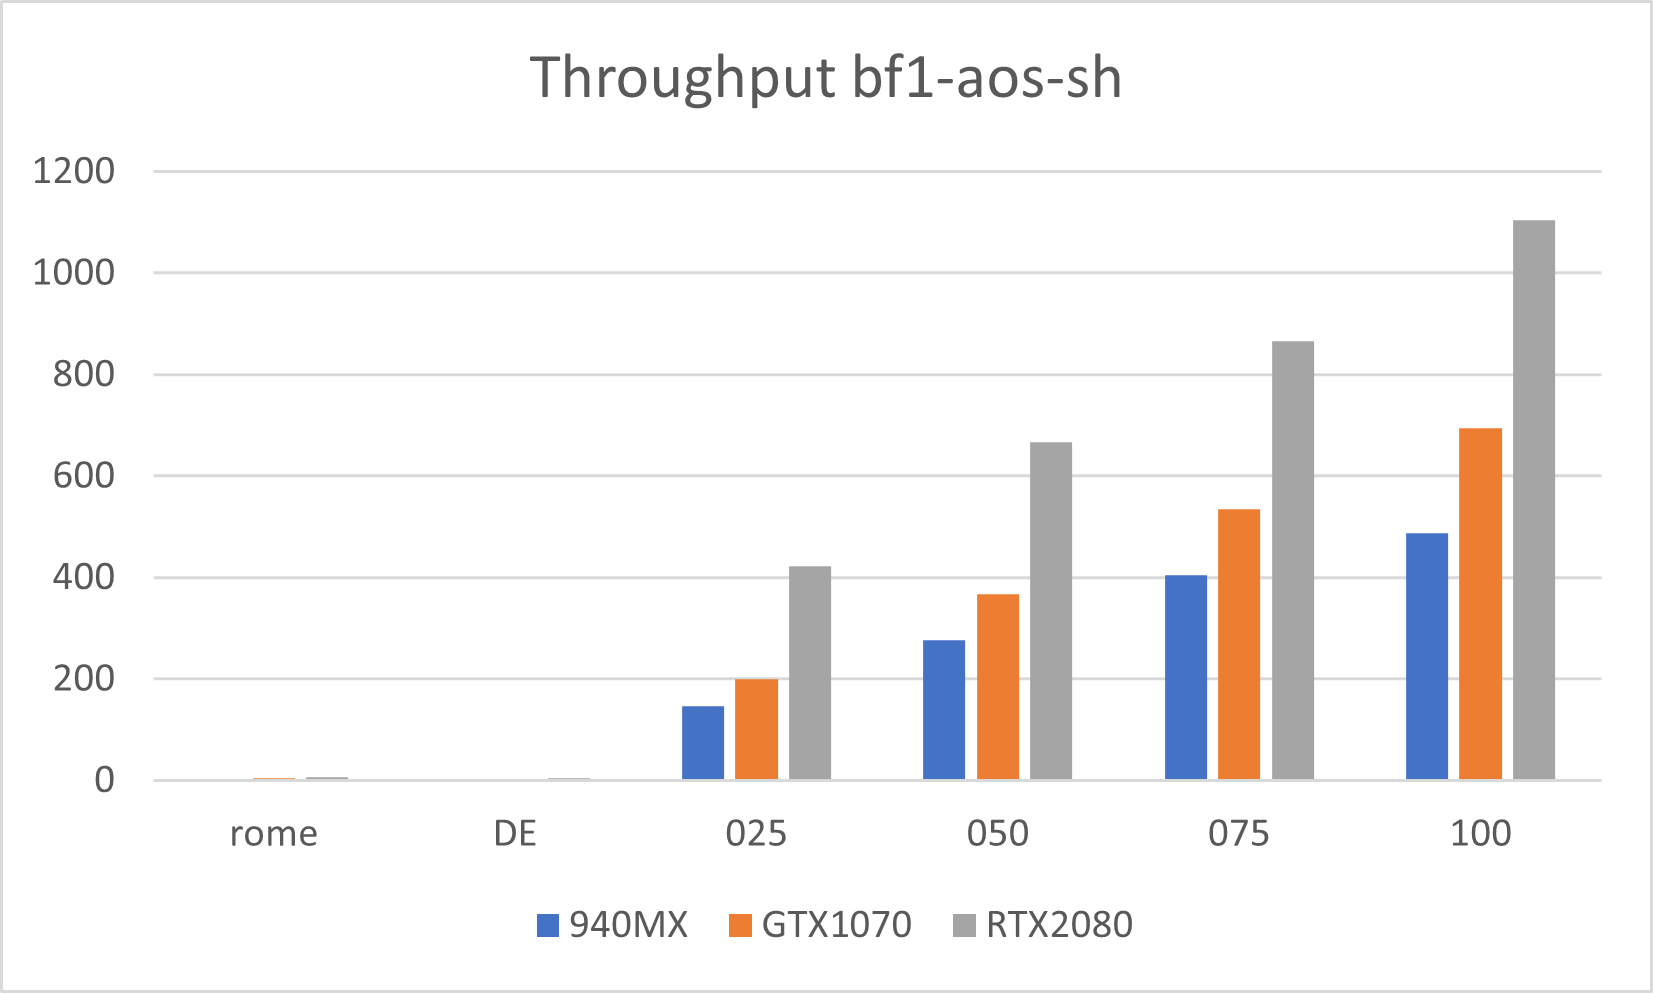
\includegraphics[width=\textwidth]{throughput_bf1-aos-sh}
		\end{subfigure}
		\begin{subfigure}{.5\textwidth}
			\centering
			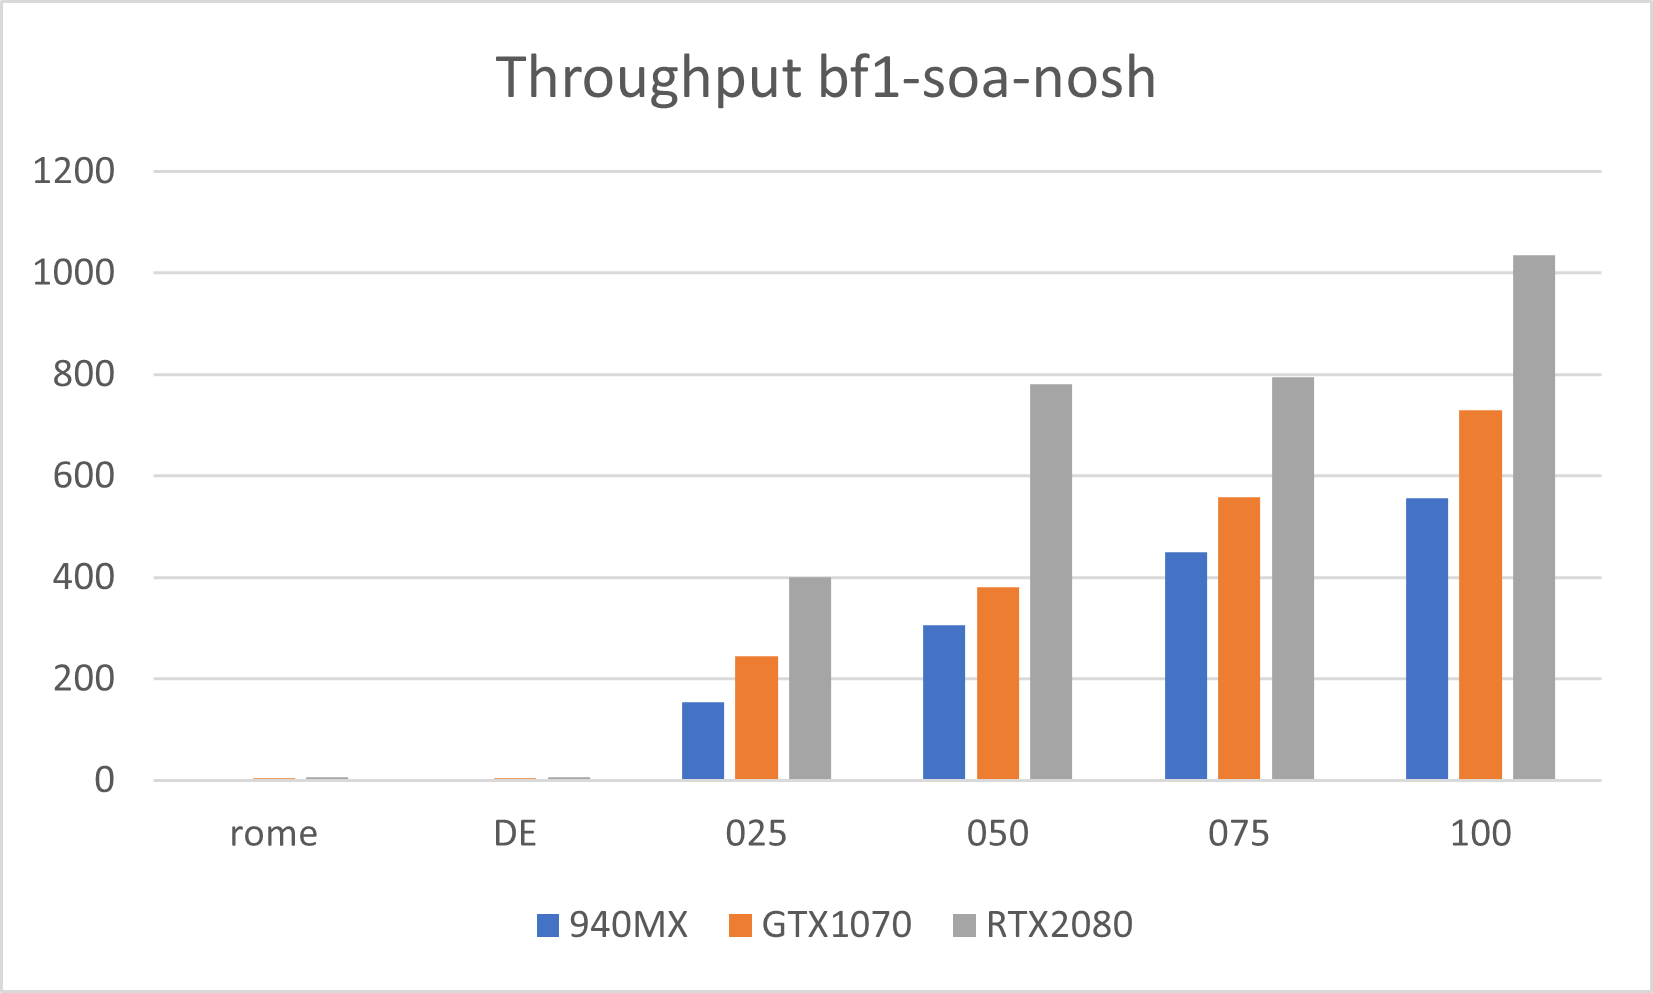
\includegraphics[width=\textwidth]{throughput_bf1-soa-nosh}
		\end{subfigure}%
		\begin{subfigure}{.5\textwidth}
			\centering
			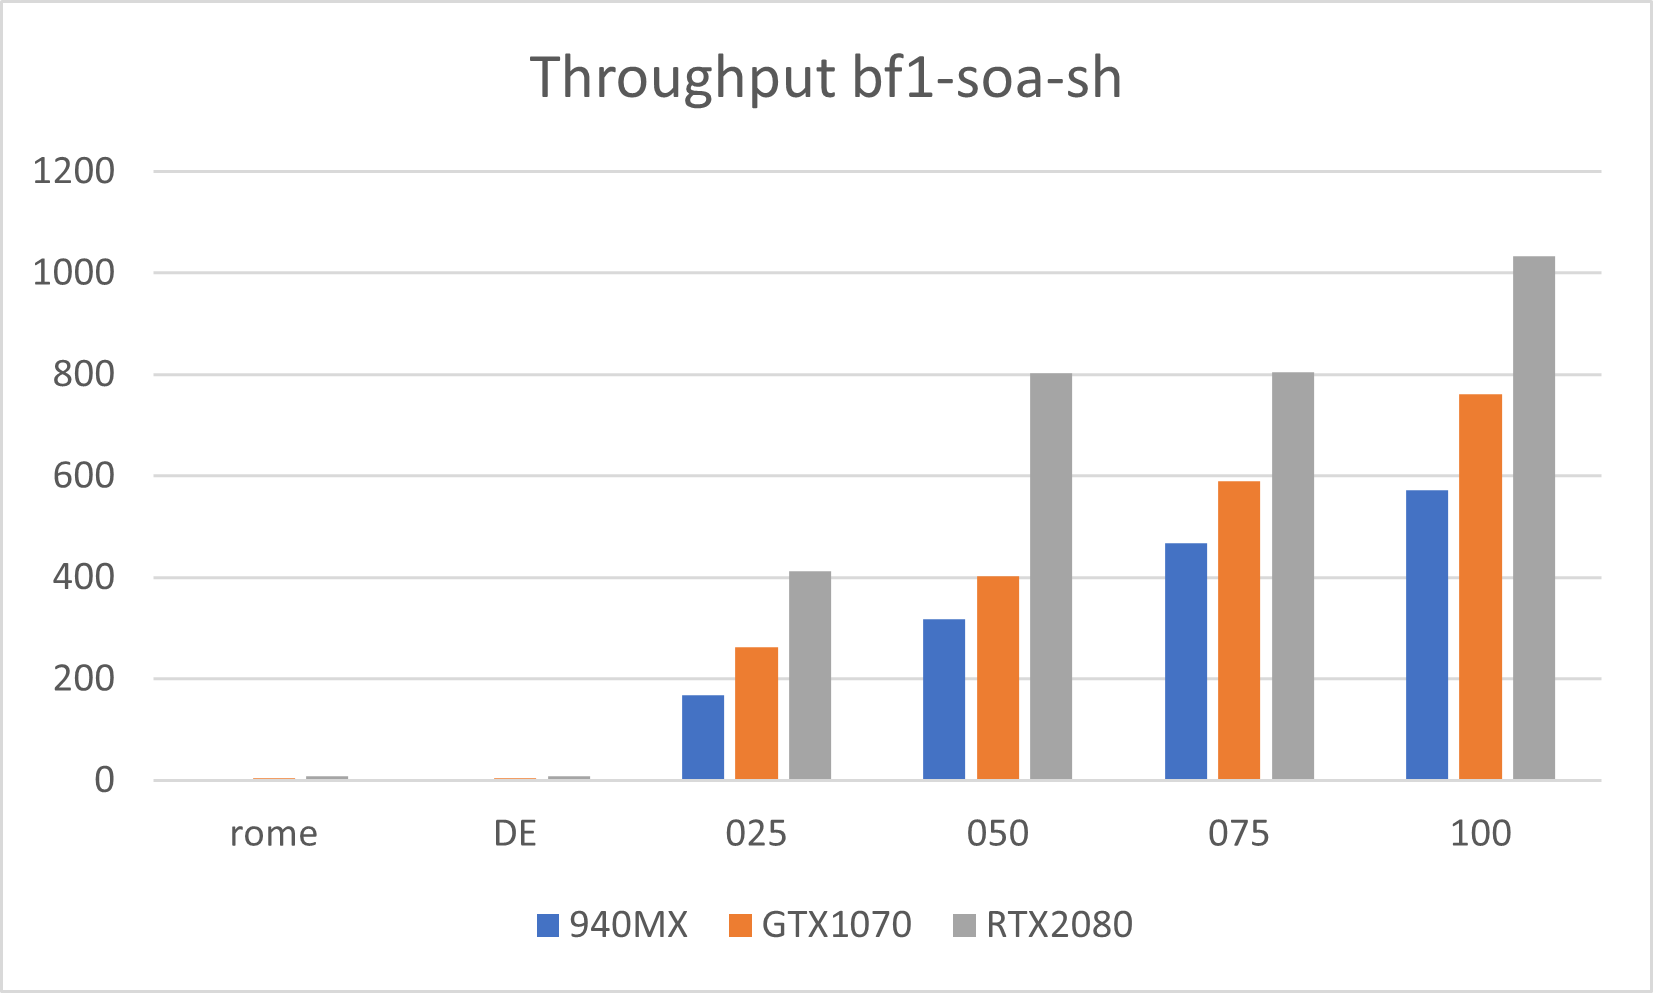
\includegraphics[width=\textwidth]{throughput_bf1-soa-sh}
		\end{subfigure}
		\caption{Throughput algoritmi \texttt{bf1}}
		\label{fig:throughput_bf1}
	\end{figure}

	Come già osservato per lo speedup, in figura \ref{fig:throughput_bf2} osserviamo un aumento delle prestazioni, rispetto agli algoritmi \texttt{bf1}, di almeno ad un fattore 4. Nonostante sia un incremento importante, il throughput delle versioni \texttt{bf2} risulta di molto inferiore rispetto alle prestazioni degli algoritmi \texttt{bf0}.

	\begin{figure}[b]
		\centering
		\begin{subfigure}{.5\textwidth}
			\centering
			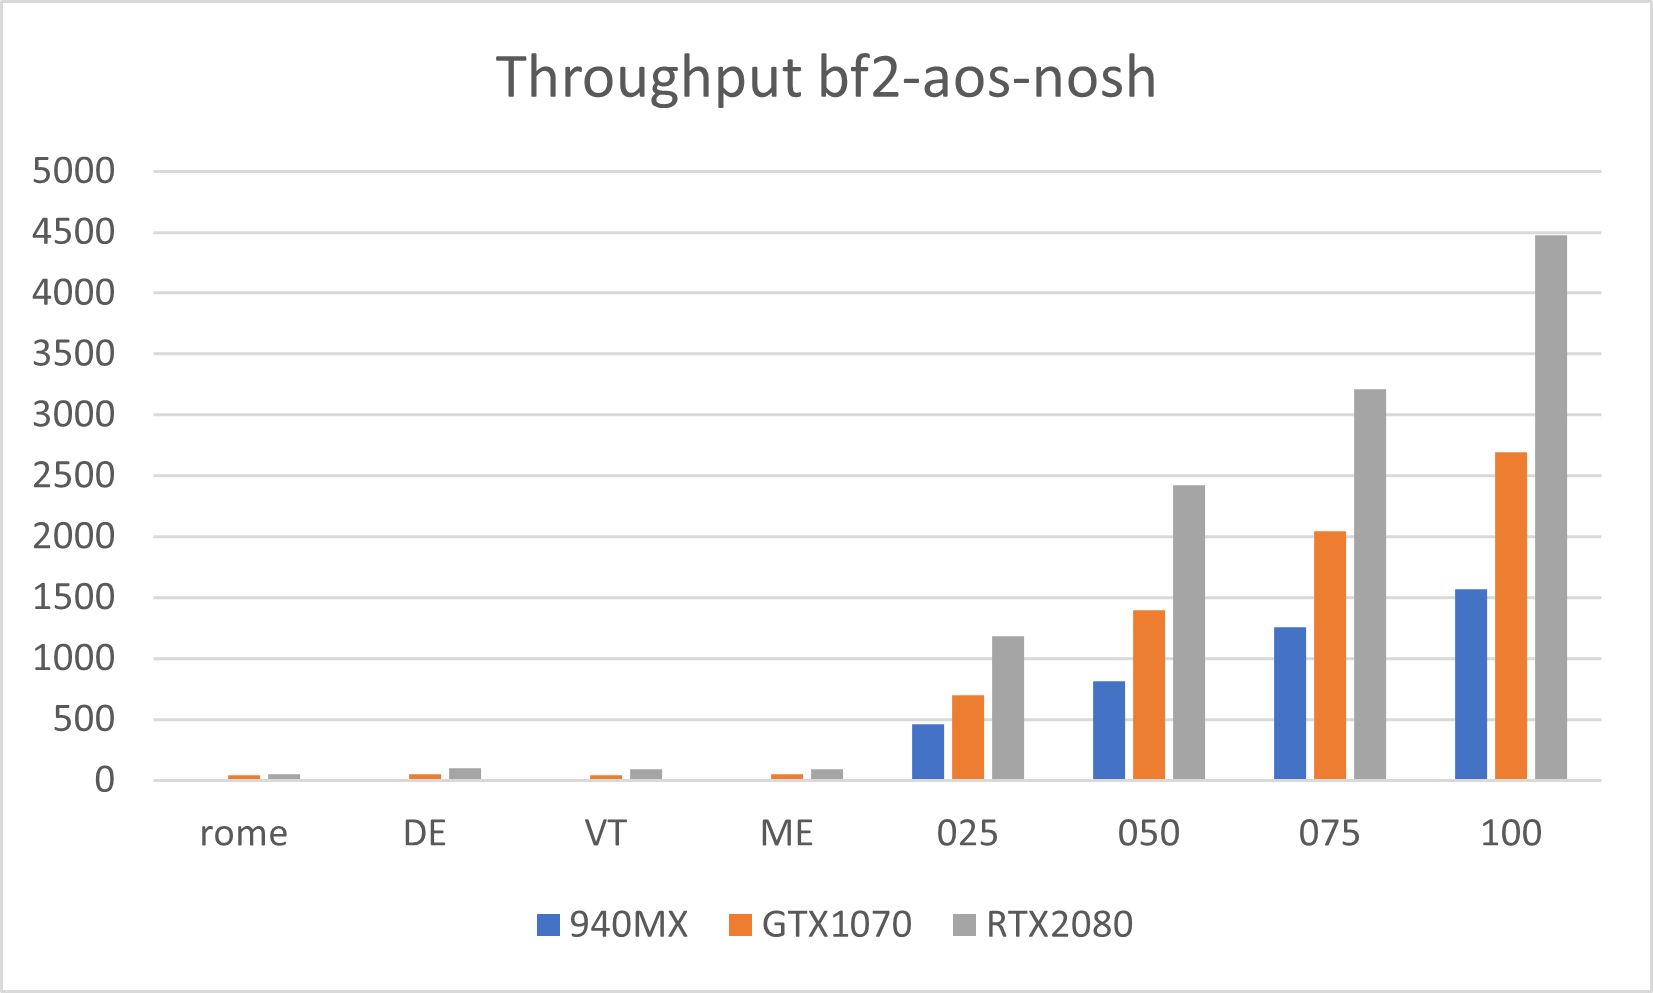
\includegraphics[width=\textwidth]{throughput_bf2-aos-nosh}
		\end{subfigure}%
		\begin{subfigure}{.5\textwidth}
			\centering
			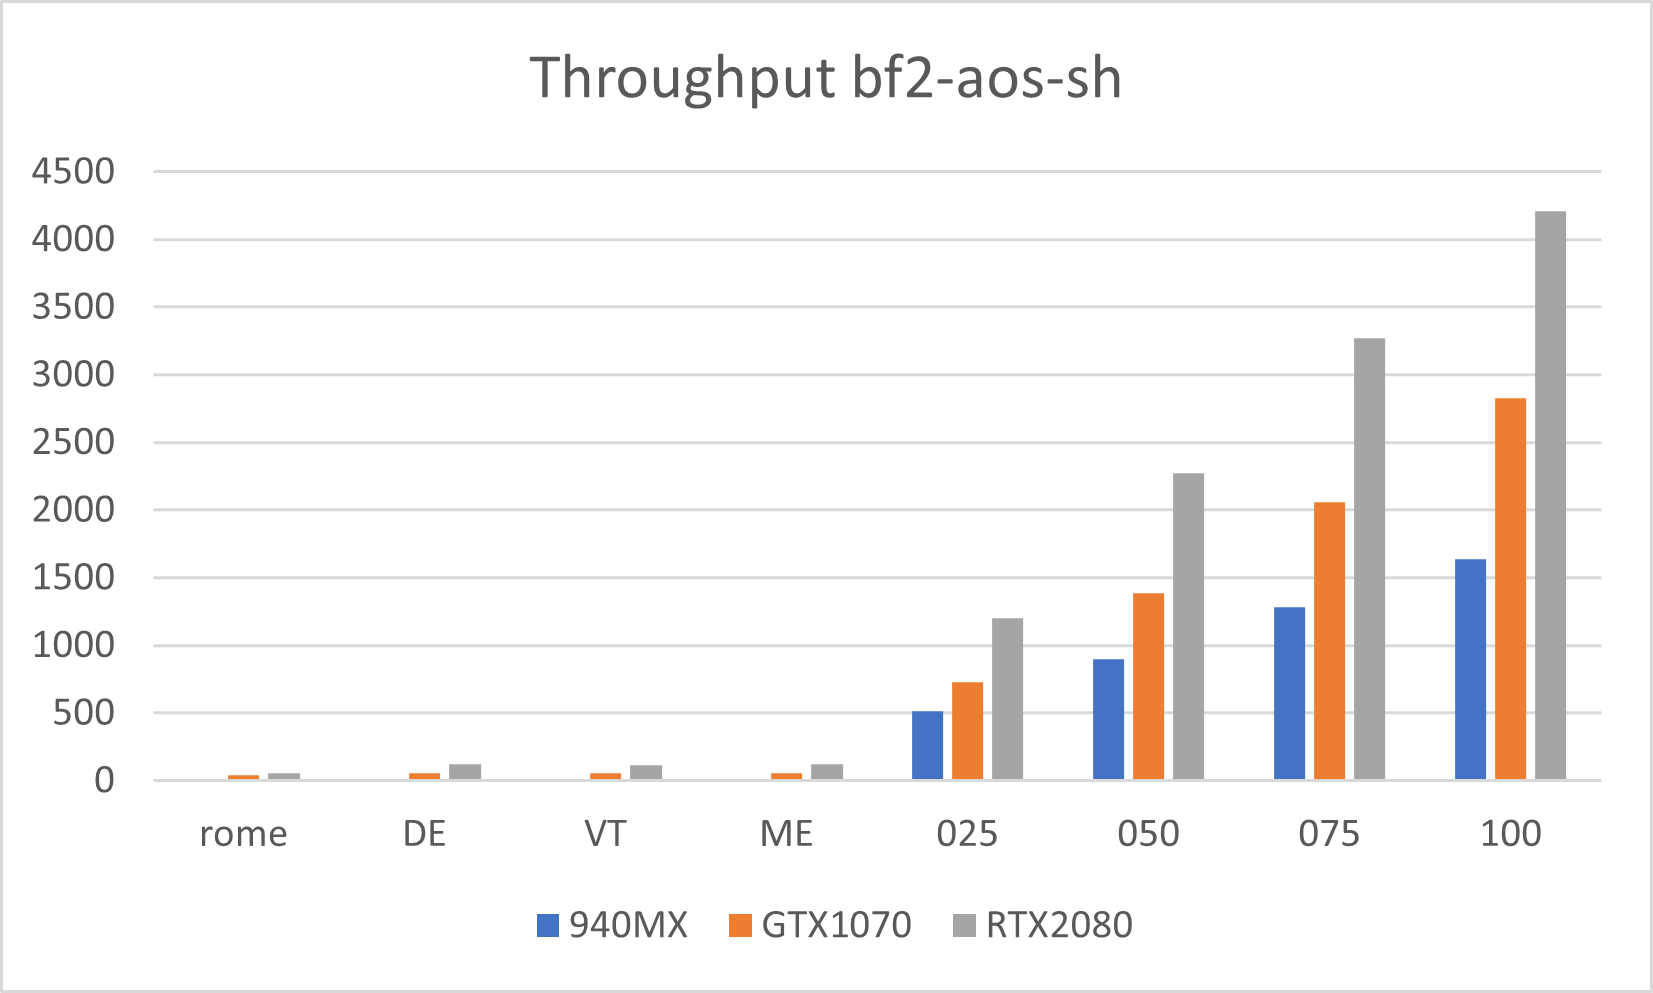
\includegraphics[width=\textwidth]{throughput_bf2-aos-sh}
		\end{subfigure}
		\begin{subfigure}{.5\textwidth}
			\centering
			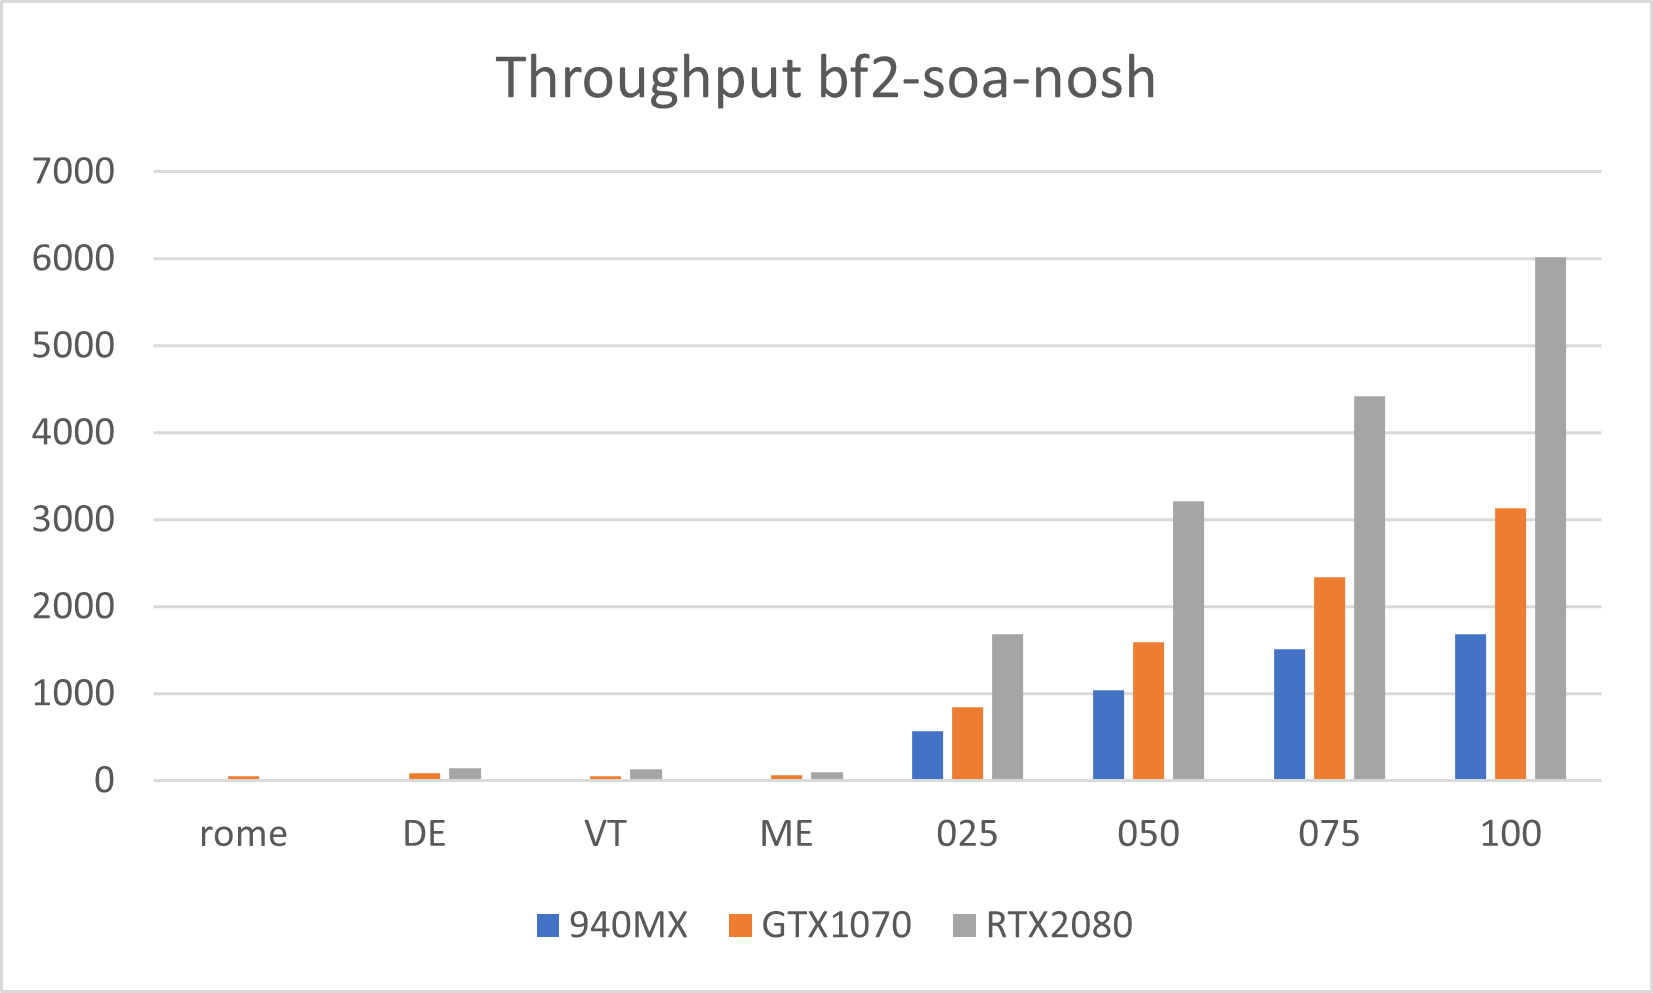
\includegraphics[width=\textwidth]{throughput_bf2-soa-nosh}
		\end{subfigure}%
		\caption{Throughput algoritmi \texttt{bf2}}
		\label{fig:throughput_bf2}
	\end{figure}
	
	\chapter*{Conclusioni e sviluppi futuri}
	In questa tesi sono state analizzate varie implementazioni dell'algoritmo di Bellman-Ford in CUDA, con un'ampia esplorazione delle ottimizzazioni possibili e molti test effettuati. Nonostante la differenza sia molto ridotta rispetto agli altri algoritmi della stessa famiglia, l'algoritmo effettivamente più veloce risulta essere \texttt{bf0-none-soa-nosh}, che riesce a processare in poco più di 13 secondi la mappa stradale del Nevada, uno stato grande quasi quanto l'Italia, sulla scheda RTX 2080. Se consideriamo che l'algoritmo implementato è assolutamente privo di ogni ottimizzazione, questo dato fa riflettere sulle potenzialità che Bellman-Ford presenta riguardo all'impiego su GPGPU. Per questo motivo, un possibile sviluppo futuro di questo progetto consisterebbe nell'implementazione delle varie ottimizzazioni proposte negli anni. Inoltre, la struttura di Bellman-Ford suggerisce una facile divisione del lavoro per un sistema multi-GPU. Effettuando anche questa ottimizzazione, l'algoritmo potrebbe essere anche utilizzato per processare il grafo contenente la struttura di Internet in tempi non proibitivi.
	
	\printbibliography
	
	\chapter*{Ringraziamenti}
	Voglio ringraziare la mia famiglia per il sostegno e il supporto che mi hanno dato. Un sentito ringraziamento va alla mia fidanzata e a tutti gli amici, dentro e fuori l'università, per avermi sempre dato la forza di migliorare e andare avanti. Un ringraziamento speciale va all'amico Lorenzo Di Ghionno per avermi concesso di utilizzare la sua RTX 2080 per la realizzazione di questa tesi. Ringrazio tutti i professori del corso di laurea che hanno contribuito alla mia formazione e aiutato ad arrivare fin qui. Ultimo ma non per ultimo, desidero ringraziare il professore Moreno Marzolla per avermi sempre aiutato con simpatia e professionalità.
	
\end{document}